\documentclass{article}
	\usepackage{beppe_package}
	\usepackage[a4paper, left=1.5cm, bottom=2.5cm, right=1.5cm]{geometry}
	
	\renewcommand{\a}{(a)}
	\renewcommand{\b}{(b)}
	\renewcommand{\c}{(c)}
	\renewcommand{\t}[1]{\textit{ #1}}
	\renewcommand{\vec}[1]{\mathbf{#1}}
	
	\title{Checklist di Fisica 3}
	\author{Giuseppe Bogna, Edoardo Centamori}
	\date{Anno accademico 2017-2018}

\begin{document}
	\maketitle
	
	\begin{abstract}
		Questo pdf contiene le domande e le risposte per l'esame di Fisica 3. I livelli di difficoltà sono\begin{itemize}
			\item domande \a : richiedono una risposta pronta e sicura;
			\item domande \b : sono domande o esercizi la cui risposta può non essere immediata;
			\item domande \c : sono argomenti facoltativi.
		\end{itemize}
		Per ovvi motivi, le domande a scelta non sono state tutte risolte. Inoltre, buona parte delle stime numeriche sono assenti.f
	\end{abstract}

\tableofcontents

	\section{Prerequisiti}
	\begin{enumerate}
		\item \a \t{Dare la definizione di 4-vettore covariante e controvariante.}
		Un quadrivettore controvariante $x^\mu$ è una quaterna $(x^0,x^1,x^2,x^3)$ che sotto trasformazioni di Lorentz trasforma nel seguente modo
		\[x'^{\mu}=\tensor{\Lambda}{^\mu_\nu}x^\nu\]
		dove $\tensor{\Lambda}{^\mu_\nu}$ è una qualche matrice del gruppo di Lorentz. La forma più generale di tale matrice è
		\[\tensor{\Lambda}{^\mu_\nu}=\left(\begin{array}{c | c c c}
		1&0&0&0\\\hline0&&&\\0&&\mathcal{R}&\\0&&&
		\end{array}\right)\left(\begin{array}{c c c c}
		\gamma&-\gamma\beta&0&0\\-\gamma\beta&\gamma&0&0\\0&0&1&0\\0&0&0&1
		\end{array}\right)\left(\begin{array}{c | c c c}
		1&0&0&0\\\hline0&&&\\0&&\mathcal{R}'&\\0&&&
		\end{array}\right)\]
		con $\mathcal{R},\mathcal{R}'\in\mathrm{O}_3$. Se consideriamo ancora la trasformazione data da $\tensor{\Lambda}{^\mu_\nu}$, un quadrivettore covariante $x_\mu$ è sempre una quaterna $(x_0,x_1,x_2,x_3)$, che trasforma invece come
		\[x'_\mu=\tensor{\Lambda}{_\mu^\nu}x_\nu\]
		dove $\tensor{\Lambda}{_\mu^\nu}$ è
		\[\tensor{\Lambda}{_\mu^\nu}=g_{\mu\alpha}\tensor{\Lambda}{^\alpha_\beta}g^{\beta\nu}\]
		avendo posto $g_{\mu\nu}=g^{\mu\nu}=\textrm{diag}(1,-1,-1,-1)$.
		\item \a\t{Definire le quantità $\beta$ e $\gamma$ per le trasformazioni di Lorentz.} Presi due sistemi di riferimento inerziali con origini $O$ e $O'$, $\beta$ è la velocità (in unità $c$) di $O'$ rispetto ad $O$, mentre
		\[\gamma=\frac{1}{\sqrt{1-\beta^2}}\]
		\item\a\t{Definire il prodotto scalare di due 4-vettori.} Presi $x^\mu=(x^0,\vec{x})$ e $y^\mu=(y^0,\vec{y})$, si definisce il loro prodotto $x^\mu y_\nu$ come
		\[x^\mu y_\mu=x^0y^0-\vec{x}\cdot\vec{y}\]
		Dato che $y_\mu=g_{\mu\nu}y^\nu$, e dato che il tensore metrico è preservato dai boost lungo gli assi e dalle rotazioni, il prodotto di due 4-vettori è un invariante di Lorentz.
		\item\a\t{Definire il modulo di un 4-vettore.} Se $x^\mu$ è un quadrivettore, il suo modulo è dato da
		\[|x|^2=x^\mu x_\mu\]
		Dato che il tensore metrico non è definito positivo, il modulo quadro di un quadrivettore può essere positivo, negativo o nullo.
		\item\a\t{Scrivere le trasformazioni di Lorentz per il boost lungo un asse (asse x).} Per un boost lungo l'asse $x$ si ha
		\[\begin{cases}
		ct'=\gamma(ct-\beta x)\\x'=\gamma(x-\beta ct)\\y'=y\\z'=z
		\end{cases}\]
		o, in forma matriciale
		\[\left(\begin{array}{c}
		ct'\\x'\\y'\\z'
		\end{array}\right)=\left(\begin{array}{c c c c}
		\gamma&-\gamma\beta&0&0\\-\gamma\beta&\gamma&0&0\\0&0&1&0\\0&0&0&1
		\end{array}\right)\left(\begin{array}{c}
		ct\\x\\y\\z
		\end{array}\right)\]
		\item\a\t{Definire le derivate in 4-dimensioni, la quadridivergenza, il differenziale di uno scalare di Lorentz, l'operatore di D'Alembert.} Definiamo gli operatori $\partial^\mu$ e $\partial_\mu$ come
		\begin{align*}
			\partial^\mu&=\left(\frac{1}{c}\pder{}{t},-\nabla\right)\\
			\partial_\mu&=\left(\frac{1}{c}\pder{}{t},\nabla\right)
		\end{align*}
		Preso un generico campo tensoriale, la sua quadridivergenza (rispetto a un qualche indice) è la contrazione tra l'operatore $\partial^\mu$ e l'indice stesso (se quest'ultimo è covariante), tra l'operatore $\partial_\mu$ e l'indice stesso (se quest'ultimo è controvariante). Ad esempio, se $v^\mu=(v^0,\vec{v})$ è un campo vettoriale la sua quadridivergenza è
		\[\partial_\mu v^\mu=\frac{1}{c}\pder{v^0}{t}+\nabla\cdot \vec{v}\]
		Se invece $\phi$ è un invariante di Lorentz, il suo differenziale è
		\[\d\phi=\d x^\mu\partial_\mu\phi=\pder{\phi}{t}\d t+(\d \vec{x}\cdot\nabla)\phi\]
		Infine, l'operatore di D'Alembert è
		\[\square=\partial_\mu\partial^\mu=\frac{1}{c^2}\pder[2]{}{t}-\lap\]
		\item\a\t{Definire il tempo proprio e dare la relazione (differenziale) fra tempo proprio e tempo nel sistema in cui si osserva il moto.}
		Si sa che l'intervallo $\d s^2=|\d x^\mu|^2$ è uno scalare di Lorentz. Nel sistema tangente si ha chiaramente $\d x^\mu=(c\d\tau,0)$, dove $\d\tau$ è il tempo proprio (infinitesimo). Di conseguenza, si ottiene
		\[c^2\d\tau^2=c^2\d t^2-|\d \vec{x}|^2=c^2\d t^2-|\vec{v}|^2\d t^2\]
		e infine
		\[\d \tau=\d t/\gamma\]
		\item\a\t{Dare la definizione di invariante di Lorentz.} Un invariante di Lorentz è una grandezza che viene lasciata invariata dalle trasformazioni di Lorentz, ossia è uguale in tutti i sistemi di riferimento inerziali.
		\item\a\t{Definire la 4-velocità e il 4-impulso di un punto materiale di massa $m$, esprimere le loro unità di misura nei sistemi MKS e $\hbar=c=1$, dimostrare che il loro modulo è costante.} La 4-velocità e il 4-impulso sono rispettivamente
		\begin{align*}
			u^\mu&=\der{x^\mu}{\tau}=(\gamma c,\gamma\vec{v})\\p^\mu&=m u^\mu
		\end{align*}
		In MKS $u^\mu$ si misura in m/s e $p^\mu$ in kg$\cdot$ m/s, mentre in unità $\hbar=c=1$ $u^\mu$ è adimensionale e $p^\mu$ si misura in kg. I loro moduli sono rispettivamente
		\begin{align*}
			u^\mu u_\mu&=\gamma^2c^2-\gamma^2v^2=c^2\\
			p^\mu p_\mu&=m^2u^\mu u_\mu=m^2c^2
		\end{align*}
		e dunque sono costanti.
		\item\a\t{Enunciare la legge di conservazione del 4-impulso.} Per un sistema isolato, cioè non sottoposto a forze esterne, il 4-impulso totale si conserva nel tempo.
		\item\a\t{Definire un tensore covariante di rango 2 e la sua traccia.} \`E il prodotto tensore di due quadrivettori covarianti. Di conseguenza, un tensore covariante $F_{\mu\nu}$ trasforma sotto trasformazioni di Lorentz come
		\[F'_{\mu\nu}=\tensor{\Lambda}{_\mu^\alpha}\tensor{\Lambda}{_\nu^\beta}F_{\alpha\beta}\]
		La traccia di $F$ è
		\[\tensor{F}{^\mu_\mu}=g^{\mu\nu}F_{\nu\mu}\]
		\item\a\t{Definire il tensore metrico $g_{\mu\nu}$.} $g_{\mu\nu}=\mathrm{diag}(1,-1,-1,-1)$.
		\item\a\t{Dare la definizione di tensore antisimmetrico di rango 2 ed indicare quali dei suoi elementi siano le componenti di un vettore polare e quali quelle di un vettore assiale.}
		Un tensore $F^{\mu\nu}$ di rango 2 è antisimmetrico se cambia segno sotto scambio degli indici, ossia se
		\[F^{\mu\nu}=-F^{\nu\mu}\]
		Se le componenti di $F^{\mu\nu}$ sono
		\[F^{\mu\nu}=\left(\begin{array}{c | c c c}
		0&v_x&v_y&v_z\\\hline
		-v_x&0&-w_z&w_y\\-v_y&w_z&0&-w_x\\-v_z&-w_y&w_x&0
		\end{array}\right)\]
		allora $\vec{v}=(v_x,v_y,v_z)$ è un vettore polare e $\vec{w}=(w_x,w_y,w_z)$ è un vettore assiale.
		\item\a\t{Definire quando una certa legge fisica è scritta in forma "relativisticamente covariante".} Una legge fisica è scritta in forma covariante se è un'uguaglianza tra due oggetti che trasformano allo stesso modo sotto cambi di sistema di riferimento, ossia se hanno gli stessi indici covarianti e controvarianti.
		\item\a\t{Enunciare o ricavare la legge relativistica di composizione delle velocità.} Supponiamo di avere un corpo puntiforme e siano $\vec{v},\vec{v}'$ le sue velocità rispetto a due sistemi inerziali $O,O'$. Se $\vec{w}=w\hat{x}$ è la velocità di $O'$ rispetto ad $O$. Allora si ha
		\begin{align*}
			v'_x&=\frac{v_x-w}{1-v_xw/c^2}\\v'_y&=\frac{v_y}{\gamma(1-v_xw/c^2)}\\v'_z&=\frac{v_z}{\gamma(1-v_xw/c^2)}
		\end{align*}
		dove $\gamma=(1-w^2/c^2)^{-1/2}$.
		\item\a\t{Dimostrare che il modulo di un 4-vettore ed il prodotto di due 4-vettori sono invarianti di Lorentz.} \`E sufficiente mostrare che il prodotto di due 4-vettori è invariante. Si ha semplicemente
		\[x'^\mu y'_\mu=\tensor{\Lambda}{^\mu_\alpha}g_{\mu\beta}\tensor{\Lambda}{^\beta_\gamma}x^\alpha y^\gamma\]
		Il gruppo di Lorentz può essere definito in maniera equivalente a quanto fatto usualmente come il gruppo che lascia invariata la metrica di Minkowski. Ma allora
		\[\tensor{\Lambda}{^\mu_\alpha}g_{\mu\beta}\tensor{\Lambda}{^\beta_\gamma}=g_{\alpha\gamma}\]
		\[x'^\mu y'_\mu=x^\mu y_\mu\]
		\item\a\t{Spiegare qualitativamente il "paradosso dei gemelli".} Consideriamo i due gemelli Alice e Bob. Supponiamo che la prima rimanga sulla Terra (assunta come sistema inerziale) e che il secondo compia un viaggio verso una stella lontana a velocità costante. Per Alice, l'orologio di Bob è sempre rallentato, dunque al suo ritorno il gemello sarà più giovane della gemella. Bob vorrebbe dire lo stesso dell'orologio di Alice, ma il sistema su cui lui si trova non è inerziale, o quantomeno non lo è per tutta la durata del viaggio: per iniziare il viaggio di ritorno, deve sicuramente decelerare e poi tornare verso la Terra. Effettivamente, se si fa un diagramma di Minkowski si scopre che è proprio questa fase del viaggio che determina l'invecchiamento "precoce" di Alice.
		\item\a\t{Dimostrare che l'operatore di D'Alembert è un invariante di Lorentz.} Analoga a 16.\a.
		\item\a\t{Dimostrare che 4-accelerazione e 4-velocità sono perpendicolari.} Si sa che $u^\mu u_\mu=c^2$, dunque derivando rispetto al tempo proprio
		\[0=\der{u^\mu u_\mu}{\tau}=u^\mu a_\mu+u_\mu a^\mu=2u_\mu a^\mu\]
		\item\a\t{Quanto valgono, in unità MKS o in altri sistemi di misura comunemente utilizzati, le costanti $c,\varepsilon_0,\mu_0,e^2/4\pi,\hbar$?}
		In MKS:
		\begin{align*}
			c&=3\cdot10^8\textrm{ m/s}\\
			\varepsilon_0&=8.854\cdot10^{-12}\textrm{ F/m}\\
			\mu_0&=4\pi\cdot10^{-7}\textrm{ H/m}\\
			\frac{e^2}{4\pi}&=2.04\cdot10^{-39}\textrm{ C}^2\\
			\hbar&=1.05\cdot10^{-34}\textrm{ J$\cdot$s}
		\end{align*}
		In CGS:
		\begin{align*}
		c&=3\cdot10^{10}\textrm{ cm/s}\\
		\varepsilon_0&=\frac{1}{4\pi}\\
		\mu_0&=\frac{4\pi}{c^2}\\
		\frac{e^2}{4\pi}&=1.83\cdot10^{-20}\textrm{ esu}^2\\
		\hbar&=1.05\cdot10^{-27}\textrm{ erg$\cdot$s}
		\end{align*}
		\item\a\t{Quanto vale, entro il 5\%, la costante $\hbar c$ in \rm{eV/nm} e in \rm{MeV/fm}?}
		\[\hbar c=197\textrm{ ev/nm}=197\textrm{ MeV/fm}\]
		\item\a\t{Spiegare la differenza fra le seguenti categorie di fotoni: infrarossi, visibili, ultravioletti, raggi X, raggi $\gamma$.} La differenza è nella frequenza (o equivalentemente nell'energia):
		
		\begin{center}\begin{tabular}{c c c}
			Fotone&Frequenza [Hz]&Energia[eV]\\\hline
			infrarosso&$5\cdot10^{11}-4\cdot10^{14}$&$2\cdot10^{-3}\sim1.5$\\
			visibile&$4\cdot10^{14}-8\cdot10^{14}$&$1.5\sim3$\\
			ultravioletto&$8\cdot10^{14}-3\cdot10^{17}$&$3\sim10^{3}$\\
			raggi X&$3\cdot10^{17}-5\cdot10^{19}$&$\cdot10^{3}\sim2\cdot10^{5}$\\
			raggi $\gamma$&$\geq5\cdot10^{19}$&$\geq 2\cdot10^{5}$\\
		\end{tabular}\end{center}
		\item\a\t{Quanto vale la massa del fotone?} Il fotone ha massa nulla.
		\item\a\t{Quanto valgono, entro il 5\%, la carica elettrica dell'elettrone e del protone (in MKSA)?}
		\[e=1.602\cdot10^{-19}C\]
		\item\a\t{Quanto vale, entro il 5\%, la costante di struttura fine $\alpha$?}
		\[\alpha=\frac{e^2}{4\pi\varepsilon_0\hbar c}=7.29\cdot10^{-3}\simeq\frac{1}{137}\]
		\item\a\t{Quanto valgono, entro il 10\%, la massa dell'elettrone e del protone (in MKS e in \rm{Mev}/$c^2$)?}
		\begin{align*}
			m_e&=0.511\textrm{ Mev/}c^2=9.11\cdot10^{-31}\textrm{ kg}\\m_p&=938\textrm{ Mev}/c^2=1.67\cdot10^{-27}\textrm{ kg}
		\end{align*}
		\item\a\t{Dire se la differenza fra la massa del neutrone e la somma della massa del protone e dell'elettrone sia circa 1,10,100 \rm{MeV} o negativa.}
		\[m_n-(m_p+m_e)\simeq 1\textrm{ Mev}\]
		\item\a\t{Qual è l'ordine di grandezza dell'energia media di legame di un elettrone all'interno di un atomo?} Tra 1 e 100 eV, ma tendenzialmente più vicino a 1 eV.
		\item\a\t{Spiegare la differenza tra ottica fisica e ottica geometrica.} L'ottica fisica è quella parte dell'ottica che studia i fenomeni in cui emerge la natura ondulatoria della luce (ad esempio, interferenza e diffrazione). Nel limite in cui le dimensioni lineari degli oggetti studiati sono molto maggiori della lunghezza d'onda, l'ottica fisica è approssimata sempre meglio dall'ottica geometrica.
		\item\a\t{Esprimere tutte le relazioni fra campo elettrico, magnetico e direzione di propagazione di un'onda e.m. piana.} I campi e il vettore d'onda formano una terna ortogonale. In particolare, in CGS si ha
		\begin{align*}
			\vec{B}&=\hat{k}\wedge\vec{E}\\\vec{E}&=\vec{B}\wedge\hat{k}
		\end{align*}
		In particolare, i campi sono trasversali, ovvero
		\begin{align*}
			\hat{k}\cdot\vec{E}&=0\\\hat{k}\cdot\vec{B}&=0
		\end{align*}
		\item\a\t{Dare la definizione di onda piana e.m. monocromatica e delle seguenti quantità: ampiezza, frequenza angolare, vettore d'onda, frequenza, periodo, lunghezza d'onda. Scrivere le relazioni esistenti tra le grandezze sopra definite.} Un'onda piana monocromatica è un'onda in cui tutte le componenti dei campi sono della forma
		\[f(\vec{r},t)=f_0e^{i\vec{k}\cdot\vec{r}-i\omega t}\]
		L'ampiezza è il modulo dei campi, $\omega$ è la frequenza angolare, $\vec{k}$ è il vettore d'onda, $f=\omega/2\pi$ è la frequenza, $T=1/f$ è il periodo, $\lambda=2\pi/k$ è la lunghezza d'onda. Nel vuoto si ha $\omega=ck$.
		\item\a\t{Definire la relazione di dispersione, la velocità di fase e la velocità di gruppo per un'onda e.m. e spiegarne il loro significato fisico.} Dalle equazioni di Maxwell per campi monocromatici si deduce che valgono
		\begin{align*}
			\lap\vec{E}-\frac{\varepsilon(\omega)\mu(\omega)\omega^2}{c^2}\vec{E}&=0\\
			\lap\vec{B}-\frac{\varepsilon(\omega)\mu(\omega)\omega^2}{c^2}\vec{B}&=0
		\end{align*}
		La relazione di dispersione la forma funzionale che lega $\omega$ e $k$, ossia
		\[c^2k^2=\varepsilon(\omega)\mu(\omega)\omega\]
		La velocità di fase e la velocità di gruppo sono definite rispettivamente come
		\begin{align*}
			v_f&=\frac{\omega}{k}\\v_g&=\pder{\omega}{k}
		\end{align*}
		La prima rappresenta la velocità con cui si propaga la fase dell'onda, mentre la seconda la velocità con cui si propaga un pacchetto, o meglio il suo inviluppo.
		\item\a\t{Definire la polarizzazione di un'onda e.m.}
		La polarizzazione di un'onda è la direzione lungo cui oscilla il campo elettrico. Può essere lineare (se la direzione di oscillazione non varia nel tempo), circolare o ellittica (se il campo elettrico descrive rispettivamente una circonferenza o un'ellisse).
		\item\a\t{In un sistema Oxyz scrivere l'espressione del campo elettrico e del campo magnetico di un'onda e.m. piana monocromatica, polarizzata linearmente lungo y che si propaga lungo x, sia utilizzando il formalismo reale, sia utilizzando il formalismo complesso.}
		\begin{align*}
			\vec{E}&=E_0\hat{y}e^{ikx-i\omega t}=E_0\hat{y}\cos(kx-\omega t)\\
			\vec{B}&=E_0\hat{z}e^{ikx-i\omega t}=E_0\hat{z}\cos(kx-\omega t)
		\end{align*}
		\item\a\t{Enunciare e spiegare il principio di Huygens.} Ogni elemento di un fronte d'onda si può considerare come sorgente secondaria di onde sferiche in fase con la primaria e di ampiezza proporzionale all'ampiezza della primaria e all'area dell'elemento stesso. La distribuzione angolare di ampiezza è data dal fattore di obliquità
		\[f(\theta)=\frac{1+\cos\theta}{2}\]
		\item\a\t{Definire e calcolare l'impedenza del vuoto, e chiarire il suo significato fisico.} L'impedenza del vuoto è
		\[Z_0=\sqrt{\frac{\mu_0}{\varepsilon_0}}\simeq 120\pi\textrm{ }\Omega\]
		\item\a\t{Definire - in CGS e in MKSA - per un sistema di cariche e correnti elettriche il momento di dipolo elettrico, il momento di quadrupolo elettrico e il momento di dipolo magnetico.}
		\begin{align*}
			\vec{p}&=\int\rho(\vec{r})\vec{r}\d^3r\\
			\mathbb{Q}&=\int\rho(\vec{r})(3\vec{r}\otimes\vec{r}-r^2\mathbb{I})\d^3r\\
			\vec{m}&=\frac{1}{2[c]}\int\vec{r}\wedge\vec{J}(\vec{r})\d^3 r
		\end{align*}
		dove $\rho$ e $\vec{J}$ sono le densità di carica e corrente della distribuzione. Il simbolo $[c]$ indica che la costante va inserita solo in CGS.
		
		\item\a\t{Calcolare, a partire dalle EDM, la velocità delle onde elettromagnetiche in un mezzo omogeneo, lineare ed isotropo.} Si mostra banalmente che vale
		\[\lap\vec{E}-\frac{\varepsilon(\omega)\mu(\omega)\omega^2}{c^2}\vec{E}=0\]
		dunque la velocità di fase è
		\[v_f=\frac{c}{\sqrt{\varepsilon\mu}}\]
		\item\a\t{Esprimere la densità di energia di un'onda e.m. piana in funzione dei campi elettrico e/o magnetico.}
		\[u=\frac{\vec{E}\cdot\vec{D}+\vec{H}\cdot\vec{B}}{8\pi}=\frac{\varepsilon}{4\pi}E_0^2\]
		\item\a\t{Dare la definizione ed esprimere il vettore di Poynting di un'onda e.m. piana in funzione del campo elettrico e/o magnetico.}
		\[\vec{S}=\frac{c}{4\pi}\vec{E}\wedge\vec{H}=\frac{c}{4\pi}\sqrt{\frac{\varepsilon}{\mu}}E_0^2\hat{k}\]
		\item\a\t{Esprimere la pressione (di radiazione) che un campo e.m. esercita su una superficie piana.}
		\[p=\frac{2I}{c}\]
		dove $I=\langle S\rangle$ è l'intensità dell'onda e dove si è supposto che la superficie sia perfettamente riflettente.
		\item\a\t{Dare la definizione di interferenza e diffrazione; di interferenza costruttiva e distruttiva.}
		L'interferenza è un fenomeno in cui le intensità di due onde coerenti non si sommano linearmente. La diffrazione è un fenomeno in cui un fascio di radiazione si allarga dopo aver superato una fenditura o un ostacolo.
	\end{enumerate}
		\section{Indagine della materia tramite collisioni e decadimenti di particelle}
		\begin{enumerate}
		\item\a\t{Descrivere qualitativamente il fenomeno dell'assorbimento ed il fenomeno della diffusione elastica di un'onda e.m. su un sistema.} Un'onda che incide su un sistema mette in moto gli elettroni di quest'ultimo. In seguito all'interazione con l'onda, il sistema può irraggiare energia sotto forma di campi elettromagnetici alla stessa frequenza dell'onda incidente. La parte di energia che viene irraggiata a tale frequenza è quella diffusa elasticamente. Può anche succedere che il sistema assorba energia dall'onda incidente senza riemetterla: questo è l'assorbimento. Infine, il sistema potrebbe anche irraggiare energia a frequenza diversa: questa diffusione è detta anelista.
		\item\a\t{Per un’onda e.m. monocromatica che incide su un bersaglio (per esempio un
			circuito o un atomo) definire le sezioni d’urto di assorbimento, elastica
			(anche differenziale), inelastica (anche differenziale) e totale.}
		\begin{itemize}
			\item Sezione d'urto di assorbimento:
			 \[\sigma_\textrm{ass}=\frac{P_\textrm{ass}}{|\langle\vec{S}_\textrm{in}\rangle|}\]
			\item Sezione d'urto elastica:
			\[\sigma_\textrm{el}=\frac{\Phi(\langle\vec{S}_\textrm{out}\rangle)}{|\langle\vec{S}_\textrm{in}\rangle|}\]
			\[\der{\sigma_\textrm{el}}{\Omega}=\frac{\langle\vec{S}_\textrm{out}\rangle\cdot\hat{n}R^2}{|\langle\vec{S}_\textrm{in}\rangle|}\]
			dove $\vec{S}_\textrm{out}$ è relativo alla stessa frequenza dell'onda incidente.
			\item Sezione d'urto anelastica:
			\[\sigma_\textrm{anel}=\frac{\Phi(\langle\vec{S}_\textrm{out}\rangle)}{|\langle\vec{S}_\textrm{in}\rangle|}\]
			\[\der{\sigma_\textrm{anel}}{\Omega}=\frac{\langle\vec{S}_\textrm{out}\rangle\cdot\hat{n}R^2}{|\langle\vec{S}_\textrm{in}\rangle|}\]
			dove $\vec{S}_\textrm{out}$ è relativo alle frequenze diverse da quella dell'onda incidente.
			\item Sezione d'urto totale:
			\[\sigma_\textrm{T}=\frac{\langle P_\textrm{diss}\rangle}{|\langle\vec{S}_\textrm{in}\rangle|}=\sigma_\textrm{ass}+\sigma_\textrm{el}+\sigma_\textrm{anel}\]
		\end{itemize}
		\item\a\t{Definire la ampiezza di scattering per un’onda e.m. monocromatica che incide su
			un bersaglio fisso (per esempio un circuito o un atomo).} L'ampiezza di scattering $f$ è l'ampiezza dell'onda sferica riemessa dal bersaglio quando interagisce con un'onda piana e monocromatica. La sezione d'urto differenziale è legata all'ampiezza di scattering da
			\[\der{\sigma}{\Omega}=|f(\theta)|^2\]
		\item\a\t{Spiegare tutti i termini della seguente equazione \[P = \frac{2}{3c^3}\ddot{\vec{p}}_\textrm{el}^2+ \frac{1}{180 c^5}\Vert\dddot{Q}\Vert^2+\frac{2}{3c^3}\ddot{\vec{p}}_\textrm{m}^2
			\] espressa
			in CGS e trascriverla in MKSA.}
		$P$ è la potenza irraggiata da un sistema in cui sono presenti un dipolo elettrico (primo termine), un quadrupolo elettrico (secondo termine) e un dipolo magnetico (terzo termine). In MKSA si ha
		\[P=k_0\frac{2}{3c^3}\ddot{\vec{p}}_\textrm{el}^2+ k_0\frac{1}{180 c^5}\Vert\dddot{Q}\Vert^2+k_0\frac{2}{3c^5}\ddot{\vec{p}}_\textrm{m}^2\]
		avendo posto $k_0=1/(4\pi\varepsilon_0)$.
		\item\a\t{Scrivere la distribuzione angolare della radiazione di dipolo elettrico e di dipolo
			magnetico nel caso non relativistico.}
		Per un dipolo elettrico i campi di radiazione e la distribuzione angolare di potenza sono
		\begin{align*}
			\vec{E}&=\frac{(\ddot{\vec{p}}(t_\textrm{rit})\wedge\hat{r})\wedge\hat{r}}{c^2r}\\
			\vec{B}&=\frac{\ddot{\vec{p}}(t_\textrm{rit})\wedge\hat{r}}{c^2r}\\
			\der{I}{\Omega}&=\frac{|\ddot{\vec{p}}(t_\textrm{rit})|^2}{4\pi c^3}\sin^2\theta
		\end{align*}
		dove $\theta$ è l'angolo tra $\ddot{\vec{p}}$ e $\hat{r}$. Per un dipolo magnetico si ha invece
		\begin{align*}
		\vec{E}&=-\frac{\ddot{\vec{m}}(t_\textrm{rit})\wedge\hat{r}}{c^2r}\\
		\vec{B}&=\frac{(\ddot{\vec{m}}(t_\textrm{rit})\wedge\hat{r})\wedge\hat{r}}{c^2r}\\
		\der{I}{\Omega}&=\frac{|\ddot{\vec{m}}(t_\textrm{rit})|^2}{4\pi c^3}\sin^2\theta
		\end{align*}
		dove, come prima, $\theta$ è l'angolo tra $\ddot{\vec{m}}$ e $\hat{r}$.
		\item\a\t{Definire la "resistenza di irraggiamento" di un circuito elettrico a una maglia e
			fornire un esempio.}
		Nota la corrente che scorre nel circuito, a resistenza di irraggiamento è la resistenza che avrebbe il circuito per dissipare la potenza irraggiata
		\[R_\textrm{irr}=\frac{P_\textrm{irr}}{I^2}\]
		Ad esempio, per un circuito planare è $\vec{m}=IS\hat{n}/c$, dove $S$ è l'area racchiusa dal circuito e $\hat{n}$ è la normale al circuito. Si ottiene così
		\[R_\textrm{irr}=\frac{2}{3}\frac{S^2\omega^4}{c^5}\]
		\item\a\t{Definire urto elastico ed urto inelastico fra due punti materiali (o particelle, atomi,
			nuclei, ...).} Un urto è elastico se la natura dei vari oggetti che urtano non varia nell'urto stesso, ossia se per ogni costituente $p_i^\mu p_{i,\mu}=m_i^2$ è costante nel tempo. In tutti gli altri casi l'urto è anelastico.
		\item\a\t{Dire quali grandezze si conservano nei processi di urto tramite interazioni
			elettromagnetiche, forti e deboli.}
		Se le interazioni sono elettromagnetiche o forti, si conservano energia, impulso, momento angolare, carica elettrica e numero barionico. Inoltre i processi sono invarianti sotto parità (P), coniugazione di carica (C), inversione temporale (T), CP e CPT. Se le interazioni sono deboli, non c'è invarianza sotto alcun tipo di parità (a parte, forse, CPT). Si dice che una certa simmetria è violata da un processo se il simmetrico di quest'ultimo non esiste in natura.
		\item\a\t{Definire i processi esclusivi e inclusivi, il Q-valore di un processo e i processi
			esotermici o endotermici.} Un processo viene detto esclusivo se in esso viene misurato il 4-impulso di tutti i prodotti, inclusivo se viene misurato il 4-impulso solamente di alcuni prodotti. Il Q-valore di un processo è
		\[Q=(m_i-m_f)c^2=T_f-T_i\]
		Un processo è esotermico se $Q>0$, endotermico altrimenti.
		\item\a\t{
		Definire la sezione d’urto nei seguenti casi, e dimostrare come da ognuno di essi
		si possano dedurre gli altri:
		\begin{itemize}
		\item	particelle incidenti su un unico bersaglio [dati: densità di corrente di
		particelle incidenti; frequenza di eventi osservati]
		\item sottile fascio di particelle incidenti su una lastra contenente i bersagli [dati:
		flusso di particelle incidenti, densità superficiale dei bersagli, frequenza
		di eventi osservati]
		\item urti nel volume fra particelle di due specie diverse e differenti
		concentrazioni [dati: numero di eventi osservati per unità di tempo e per
		unità di volume, concentrazione delle particellle interagenti, velocità
		relativa (si ipotizza che la tutte le particelle di una specie abbiano la stessa
		velocità)].
	\end{itemize}}Nel primo caso si ha
\[\sigma=\frac{1}{|\vec{j}|}\der{N^{(1)}_f}{t}\]
Nel secondo
\[\sigma=\frac{1}{n_s\Phi}\der{N^{(2)}_f}{t}\]
Nel terzo
\[\sigma=\frac{1}{n_1n_2v_\textrm{rel}}\der{n_f}{t}\]
in quest'ultimo caso la sezione d'urto dipende in generale dalla velocità relativa. Se si ha una certa funzione di distribuzione $f$ per la velocità relativa si ha 
\[\der{N_f}{t}=n_1n_2\int_{0}^{\infty}\sigma(v_\textrm{rel})f(v_\textrm{rel})\d v_\textrm{rel}\]Per passare dal primo al secondo caso, basta osservare che, detta $S$ l'area del bersaglio, $\Phi=|\vec{j}|S$ e che $N^{(2)}_f=n_s SN^{(1)}_f$. L'equivalenza tra il secondo e il terzo caso è immediata, una volta che ci si è messi in un sistema in cui una delle due specie è ferma.
	\item\a\t{Per gli urti fra due particelle definire le sezioni d'urto: elastica, inelastica,
		inclusiva, esclusiva, totale.} Consideriamo la reazione
	\[a+b\to p_1+\dots+p_n\]
	e sia $f_i(E_i)$ la distribuzione di probabilità dell'energia del prodotto $i$-esimo. La sezione d'urto inclusiva di tale prodotto è
	\[\sigma_i=\int_{E_{i,\textrm{min}}}^{E_{i,\textrm{max}}}f(E_i)\d E_i\]
	Se invece $f(P_1,\dots,P_n)$ è la distribuzione dei 4-impulsi di tutte le particelle finali, la sezione d'urto esclusiva è
	\[\sigma_e=\int f(P_1,\dots,P_n)\prod_{i=1}^{n}\d ^4P_i\]
	La sezione d'urto elastica è la sezione d'urto relativa a un urto elastico, e analogamente la sezione d'urto inelastica è relativa a un urto inelastico.	La sezione d'urto totale è la somma delle sezioni d'urto dei possibili stati finali.
	\item\a\t{Calcolare la probabilità di interazione per una particella che incide su una lamina
		sottile [dati: sezione d'urto del processo, numero di bersagli per unità superficie]
		Che significato avrebbe una probabilità maggiore di uno? Quest'ultima risposta
		dipende dalle tipologie degli urti?}
	\[P=n_s\sigma\]
	Tale probabilità non può essere maggiore di 1, a meno non si conti più volte se una particella interagisce più volte con la lastra.
	\item\a\t{Indicare le condizioni per cui la forza di reazione radiativa per una particella (di
		massa $m$ e carica unitaria) $m\tau\dot{a}$ è da considerarsi valida ed utilizzabile.} Come noto, la forza di reazione radiativa ha dei problemi intrinseci (vedi ad esempio le soluzioni di fuga) dovuti al fatto che trasforma le equazioni del moto da equazioni del secondo ordine a equazioni del terzo ordine. Si può utilizzare un approccio perturbativo per limitare questi problemi: possiamo risolvere le equazioni del moto ponendo $\vec{F}_\textrm{rad}=0$ e poi trovare dei termini correttivi dovuti alla forza di reazione. Tutto ciò ha senso però se $|\vec{F}_\textrm{rad}|\ll|\vec{F}_\textrm{ext}|$. Se supponiamo che le forze esterne siano di natura elettromagnetica, si ha
	\[m\dot{\vec{v}}\simeq q\vec{E}+q\frac{\vec{v}}{c}\wedge\vec{B}\]
	Supponiamo inoltre, per semplicità, che il moto sia non relativistico. Allora
	\begin{align*}
		\vec{F}_\textrm{rad}\simeq&q\tau\left(\dot{\vec{E}}+\frac{\dot{\vec{v}}}{c}\wedge\vec{B}+\frac{\vec{v}}{c}\wedge\dot{\vec{B}}\right)\simeq\\\simeq&q\tau\dot{\vec{E}}+\frac{q^2\tau}{mc}\vec{E}\wedge\vec{B}
	\end{align*}
	Si deve quindi richiedere
	\begin{align*}
		\tau|\dot{\vec{E}}|&\ll|\vec{E}|\\\frac{q\tau}{mc}|\vec{E}\wedge\vec{B}|&\ll|\vec{E}|
	\end{align*}
	Se supponiamo inoltre che i campi esterni siano monocromatici e con lunghezza d'onda $\lambda$, si ottiene infine
	\begin{align*}
		\frac{q^2}{mc^2}&=r_e\ll\lambda\\ B&\ll\frac{m^2c^4}{q^3}
	\end{align*}
	In realtà, compaiono degli effetti quantistici rilevanti ben prima di raggiungere tali limiti (tipicamente, si deve richiedere $\lambda\gg137r_e$, e si ha una condizione analoga per $B$).
	\item\a\t{Dimostrare che un elettrone (moto non relativistico) soggetto ad una forza elastica
		di richiamo, ad una forza di attrito viscoso ed alla forza di reazione radiativa, nel
		campo di un’onda e.m. piana polarizzata linearmente oscilla con la legge
		\[\vec{x}=\frac{e\vec{E}_0}{m_e}\frac{1}{\omega_0^2-\omega^2-i\omega\Gamma_\mathrm{tot}}\]
		con
		\[\Gamma_\mathrm{tot}=\Gamma'+\Gamma\frac{\omega^2}{\omega_0^2}\]} Dato che il moto è non relativistico, possiamo trascurare il contributo della forza magnetica. Inoltre, se $a$ è la lunghezza tipica su cui oscilla l'elettrone, la condizione $v\ll c$ si può scrivere anche come $a\ll \lambda$, quindi possiamo anche trascurare la dipendenza spaziale dell'ampiezza dei campi. Di conseguenza l'equazione del moto è
	\[m_e(\ddot{\vec{x}}+\gamma\dot{\vec{x}}-\tau\dddot{\vec{x}}+\omega_0^2\vec{x})=e\vec{E}_0e^{-i\omega t}\]
	Cercando soluzioni della forma $\vec{x}=\vec{x}_0e^{-i\omega t}$ si ottiene
	\[\vec{x}_0=\frac{e\vec{E}_0}{m_e}\frac{1}{\omega_0-\omega^2-i\gamma\omega-i\tau\omega^3}\]
	che può essere messa nella forma indicata nel testo, a patto di porre $\gamma=\Gamma'$ e $\Gamma=\omega_0^2\tau$.
	\item\a\t{Spiegare tutti i termini delle seguenti espressioni, inerenti l'interazione di
		un’onda e.m. piana e monocromatica su un elettrone legato elasticamente:
		\begin{align*}
			\der{\sigma_\mathrm{el}}{\Omega}&=r_e^2\frac{\omega^4}{(\omega_0^2-\omega^2)^2+\omega^2\Gamma_\mathrm{tot}^2}\sin^2\alpha\\
			\der{\sigma_\mathrm{el}}{\Omega}&=r_e^2\frac{\omega^4}{(\omega_0^2-\omega^2)^2+\omega^2\Gamma_\mathrm{tot}^2}\frac{1+\cos^2\theta}{2}\\
			\sigma_\mathrm{el}&=\sigma_\textrm{Th}\frac{\omega^4}{(\omega_0^2-\omega^2)^2+\omega^2\Gamma_\mathrm{tot}^2}\\
			\sigma_\mathrm{tot}&=4\pi r_ec\frac{\omega^2\Gamma_\mathrm{tot}}{(\omega_0^2-\omega^2)^2+\omega^2\Gamma_\mathrm{tot}^2}
		\end{align*}
		con
		\[\sigma_\textrm{Th}=\frac{8\pi}{3}r_e^2=0.66\textrm{ barn}\]} La prima espressione è la sezione d'urto differenziale per l'interazione tra l'elettrone e un'onda polarizzata linearmente. Si può ottenere dal calcolo precedente ricordando che la distribuzione angolare di potenza irraggiata da un dipolo oscillante $\vec{p}=\vec{p}_0e^{-i\omega t}$ è
		\[\der{P}{\Omega}=\frac{\omega^4|\vec{p}_0|^2}{4\pi c^3}\sin^2\alpha\]
		Dunque la frazione è proporzionale a $\ddot{\vec{p}}$, $r_e$ è il raggio classico dell'elettrone e $\alpha$ è l'angolo tra la direzione di osservazione e la direzione della polarizzazione dell'onda incidente. La seconda espressione è la sezione d'urto differenziale, quando l'onda incidente non è polarizzata. In tal caso quindi si deve mediare sulle possibili polarizzazioni e si ottiene il fattore $(1+\cos^2\theta)/2$, dove $\theta$ è l'angolo tra la direzione di osservazione e la direzione di propagazione dell'onda incidente. $\sigma_\textrm{el}$ si ottiene integrando le due espressioni precedenti (non importa quale, il risultato è lo stesso) sull'angolo solido. Infine, $\sigma_\textrm{tot}$ è la sezione d'urto totale, definita da
		\[\sigma_\textrm{tot}=\frac{e\langle\dot{\vec{x}}\cdot\vec{E}\rangle}{|\langle\vec{S}_\textrm{in}\rangle|}\]
		Si noti che
		\[\frac{\sigma_\textrm{el}}{\sigma_\textrm{tot}}=\frac{1}{1+\Gamma'/(\omega^2\tau)}\]
		In particolare, le due sezioni d'urto coincidono se non c'è dissipazione.
		\item\a\t{Discutere qualitativamente le osservazioni sperimentali dello scattering di
		Rutherford e spiegare la differenza fra questo e lo scattering Mott.} Inviando un fascio di particelle $\alpha$ su una lamina d'oro, si osserva che circa 1 particella su 8000 viene deviata a grandi angoli o rimbalza. Queste osservazioni non sono spiegabili se assumiamo che la struttura atomica sia quella a panettone predetta da Thomson, mentre si spiegano assumendo che l'atomo abbia un nucleo di piccole dimensioni e alta densità di carica (e, nel caso dell'oro, è anche molto più massiccio delle particelle incidenti, quindi può essere considerato fisso). Se consideriamo la sezione d'urto
	\[\left.\der{\sigma}{\Omega}\right|_{\mathrm{Ruth}}=\left(\frac{q_1q_2}{2\mu v_\infty^2}\right)^2\frac{1}{\sin^4\frac{\theta}{2}}\]
	si deduce facilmente che le particelle più energetiche sono più penetranti, mentre le particelle più cariche vengono deflesse di più.
	
	\noindent Nello scattering Mott, adatto per la descrizione dello scattering degli elettroni, la sezione d'urto è
	\[\left.\der{\sigma}{\Omega}\right|_{\mathrm{Mott}}=\left.\der{\sigma}{\Omega}\right|_{\mathrm{Ruth}}\left(1-\beta^2\sin^2\frac{\theta}{2}\right)\]
	Nel calcolo di questa sezione d'urto si tiene conto sia dello spin degli elettroni, sia di effetti relativistici nel loro moto.
	\item\a\t{Spiegare il significato di tutti i termini delle seguenti espressioni delle sezioni
		d’urto differenziali Rutherford e Mott:
	\begin{align*}\left.\der{\sigma}{\Omega}\right|_{\mathrm{Ruth}}&=\left(\frac{zZe^2}{4\pi\varepsilon_0}\right)^2\left(\frac{1}{4T}\right)^2\frac{1}{\sin^4\frac{\theta}{2}}\\\left.\der{\sigma}{\Omega}\right|_{\mathrm{Mott}}&=\left.\der{\sigma}{\Omega}\right|_{\mathrm{Ruth}}\left(1-\beta^2\sin^2\frac{\theta}{2}\right)\end{align*} in cui $T\to pV/2$.}
$z$ e $Z$ sono le cariche, in unità di $e$, della particella incidente e del centro diffusore. $4\pi\varepsilon_0$ è un modo buffo per indicare la costante di Lagrange, $p$ e $V$ sono l'impulso e la velocità della particella incidente, mentre $\beta=V/c$. Infine, $\theta$ è l'angolo di scattering.
\item\a\t{Dare la definizione operativa di raggio nucleare mediante lo scattering di
	Rutherford.} Si osserva che nello scattering di particelle $\alpha$ c'è un buon accordo tra le previsioni teoriche per la sezione d'urto e i risultati sperimentali per $T\lesssim 30$ MeV. Per energie più alte diventa importante l'interazione con il nucleo, dunque una stima delle dimensioni di quest'ultimo è
\[R\simeq\frac{z_\alpha z_\textrm{Au}e^2}{30\textrm{ MeV}}\]
\item\a\t{Definire le quantità che in un nucleo usualmente si indicano con $A$, $Z$, $N$
	(simbologia $\tensor*[^A_Z]{X}{_N}$). Dare la definizione di nuclei isotopi, isobari, isotoni, stabili,
	instabili.} $A$ è il numero di nucleoni, $Z$ il numero di protoni, $N$ il numero di neutroni. Due nuclei sono isotopi se hanno stesso $Z$, isobari se hanno stesso $A$, isotoni se hanno stesso $N$. Un nucleo è instabile se ha una vita media finita, stabile altrimenti.
\item\a\t{Dopo avere definito l’unità di massa atomica e avere dato il suo valore in \rm{MeV}/$c^2$,
	definire l’energia di legame ($B$) di un atomo ed il “difetto di massa” ($\Delta$) di un
	atomo.}
	\[1\textrm{ u.m.a.}=\frac{1}{12}m(\tensor*[^{12}_6]{\textrm{C}}{_6})=931.5\textrm{ MeV}/c^2\]
	L'energia di legame $B$ di un nucleo $X$ con $A$ nucleoni e $Z$ protoni è
	\[B(A,Z)=[Zm_p+(A-Z)m_n-m_X] c^2\]
	Infine, il difetto di massa è la differenza tra la massa del nucleo e $A$ volte l'unità di massa atomica, ossia
	\[\Delta=m_X-\frac{A}{12}m(\tensor*[^{12}_6]{\textrm{C}}{_6})\]
\item\a\t{Enunciare la formula semiempirica $B=B(A,Z)$ ed indicare i suoi termini che sono
	spiegati dal modello a goccia. Spiegare le ipotesi su cui tale modello è basato e
	fornire l'ordine di grandezza dell’energia media di legame di un nucleone
	all’interno di un nucleo.}
\[B(A,Z)=a_VA-a_SA^{2/3}-a_C\frac{Z(Z-1)}{A^{1/3}}-a_A\frac{(A-2Z)^2}{A}+\delta(A,Z)\]
con\[\delta(A,Z)=\begin{cases}
\delta _0&\textrm{ se $A$ e $Z$ sono entrambi pari}\\0&\textrm{ se $A$ è dispari}\\-\delta_0&\textrm{ se $A$ è pari, $Z$ è dispari}
\end{cases}\]
Il primo termine è detto termine di volume (infatti il volume del nucleo è proporzionale ad $A$) e tiene conto dell'interazione a corto raggio tra i nucleoni. Il fatto che questa interazione sia a corto raggio e che non distingua tra protoni e neutroni dà la corretta proporzionalità con $A$. Il secondo termine, detto termine di superficie, tiene conto che i nucleoni sulla superficie del nucleo interagiscono con meno nucleoni di quelli all'interno. Di conseguenza, bisogna sottrarre un termine proporzionale ad $A^{2/3}$. Il terzo termine tiene conto della repulsione (da cui il segno negativo) tra i protoni, dunque è proporzionale all'energia elettrostatica di questi, proporzionale a $Z(Z-1)/A^{1/3}$. Il terzo termine, detto termine di asimmetria, rende più stabili i nuclei con stesso numero di neutroni e protoni, dato che è proporzionale a $(N-Z)^2$. L'ultimo termine, in cui $\delta_0=a_PA^{-3/4}$, è detto termine di accoppiamento e non è spiegato dal modello a goccia (tiene conto dello spin dei nucleoni). Il modello a goccia modellizza il nucleo come una goccia incomprimibile di fluido resa sferica dalla tensione superficiale, l'ordine di grandezza dell'energia media di legame di un nucleone è $1-10$ MeV. 
\item\a\t{Definire i decadimenti $\alpha$, $\beta$, $\gamma$ e il decadimento tramite cattura elettronica in un
	nucleo. Calcolare il Q-valore per il decadimento $\beta^+$, $\beta^-$, e per la cattura elettronica
	a partire dal difetto di massa delle specie coinvolte.}
\begin{itemize}
	\item Decadimento $\alpha$:
	\[\tensor*[^A_Z]{X}{_N}\to\tensor*[^{A-4}_{Z-2}]{Y}{_{N-2}}+\tensor*[^4_2]{\textrm{He}}{_2}\]
	\item Decadimento $\beta^+$:
	\[\tensor*[^A_Z]{X}{_N}\to\tensor*[^{A}_{Z-1}]{Y}{_{N+1}}+e^++\nu_e\]
	All'interno del nucleo di fatto si ha
	\[p\to n+e^++\nu_e\]
	Il $Q$-valore è
	\[Q=(m_p-m_n-m_{e}-m_\nu)c^2=-1.804\textrm{ MeV}\]
	\item Decadimento $\beta^-$:
	\[\tensor*[^A_Z]{X}{_N}\to\tensor*[^{A}_{Z+1}]{Y}{_{N-1}}+e^-+\bar{\nu}_e\]
	All'interno del nucleo di fatto si ha
	\[n\to p+e^-+\bar{\nu}_e\]
	Il $Q$-valore è
	\[Q=(m_n-m_p-m_{e}-m_\nu)c^2=0.782\textrm{ MeV}\]
	\item Decadimento $\gamma$:
	\[\tensor*[^A_Z]{X}{^*_N}\to\tensor*[^{A}_{Z}]{X}{_{N}}+\gamma\]
	\item Cattura elettronica:
	\[\tensor*[^A_Z]{X}{_N}+e^-\to\tensor*[^{A}_{Z-1}]{Y}{_{N+1}}+\nu_e\]
	All'interno del nucleo di fatto si ha
	\[p+e^-\to n+{\nu}_e\]
	Il $Q$-valore è
	\[Q=(m_p+m_e-m_{n}-m_\nu)c^2=-0.782\textrm{ MeV}\]
\end{itemize}
\item\a\t{Come si e' arrivati alla conclusione che nel decadimento beta deve essere emessa
	una particella neutra non rivelata?} Il positrone ha uno spettro di energia che non può essere spiegato da un decadimento a due corpi, in cui tutto è fissato.
\item\a\t{Spiegare perchè, sebbene il neutrone libero sia instabile, esso non possa decadere
	quando è all'interno di taluni nuclei.} Affinchè il neutrone possa decadere si deve avere $Q>0$, ossia
	\[(m(X)-m(X'))c^2>0\]
	In alcuni nuclei può darsi che ciò non accada.
\item\a\t{Dare le definizioni di: larghezza, vita media, emivita (o tempo di dimezzamento),
	rapporto di decadimento (“Branching fraction” o “Branching ratio”) per il
	decadimento di una particella.} Se $N$ è il numero di particelle non ancora decadute, la vita media $\tau$ è definita da \[\dot{N}=-\frac{N}{\tau}\] L'emivita è $\tau\ln 2$, la larghezza è $\Gamma=\hbar/\tau$. Il rapporto di decadimento di un certo canale è il rapporto tra il numero di decadimenti che segue quel canale e il numero totale di decadimenti.
\item\a\t{Quali sono gli ordini di grandezza tipici delle sezioni d’urto delle interazioni forti
	e delle interazioni deboli?} Per le interazioni forti è $10-100$ mb, per le interazioni deboli $1$ fb.
\item\a\t{Quali sono, approssimativamente, gli ordini di grandezza delle vite medie dovute
	ad interazioni deboli, elettromagnetiche, forti?} Per le interazioni deboli e elettromagnetiche la vita media dipende marcatamente dall'energia ($10^3$ s per il decadimento $\alpha$, $10^{-16}$ s per il decadimento $\beta$). Per le interazioni forti è dell'ordine di $10^{23}$ s.
\item\a\t{Dimostrare che in un decadimento $\beta$ la somma delle energie dell'elettrone e
	dell'antineutrino emessi é praticamente uguale al Q-valore della reazione.} Per definizione si ha
\[Q=T_X+T_e+T_\nu\]
dove $T_X,T_e,T_\nu$ sono le energie cinetiche del nucleo dopo il decadimento, dell'elettrone e dell'antineutrino. Se supponiamo che il nucleo sia pressochè fermo dopo l'urto si ha
\[T_X\simeq\frac{p_X^2}{2m_X}=\frac{|\vec{p}_e+\vec{p}_\nu|^2}{2m_X}\leq\frac{E_e^2+E_\nu^2+2E_eE_\nu}{2m_X}\]
Si ha quindi, posto $E=E_e+E_\nu$ e ricordando che $m_\nu\ll m_e$
\[Q+m_e\leq\frac{E^2}{2m_X}+E\]
ossia
\[E\geq m_X\left(\sqrt{1+2\frac{Q+m_e}{m_X}}-1\right)\simeq Q+m_e\]
\item\a\t{Spiegare la cinematica di un decadimento $\gamma$ nucleare e spiegare qualitativamente
	l'effetto Mossbauer.} Consideriamo un nucleo di massa $m$ e sia $\Delta E$ l'energia dello stato eccitato. Imponendo la conservazione dell'energia e dell'impulso si ottiene, detta $E_\gamma$ l'energia del fotone emesso,
\[mc^2+\Delta E=E_\gamma+\sqrt{m^2c^4+E_\gamma^2}\]
e dunque
\[E_\gamma=\Delta E\frac{\Delta E+2mc^2}{2(\Delta E+mc^2)}\]
Detta $M$ la massa dello stato eccitato, ossia $M=m+\Delta E/c^2$, si ha anche
\[\Delta E_\gamma=\Delta E\left(1-\frac{\Delta E}{2Mc^2}\right)\]
Può quindi accadere che fotoni sufficientemente energetici perdano una quantità significativa di energia a causa del rinculo del nucleo. Se però il nucleo fa parte di un reticolo, di fatto la massa che assorbe l'impulso del fotone è ben maggiore di quella singolo atomo, cioè si deve considerare al posto di $M$ una massa efficace $M_0\gg M$ (effetto Mossbauer). In tal caso il fotone emesso ha energia approssimativamente pari a $\Delta E$, quindi interagendo con nuclei circostanti può essere assorbito.
\item\a\t{Quante sono le variabili indipendenti nello stato finale di una reazione in cui due
	particelle collidono ed N particelle sono prodotte?} Sono $3N-10$. Infatti, ho 3 gradi di libertà per ogni prodotto (le 3 componenti dell'impulso, che fissano anche l'energia del prodotto), a cui vanno sottratti 4 gradi di libertà per la conservazione del 4-impulso e 6 gradi di libertà per i boost e le rotazioni, che non incidono significativamente sul processo.
\item\a\t{Quante sono le variabili indipendenti nello stato finale di una reazione in cui una
	particella decade in due particelle? Quali implicazioni avremmo se la particella
	che decade avesse un momento angolare non nullo?} Non ci sono gradi di libertà, infatti se abbiamo la reazione $1\to2+3$, il 4-impulso $P_3$ è fissato dalla conservazione $P_1=P_2+P_3$. Le relazioni massa-energia $P^2_1=m^2_1$ e $P^2_2=m^2_2$ tolgono altri due gradi di libertà. Rimangono sei gradi di libertà, ossia le componenti di $\vec{p}_1$ e $\vec{p}_2$, ma possiamo ancora scegliere un sistema di riferimento, che corrisponde appunto a sei gradi di libertà (il gruppo di Lorentz ha sei dimensioni).
\item\a\t{Quante sono le variabili indipendenti nello stato finale di una reazione in cui una
	particella decade in tre particelle? Quali implicazioni avremmo se la particella
	che decade avesse un momento angolare non nullo?} Abbiamo due gradi di libertà, il ragionamento è analogo a quanto fatto nella domanda precedente.
\item\a\t{Definire la funzione di distribuzione esclusiva dei 4-impulsi delle particelle
	emergenti dopo la collisione di due particelle (oppure dopo il decadimento di una
	particella).} In un processo in cui il 4-impulso totale è $P$ e in cui nello stato finale sono presenti $n$ particelle di 4-impulsi $P_1,\dots, P_n$ e masse $m_1,\dots,m_n$, la funzione di distribuzione esclusiva dei 4-impulsi è
\[f(P_1,\dots,P_n)=\delta^4\left(P-\sum_{i=1}^{n}P_i\right)\prod_{i=1}^{n}\theta(P^0_i)\delta(P_i^2-m_i^2)\d ^4P_i\]
\item\a\t{Spiegare il metodo della ‘massa invariante’ per identificare una particella instabile
	e misurarne la sua massa} Consideriamo la reazione
\[a+b\to p_1+\dots+p_n+p_X\]
e supponiamo di aver misurato i 4-impulsi di tutte le particelle, ad esclusione di $p_X$. La conservazione del 4-impulso dà allora
\[m_X^2=P_X^2=\left(P_a+P_b-\sum_{i=1}^{n}P_i\right)^2\]
Se poi si trova $m_X=0$, l'energia della particella incognita può essere trovata dalla conservazione dell'energia.
\end{enumerate}
\begin{enumerate}
\item\b\t{Calcolare la "resistenza di irraggiamento" di un circuito elettrico quadrato di lato
	$L$, piccolo rispetto alla lunghezza d'onda $\lambda$ della radiazione monocromatica
	incidente. Il circuito è puramente resistivo con resistenza $R$: calcolare la sezione
	d'urto di assorbimento e la sezione d'urto elastica se l'onda incidente ha campo
	magnetico perpendicolare al piano del circuito e di modulo massimo $E_0$.}
	La corrente indotta è 
	\[I=\frac{i\omega L^2}{Rc}E_0e^{-i\omega t}=I_0e^{-i\omega t}\]
	La potenza irraggiata è dovuta al dipolo magnetico del circuito, ossia
	\[P_\textrm{irr}=\frac{2\omega^4I^2L^2}{3c^5}\]
	da cui la resistenza di irraggiamento
	\[R_\textrm{irr}=\frac{2\omega^4 L^2}{3c^5}\]
	La sezione d'urto di assorbimento è invece
	\[\sigma_\textrm{ass}=\frac{RI^2}{\frac{c}{4\pi}E_0^2}=\frac{4\pi\omega^2L^4}{c^3R}\]
	Infine, la sezione d'urto elastica è data da
	\[\sigma_\textrm{el}=\frac{P_\textrm{irr}}{\frac{c}{4\pi}E_0^2}=\frac{8\pi\omega^6L^6}{3R^2c^8}=\frac{512\pi^7}{3c^2R^2}\left(\frac{L}{\lambda}\right)^6\]
\item\b\t{Utilizzando le apposite tabelle che forniscono le masse dei nuclei, determinare il
Q-valore o l'energia di soglia dei seguenti processi, valutando l'eventuale ruolo
della interazione coulombiana nello stato iniziale:
\begin{itemize}
	\item $p + \tensor[^{40}]{Ar}{} \to p + \tensor[^{40}]{Ar}{} + n$
\item $p + \tensor[^{14}]{N}{} \to X + n$
\item $p + \tensor[^{16}]{O}{} \to X + n$
\item $n + \tensor[^{14}]{N}{} \to \tensor[^{14}]{C}{} + p$
\item $\tensor[^{4}]{He}{} + \tensor[^{14}]{N}{}\to \tensor[^{17}]{O}{} + p$
\item $\tensor[^{2}]{H}{} + \tensor[^{3}]{H}{}\to\tensor[^{4}]{He}{}+n$
\item $\tensor[^{2}]{H}{} + \tensor[^{2}]{H}{}\to\tensor[^{4}]{He}{}+\gamma$
\item $p + \tensor[^{198}]{Hg}{} \to \tensor[^{197}]{Au}{} + p + p$
\end{itemize}} Più in generale, consideriamo la reazione
\[a+b\to p_1+\dots +p_n\]
Si mostra facilmente che l'energia di soglia di $a$ nel sistema in cui $b$ è ferma è
\[E_{a,\textrm{min}}=\frac{\left(\sum_{i=1}^{n}m_i\right)^2-m_a^2-m_b^2}{2m_b}\]
Per stimare l'energia coulombiana nello stato iniziale, basta ricordare che il raggio nucleare è $R\simeq R_0A^{1/3}$, con $R_0\simeq 1$ fm, pertanto
\[U_e\simeq\frac{q_1q_2}{R}\simeq\frac{z_1z_2}{A_1^{1/3}+A_2^{1/3}}\cdot1.4\textrm{ MeV}\]
\item\b\t{Dimostrare che la definizione della sezione d’urto nel caso di fotoni (visti col
modello particellare) incidenti su un unico bersaglio è la stessa definizione data
per la sezione d'urto elastica per un’onda e.m. monocromatica su un unico
bersaglio.}
Con il modello particellare si ha
\[\sigma_\textrm{ph}=\frac{1}{|\vec{j}|}\der{N}{t}\]
Per un'onda elettromagnetica si ha invece
\[\sigma_{\textrm{e.m.}}=\frac{\Phi(\vec{S}_\textrm{out})}{|\vec{S}_\textrm{in}|}=\frac{\hbar\omega\dot{N}}{\hbar\omega|\vec{j}|}=\sigma_\textrm{ph}\]
\item\b\t{Quale calcolo si deve effettuare per determinare il numero di eventi per unità di
tempo e di volume che si producono negli urti fra particelle di due specie diverse
e differenti concentrazioni le cui velocità relative sono distribuite con un funzione
$f(V_{rel})$, normalizzata all'unità, e la cui sezione d'urto è $\sigma(V_{rel})$?}
\[\frac{\d n}{\d t}=n_an_b\int v_\textrm{rel}\sigma(v_\textrm{rel})f(v_\textrm{rel})\d v_\textrm{rel}\]
\item\b\t{Calcolare l'attenuazione di un fascio di particelle incidenti su un materiale
omogeneo e composto da atomi di una sola specie in funzione della profondità
[dati: sezione d'urto del processo su ogni atomo del bersaglio, densità del mezzo,
numero atomico del mezzo].} In un tempo $\d t$, le particelle incidenti che hanno interagito sono
\[\d N=N_1j\sigma\d t\]
dove $N_1$ è il numero di atomi del bersaglio nel volume in esame. Allora se $n$ è la densità di particelle incidenti si ha
\[\der{n}{x}=-\frac{\rho}{Am_H}n\sigma\]
dove $A$ è il numero di massa degli atomi del bersaglio. Si ottiene
\[n=n_0e^{-x/l}\]
con
\[l=\frac{Am_H}{\rho\sigma}\] 
\item\b\t{Calcolare l'attenuazione di un fascio di particelle incidenti su un materiale
omogeneo e composto da atomi di diverse specie in funzione della profondità
[dati: sezione d'urto del processo su ogni atomo del bersaglio, densità del mezzo,
numeri atomici, composizione chimica del mezzo].}
Le considerazioni sono analoghe a quelle della domanda precedente, ma in questo caso si ottiene
\[\der{n}{x}=-n\rho\sum_{i}\frac{X_i\sigma_i}{A_i m_H}\]
dove $X_i$ è l'abbondanza relativa dell'$i$-esimo elemento.
\item\b\t{Effettuare una stima della sezione d'urto totale forte fra due nuclei di massa
atomica $A_1$ ed $A_2$. Fornire le stime numeriche per i seguenti urti\begin{itemize}
\item $p + \tensor[^{40}]{Ar}{}$
\item $n + \tensor[^{14}]{N}{}$
\item $\tensor[^{4}]{He}{}+\tensor[^{14}]{N}{}$
\item $\tensor[^{2}]{H}{}+\tensor[^{3}]{H}{}$
\end{itemize}}
I raggi dei due nuclei sono
\[R_{1,2}\simeq R_0A_{1,2}^{1/3}\]
con $R_0\simeq 1.2$ fm. Una stima è allora
\[\sigma\simeq\pi R_0^2\left(A_{1}^{1/3}+A_{2}^{1/3}\right)^2=17.3\left(A_1^{1/3}+A_2^{1/3}\right)^2\textrm{ mb}\]
\item\b\t{Calcolare l’energia che dovrebbe avere un protone che incide su un protone fermo
per ottenere una energia nel centro di massa pari a quella di LHC (14 \rm{TeV}).} Sia $E$ l'energia del protone. L'energia nel centro di massa è
\[E_\textrm{cdm}^2=(E+m_p)^2-(E^2-m_p^2)=2m_p^2+2m_pE\]
Dunque $E=1.04\cdot10^6$ TeV.
\item\b\t{Calcolare l’energia degli elettroni/positroni per innescare la reazione
\[e^+ + e^- \to p + \bar{p}\] in cui i due leptoni collidono con 3-impulsi opposti, ma di
modulo diverso.} Se $E_1$ e $E_2$ sono le energie dei due leptoni si ha
\[(E_1+E_2)^2-\left(\sqrt{E_1^2-m_e^2}-\sqrt{E_2^2-m_e^2}\right)^2\geq4m_p^2\]
L'energia di soglia, checché ne dica il testo, si ha per $E_1=E_2$ ed è
\[E_\textrm{min}=m_p\]
\item\b\t{Calcolare l’energia di soglia nel laboratorio per le seguenti reazioni (la seconda
particella è inizialmente ferma):\begin{itemize}
\item $\gamma+\tensor[^{16}]{O}{}\to e^++e^-+\tensor[^{16}]{O}{}$
\item $\gamma+e^-\to e^-+e^++e^-$
\item $p+p\to p+p+p+\overline{p}$
\item $p+\tensor[^{16}]{O}{}\to p+p+\overline{p}+\tensor[^{16}]{O}{}$
\item $e^++e^-\to p+\overline{p}$
\item $e^-+p\to n+\nu_e$
\item $\overline{\nu}_e+p\to n+e^+$
\end{itemize}}
Si deve richiedere
\[\left(\sum_i P_{i,\textrm{in}}\right)^2\geq\left(\sum_i m_{i,\textrm{fin}}\right)^2\]
dove la prima somma è estesa ai reagenti e la seconda ai prodotti. Dato che i reagenti sono sempre due e il secondo è a riposo, la condizione di soglia è
\[E_1\geq\frac{1}{2m_2}\left[\left(\sum_{i}m_{i,\textrm{fin}}\right)^2-\left(m_1^2+m_2^2\right)\right]\]
\item\b\t{Calcolare la probabilita’ che un neutrino interagisca nell’attraversare la Terra
lungo un diametro. Nota: sia assuma che l’energia del neutrino sia tale che la
sezione d’urto totale su un singolo nucleone sia 1 fb.}
Ci si aspetta che la probabilità che il neutrino interagisca sia bassa, quindi possiamo trattare la Terra come una lamina sottile. Allora la probabilità cercata è
\[P=n\sigma d\]
con $d\simeq12760$ km e $n\simeq\rho_TN_A/m_\textrm{Si}$. 
\item\b\t{Dimostrare che la sezione d’urto differenziale elastica per un’onda e.m. piana e
	monocromatica su un elettrone legato elasticamente vale \[\der{\sigma_\mathrm{el}}{\Omega} = r_e^2\frac{\omega^4}{
	(\omega_0^2-\omega^2)^2	+\omega^2\Gamma_\mathrm{tot}^2}\sin^2\alpha\]
	con $\alpha$ angolo fra la direzione di osservazione e direzione di polarizzazione
	(lineare) dell'onda, e anche \[\der{\sigma_\mathrm{el}}{\Omega} = r_e^2\frac{\omega^4}{
		(\omega_0^2-\omega^2)^2	+\omega^2\Gamma_\mathrm{tot}^2}\frac{1+\cos^2\theta}{2}\]
	con $\theta$ angolo (di
	scattering) fra la direzione di osservazione e direzione dell'onda incidente.} L'equazione del moto per l'elettrone è
\[m\left(\ddot{\vec{x}}+\Gamma'\dot{\vec{x}}+\omega_0^2\vec{x}-\frac{\Gamma}{\omega_0^2}\dddot{\vec{x}}\right)=e\vec{E}_0e^{-i\omega t}\]
Posto $\Gamma_\textrm{tot}=\Gamma'+\Gamma\omega^2/\omega_0^2$, la soluzione a regime è
\[\vec{x}=\frac{e\vec{E}_0}{m}\frac{e^{-i\omega t}}{\omega_0^2-\omega^2-i\omega\Gamma_\textrm{tot}}\]
Come noto, il vettore di Poynting (mediato sul tempo) associato alla potenza irraggiata dall'elettrone è
\[\vec{S}=\frac{|e\ddot{\vec{x}}|^2}{8\pi c^3r^2}\sin^2\alpha\hat{r}\]
dove $\alpha$ è l'angolo tra $\hat{r}$ e $\vec{E}_0$. La sezione d'urto differenziale elastica è allora
\begin{align*}\der{\sigma_\textrm{el}}{\Omega}=&\frac{\vec{S}\cdot\hat{r}r^2}{\frac{c}{8\pi}|\vec{E}_0|^2}=\frac{8\pi}{c|\vec{E}_0|^2}\frac{e^4|\vec{E}_0|^2}{8\pi m^2c^3}\frac{\omega^4}{(\omega_0^2-\omega^2)^2+\omega^2\Gamma^2_\textrm{tot}}\sin^2\alpha=\\=&r_e^2\frac{\omega^4}{(\omega_0^2-\omega^2)^2+\omega^2\Gamma^2_\textrm{tot}}\sin^2\alpha\end{align*} Supponiamo ora che l'onda incidente si propaghi lungo $\hat{z}$ e che la polarizzazione sia $(\cos\chi,\sin\chi,0)$. In tal caso si ha, posto $\hat{r}=(\sin\theta\cos\varphi,\sin\theta\sin\varphi,\cos\theta)$,
\[\cos\alpha=\hat{r}\cdot(\cos\chi,\sin\chi,0)=\sin\theta\cos(\chi-\varphi)\]
Mediando sulle possibili polarizzazioni si ottiene
\[\langle\sin^2\alpha\rangle=1-\frac{1}{2}\sin^2\theta=\frac{1+\cos^2\theta}{2}\]
\item\b\t{Dimostrare che la sezione d’urto Thomson vale \[\sigma_\mathrm{Th}= \frac{8}{3}\pi r_e^2 = 0.66\textrm{ barn}\]}L'equazione del moto per una particella libera, trascurando la forza di reazione radiativa, è
\[m\ddot{\vec{x}}=e\vec{E}_0e^{-i\omega t}\]
La potenza irraggiata è allora
\[P=\frac{2e^2|\ddot{\vec{x}}|^2}{3c^3}\]
Da cui la sezione d'urto
\[\sigma_\textrm{Th}=\frac{8}{3}\pi r_e^2\]
\item\b\t{Dimostrare che la sezione d’urto elastica per un’onda e.m. piana e monocromatica
	su un elettrone legato elasticamente vale \[\sigma_\mathrm{el}=\sigma_\mathrm{Th}\frac{\omega^4}{(\omega_0^2-\omega^2)^2+\omega^2\Gamma^2_\mathrm{tot}}\]}
Basta utilizzare la sezione d'urto differenziale calcolata in precedenza e osservare che
\[\int\sin^2\alpha\d \Omega=\int\frac{1+\cos^2\theta}{2}\d\Omega=\frac{8\pi}{3}\]
\item\b\t{Dimostrare che la sezione d’urto totale per un’onda e.m. piana e monocromatica
	su un elettrone legato elasticamente vale \[\sigma_{T} = 4\pi r_{e}c\frac{\omega^2\Gamma_\mathrm{tot}}{(\omega_0^2-\omega^2)^2+\omega^2\Gamma^2_\mathrm{tot}}\]}
La soluzione dell'equazione del moto è, come visto
\[\vec{x}=\frac{e\vec{E}_0}{m}\frac{e^{-i\omega t}}{\omega_0^2-\omega^2-i\omega\Gamma_\textrm{tot}}\]
La potenza totale dissipata è 
\begin{align*}P=&\langle\dot{e\vec{x}}\cdot\vec{E}_0\rangle=\frac{e^2|\vec{E}_0|^2}{2m}\Re\left(\frac{-i\omega}{\omega_0^2-\omega^2-i\omega\Gamma_\textrm{tot}}\right)=\\=&\frac{e^2|\vec{E}_0|^2}{2m}\frac{\omega^2\Gamma_\textrm{tot}}{(\omega_0^2-\omega^2)^2+\omega^2\Gamma^2_\textrm{tot}}\end{align*}
A questo punto la sezione d'urto è
\[\sigma_T=8\pi\frac{P}{c|\vec{E}_0|^2}=4\pi r_ec\frac{\omega^2\Gamma_\textrm{tot}}{(\omega_0^2-\omega^2)^2+\omega^2\Gamma^2_\textrm{tot}}\]
\item\b\t{Dimostrare che la sezione d’urto elastica per un’onda e.m. piana e monocromatica
	su un elettrone legato elasticamente in prossimita’ di una risonanza stretta
	(specificare il criterio) si puo’ approssimare con una curva lorentziana
	\[\sigma_\mathrm{el}\simeq \sigma_\mathrm{Th}\frac{\omega_0^2/4}{(\omega_0-\omega)^2+(\Gamma+\Gamma')^2/4}\]} Supponiamo che $\Gamma_\textrm{tot}(\omega_0)\ll\omega_0$. Allora 
\begin{align*}\sigma_\textrm{el}\simeq&\sigma_\textrm{Th}\frac{\omega_0^4}{4\omega_0^2(\omega_0-\omega)^2+\omega_0^2\left(\Gamma+\Gamma'\right)^2}=\\=&\sigma_\textrm{Th}\frac{\omega_0^2/4}{(\omega_0-\omega)^2+(\Gamma+\Gamma')^2/4}\end{align*}
\item\b\t{Dimostrare che per un’onda e.m. piana e monocromatica su un elettrone legato
	elasticamente le sezioni d’urto al picco valgono
	\begin{align*}\sigma_\mathrm{el}&= \frac{3\lambda_0^2}{2\pi}\left(\frac{\Gamma}{\Gamma+\Gamma'}\right)^2\\
	\sigma_{T}&= \frac{3\lambda_0^2}{2\pi}\frac{\Gamma}{\Gamma+\Gamma'}\\\sigma_{\mathrm{inel}} &= \frac{3\lambda_0^2}{2\pi}\frac{\Gamma\Gamma'}{(\Gamma+\Gamma')^2}\end{align*}
	dove $\lambda_0 = 2\pi c/\omega_0$.} Si ha
\begin{align*}
	\sigma_\textrm{el}=&\sigma_\textrm{Th}\frac{\omega_0^2}{(\Gamma+\Gamma')^2}=\\=&\frac{8\pi}{3}r_e^2\frac{\omega^2}{(\Gamma+\Gamma')^2}=\\=&\frac{8\pi}{3}\left(\frac{3c\tau}{2}\right)^2\frac{\omega_0^2}{(\Gamma+\Gamma')^2}=\\=&\frac{6\pi c^2}{\omega_0^2}\left(\frac{\Gamma}{\Gamma+\Gamma'}\right)^2=\\=&\frac{3\lambda_0^2}{2\pi}\left(\frac{\Gamma}{\Gamma+\Gamma'}\right)^2\\
	\sigma_T=&\frac{4\pi r_ec}{\Gamma+\Gamma'}=\\=&\frac{6\pi c^2\tau}{\Gamma+\Gamma'}=\\=&\frac{3\lambda_0^2}{2\pi}\frac{\Gamma}{\Gamma+\Gamma'}\\
	\sigma_\textrm{inel}=&\sigma_T-\sigma_\textrm{el}=\\=&\frac{3\lambda_0^2}{2\pi}\frac{\Gamma\Gamma'}{(\Gamma+\Gamma')^2}
\end{align*}
\item\b\t{Dimostrare che un elettrone (moto non relativistico) soggetto ad una forza elastica
	di richiamo, ad una forza di attrito viscoso ed alla forza di reazione radiativa, se
	viene lasciato libero di oscillare da una posizione iniziale perde energia con una
	legge esponenziale in cui la costante tempo vale $1/(\Gamma'+ \Gamma)$. Come si chiama questa
	costante tempo? Quale sarebbe la costante tempo con cui, invece, si smorza
	l'ampiezza delle oscillazioni?} L'equazione del moto è
\[\ddot{\vec{x}}+\Gamma'\dot{\vec{x}}-\tau\dddot{\vec{x}}+\omega_0^2\vec{x}=0\]
Procediamo perturbativamente, ignorando all'inizio $\Gamma'$ e la forza di reazione radiativa. Allora si ha semplicemente $\vec{x}=\vec{x}_0e^{-i\omega_0t}$. La potenza dissipata media è
\[P=\langle m\tau\dddot{\vec{x}}\cdot\dot{\vec{x}}+m\Gamma'\dot{\vec{x}}^2\rangle=\frac{1}{2}m(\Gamma'+\Gamma)|\dot{\vec{x}}|^2\]
Dunque l'equazione di decadimento per l'energia è
\[\dot{E}=-(\Gamma+\Gamma')E\]
Dato che l'energia è quadratica nell'ampiezza delle oscillazioni, la costante di decadimento di quest'ultima è $2/(\Gamma+\Gamma')$.

\noindent In maniera equivalente, si può cercare una soluzione dell'equazione del moto
\[-\tau\dddot{\vec{x}}+\ddot{\vec{x}}+\Gamma\dot{\vec{x}}+\omega_0^2\vec{x}=0\]
nella forma $\vec{x}=\vec{x}_0e^{-i\omega t}$ e ponendo $\omega=\omega_0+i\Omega$. Se si richiede $\Omega\ll\omega_0$ e si ricorda che $\tau$ e $\Gamma$ sono piccoli, espandendo al primo ordine in $\Omega$ si ottiene
\[i(3\omega_0^2\tau\Omega+\Gamma\Omega)+\omega_0(\omega_0^2\tau+\Gamma+2\Omega)=0\]
La parte immaginaria è del secondo ordine, quindi ponendo la parte reale uguale a zero si trova la costante di tempo con cui decade l'ampiezza delle oscillazioni.
\item\b\t{Fornire la relazione tra parametro d'impatto ($b$) e angolo di scattering ($\theta$) nel caso
	di scattering di Rutherford (Coulombiano) e di scattering su sfera rigida.} Partiamo dalla sfera rigida di raggio $R$. Semplici considerazioni geometriche danno
\[b=R\cos\frac{\theta}{2}\]
Nel caso coulombiano, se $v_\infty$ è la velocità asintotica della particella, la conservazione del momento angolare si scrive come
\[r^2\dot{\phi}=bv_\infty\]
dove $\phi$ è l'angolo in figura
\begin{center}
	\includegraphics[scale=.4]{rutherford.png}
\end{center}
La variazione di impulso è
\[\Delta\vec{p}=mv_\infty[\hat{x}(\cos\theta-1)+\hat{y}\sin\theta]\]
dove $\hat{x}$ è orizzontale da destra a sinistra e $\hat{y}$ verticale dal basso in alto. Tale variazione si può anche scrivere come
\[\Delta\vec{p}=\int_{-\infty}^{+\infty}\vec{F}\d t=-\int_{0}^{\pi-\theta}\pder{V}{r}\hat{r}\frac{r^2}{b v_\infty}\d \phi\]
dove $V$ è il potenziale di interazione (la formula precedente vale ovviamente in generale, non solo nel caso coulombiano). Usando $V=(q_1q_2)/r$ e limitandosi alla componente lungo $\hat{y}$ si ottiene infine
\[mv_\infty\sin\theta=\frac{q_1q_2}{bv_\infty}\int_{0}^{\pi-\theta}\sin\phi\d \phi=\frac{q_1q_2}{bv_\infty}(1+\cos\theta)\]
Dunque il parametro di impatto e l'angolo di scattering sono legati da
\[b=\frac{q_1q_2}{mv_\infty^2}\cot\frac{\theta}{2}\]
\item\b\t{Calcolare la minima distanza fra le due particelle in uno scattering Rutherford.}
Scriviamo la conservazione dell'energia e del momento angolare
\begin{align*}
	mv_\infty^2=&m(\dot{r}^2+r^2\dot{\phi}^2)+2\frac{q_1q_2}{r}\\bv_\infty=&r^2\dot\phi
\end{align*}
Inserendo la seconda nella prima si ottiene
\[mv_\infty^2=m\dot{r}^2+\frac{mb^2v_\infty^2}{r^2}+2\frac{q_1q_2}{r}\]
Nel punto di minimo avvicinamento si deve avere $\dot{r}=0$, quindi posto $\xi=r_\textrm{min}/b$, $\alpha=q_1q_2/(mbv_\infty^2)$ si ottiene
\[\xi^2-2\alpha\xi-1=0\]
Da cui facilmente
\[r_\textrm{min}=b\left(\alpha+\sqrt{\alpha^2+1}\right)=\frac{q_1q_2}{mv_\infty^2}\left(1+\sqrt{1+\left(\frac{mbv_\infty^2}{q_1q_2}\right)^2}\right)\]
\item\b\t{Calcolare l'energia minima affinché un protone possa avere una interazione forte
	"toccando" un nucleo di $\tensor[^{12}]{\mathrm{C}}{}$ o di $\tensor[^{28}]{\mathrm{Si}}{}$.}
Il raggio nucleare è con buona approssimazione
\[R(A)=R_0A^{1/3}\]
con $R_0\simeq 1$ fm. Basta allora usare i calcoli precedenti e riscriverli in funzione dell'energia asintotica del protone (ovviamente scegliamo $b=0$)
\[T=\frac{Ze^2}{R_0A^{1/3}}\]
Da cui nei due casi richiesti si ottiene $T=9.5$ MeV e $T=17$ MeV. In entrambi i casi $T\ll m_pc^2$, quindi i calcoli fatti (che ignorano tutti gli effetti relativistici) sono ragionevoli.
\item\b\t{Ricavare la sezione d’urto differenziale dello scattering di Rutherford, sia in
	funzione dell’angolo $\theta$ sia in funzione del parametro di impatto $b$.}
	Si ha
	\begin{align*}
		\d\Omega=&2\pi\sin\theta\d\theta\\\d \sigma=&2\pi b|\d b|
	\end{align*}
	Di conseguenza 
	\begin{align*}
		\der{\sigma}{\Omega}=&\frac{b}{\sin\theta}\left|\der{b}{\theta}\right|=\\=&\left(\frac{q_1q_2}{2mv_\infty^2}\right)^2\frac{1}{\sin^4\frac{\theta}{2}}=\\&=\left(\frac{q_1q_2}{2mv_\infty^2}\right)^2\left[1+\left(\frac{mbv_\infty^2
		}{q_1q_2}\right)^2\right]^2
	\end{align*}
\item\b\t{Discutere le differenze tra lo scattering di Rutherford (particelle $\alpha$) e lo scattering
	di elettroni su bersaglio puntiforme.} La prima differenza consiste nel potenziale, repulsivo per una particella $\alpha$ e attrattivo per un elettrone. Inoltre, questi ultimi hanno spin non nullo e, in genere, si muovono a velocità relativistiche, dunque l'approccio seguito in precedenza non è valido per lo scattering degli elettroni.
\item\b\t{Cercando i dati nelle apposite tabelle (reperibili sul web ) si indichino gli stati
	finali e si calcoli il Q-valore per i decadimenti delle seguenti specie instabili: $\tensor[^8]{\mathrm{B}}{}$,
	$\tensor[^{39}]{\mathrm{Ar}}{}$, $\tensor[^7]{\mathrm{Be}}{}$, $\tensor[^{64}]{\mathrm{Cu}}{}$, $\tensor[^{76}]{\mathrm{Ge}}{}$.} Indicando i soli nuclei rimanenti, si ha
\begin{align*}
	\tensor[^8]{\mathrm{B}}{}&\overset{\alpha}{\to}\tensor[^4]{\mathrm{He}}{}&Q=&938\textrm{ MeV}\\
	\tensor[^{39}]{\mathrm{Ar}}{}&\overset{\beta^-}{\to}\tensor[^{39}]{\mathrm{K}}{}&Q=&791\textrm{ MeV}\\
	\tensor[^7]{\mathrm{B}}{}&\overset{\varepsilon}{\to}\tensor[^7]{\mathrm{Li}}{}&Q=&71\textrm{ MeV}\\
	\tensor[^{64}]{\mathrm{Cu}}{}&\overset{\varepsilon}{\to}\tensor[^{64}]{\mathrm{Ni}}{}&Q=&0.65\textrm{ MeV}\\
	\tensor[^{64}]{\mathrm{Cu}}{}&\overset{\beta^-}{\to}\tensor[^{64}]{\mathrm{Zn}}{}&Q=&0.58\textrm{ MeV}\\
	\tensor[^{76}]{\mathrm{Ge}}{}&\overset{\beta^-\beta^-}{\to}\tensor[^{64}]{\mathrm{Se}}{}&Q=&0.65\textrm{ MeV}
\end{align*}
\item\b\t{Dimostrare che\[\frac{\d^3\vec{p}}{2 E}\] è un invariante relativistico effettuando esplicitamente la
	trasformazione di Lorentz (si consideri il boost lungo un asse, p. es. l'asse x).}
	Si ha
	\begin{align*}\d ^3\vec{p}'=&\left|\det\left(\pder{p'_i}{p_j}\right)\right|\d ^3\vec{p}=\left|\pder{p'_x}{p_x}\right|\d ^3\vec{p}=\gamma\left|1-\beta\pder{E}{p_x}\right|\d ^3\vec{p}\end{align*}
	Usando la relazione impulso-energia si ha 
	\[\pder{E}{p_x}=\frac{p_x}{E}\]
	e dunque
	\[\d ^3\vec{p'}=\frac{\gamma(E-\beta p_x)}{E}\d ^3\vec{p}=\frac{E'}{E}\d ^3\vec{p}\]
\item\b\t{Dimostrare che $\d ^4p\delta(p^2 - m^2)\theta(p_0) = \frac{\d^3\vec{p}}{2E}$ e sfruttare questo risultato per
	semplificare la scrittura dell’elemento infinitesimo dello spazio dei 4-impulsi di N
	particelle emergenti dopo la collisione di due particelle [oppure dopo il
	decadimento di una particella].} Si sa che $\d ^4p=\d p^0\d ^3\vec{p}$. Vogliamo integrare l'espressione data in $p^0$, ossia calcolare
	\[\int\delta\left((p^0)^2-|\vec{p}|^2-m^2\right)\theta(p^0)\d^3\vec{p}\d p^0\]
	L'argomento della $\delta$ si annulla per
	\[p^0=\pm\sqrt{|\vec{p}|^2+m^2}=\pm E\]
	ma la presenza di $\theta(p^0)$ annulla il contributo della radice negativa. Ricordando che
	\[\int\delta(f(x))\d x=\sum_{i}\frac{f(x_i)}{|f'(x_i)|}\]
	dove la somma è estesa agli zeri di $f$, si ottiene infine
	\[\int\delta\left((p^0)^2-|\vec{p}|^2-m^2\right)\theta(p^0)\d ^3\vec{p}\d p^0=\frac{\d ^3\vec{p}}{2E}\]
	L'elemento infinitesimo dello spazio dei 4-impulsi di $N$ particelle si scrive allora come
	\[\d \Phi_N=\delta^4\left(P-\sum_{i=1}^{N}p_i\right)\prod_{i=1}^{N}\delta\left((p_i^0)^2-|\vec{p}_i|^2-m_i^2\right)\d ^4p_i=\delta^4\left(P-\sum_{i=1}^{N}p_i\right)\prod_{i=1}^{N}\frac{\d ^3\vec{p}_i}{2E_i}\]
	dove $P$ è il 4-impulso totale del sistema.
\item\b\t{Dimostrare che nel centro di massa l’elemento infinitesimo dello spazio dei 4-
	impulsi, nel caso di 2 sole particelle nello stato finale, si scrive come
	\[\frac{\vec{p}_\mathrm{CM}}{4 \sqrt{s}}\d \Omega_\mathrm{CM}\]}
Indichiamo con $E_1,\vec{p}_1$ l'energia e l'impulso della prima particella e analogamente per $E_2,\vec{p}_2$. Si ha
\begin{align*}
	\d \Phi_2=&\delta\left(\sqrt{s}-E_1-E_2\right)\delta^3\left(\vec{p}_1+\vec{p}_2\right)\frac{\d ^3\vec{p}_1}{2E_1}\frac{\d ^3\vec{p}_2}{2E_2}=\\=&\frac{\delta\left(\sqrt{s}-\sqrt{{p}_1^2+m_1^2}-\sqrt{{p}_1^2+m_2^2}\right)}{4\sqrt{{p}_1^2+m_1^2}\sqrt{p_1^2+m_2^2}}p_1^2\d p_1\d \Omega_1\\
\end{align*}
Il valore di ${p}_1$ che annulla l'argomento della $\delta$ è il valore dell'impulso nel centro di massa. Indicandolo con $p_{1,c}$ e indicando con $E_{1,c}$ e $E_{2,c}$ le energie delle due particelle nel centro di massa, si ottiene infine
\begin{align*}
	\d \Phi_2=&\frac{1}{4E_{1,c}E_{2,c}}\left(\frac{p_{1,c}}{E_{1,c}}+\frac{p_{1,c}}{E_{2,c}}\right)^{-1}p_{1,c}^2\d \Omega_1=\\=&\frac{p_{1,c}}{4(E_{1,c}+E_{2,c})}\d \Omega_1=\\=&\frac{p_{1,c}}{4\sqrt{s}}\d \Omega_1
\end{align*}
\item\b\t{ Nel caso di 3 particelle nello stato finale di una reazione, dimostrare che fra il
	quadrato della massa invariante di due di esse e l'energia della terza (nel centro di
	massa) sussite una relazone lineare.} Ricordando che nel sistema del centro di massa l'energia totale è $\sqrt{s}$ e l'impulso totale è nullo, e indicando con $P$ il 4-impulso totale e con $P_i$ il 4-impulso della particella $i$-esima, si ha
\begin{align*}
	s_{12}=&(P_1+P_2)^2=\\=&(P-P_3)^2=\\&=P^2+P_3^2-2PP_3=\\&=s+m_3^2-2E_3\sqrt{s}
\end{align*}
dove $E_3$ è l'energia della terza particella nel sistema del centro di massa.
\item\b\t{Come si trasforma una funzione di distribuzione del 3-impulso $f(\vec{p})\d^3\vec{p}$ di una
	particella per una trasformazione di Lorentz?}
	Si deve imporre
	\[f'(\vec{p}')\d ^3\vec{p}'=f(p)\d ^3\vec{p}\]
	Inoltre si sa che $\d ^3\vec{p}/E$ è un invariante di Lorentz, dunque si ha
	\[f'(\vec{p'})=\frac{E}{E'}f(p)\]
\item\b\t{Come si trasforma una funzione di distribuzione nello spazio delle fasi $f(\vec{p},\vec{r})\d^3\vec{p}\d ^3\vec{r}$ di una particella per una trasformazione di Lorentz?}
Per un boost lungo l'asse $\hat{x}$ che ci porta nel sistema tangente si ha
\[\d ^3\vec{r}'=\frac{\d ^3\vec{r}}{\gamma}=\frac{\d ^3\vec{r}'}{E'}mc^2\]
Dunque $E\d ^3\vec{r}$ è un invariante di Lorentz. Dato che lo è anche $\d ^3\vec{p}/E$, allora anche $\d ^3\vec{p}\d ^3\vec{r}$ è un invariante, e dunque anche $f(\vec{p},\vec{r})$.
\item\b\t{Dimostrare che se la probabilita’ di decadimento di una particella non dipende dal
	tempo, la probabilita’ di trovare la particella non decaduta al tempo $t$ segue una
	legge esponenziale.}
	Sia $P(t)$ la probabilità di trovare la particella non decaduta al tempo $t$ e sia $\tau$ il tempo di vita medio che, per ipotesi, non dipende da $t$. Allora si ha
	\[P(t+\d t)=P(t)\left(1-\frac{\d t}{\tau}\right)\]
	ovvero
	\[P(t)=e^{-t/\tau}\]
\item\b\t{Dire quali fra le seguenti particelle sono soggette ad interazioni forti: $p$, $\overline{p}$, $\pi^+$, $\pi^-$, $\mu^+$, $\mu^-$, $e^+$, $e^-$, nucleo di azoto, $\nu$, $\overline{\nu}$.} Tutte quelle fatte da quark e gluoni, ovvero $p$, $\overline{p}$, $\pi^+$, $\pi^-$ e il nucleo di azoto.
\item\b\t{Pioni neutri, di energia $E$ nel sistema del laboratorio, decadono in due fotoni. La
	distribuzione è isotropa ne centro di massa. Si calcoli: i) la distribuzione
	dell’energia di uno dei due fotoni nel laboratorio; ii) gli angoli, rispetto alla
	direzione di volo del pione, dei due fotoni nel sistema del laboratorio in funzione
	dell’angolo nel sistema del centro di massa; iii) la distribuzione dell’angolo di
	uno dei due fotoni nel laboratorio; iv) il seno dell’angolo fra i due fotoni nel
	laboratorio in funzione dell’angolo di uno dei due fotoni nel sistema del centro di
	massa e si produca il relativo grafico per differenti valori dell’energia del pione.
	Si calcoli infine l’angolo minimo fra i due fotoni nel laboratorio.} Assumiamo che il pione si muova lungo l'asse $\hat{x}$, rispetto a cui misuriamo tutti gli angoli. Nel sistema del centro di massa ogni fotone ha energia $E_c=M/2$, dove $M$ è la massa del pione. La distribuzione angolare è, per isotropia
\[\d N=N\frac{\d \Omega_c}{4\pi}=\frac{1}{2}N\d \cos\theta_c\]
Siano ora $\beta=(1-M^2/E^2)^{1/2}$ e $\gamma=E/M$ la velocità e il fattore di Lorentz di un pione nel sistema del laboratorio. Se $E_L$ è l'energia nel laboratorio di un fotone emesso ad un angolo $\theta_c$ nel sistema del centro di massa, si ha
\[E_L=\gamma E_c(1+\beta\cos\theta_c)\]
Allora si ottiene
\[\d N=\frac{N}{2\gamma\beta E_c}\d E_L=\frac{N}{p_\pi}\d E_L\]
ovvero una distribuzione uniforme. I 4-impulsi dei fotoni, se uno di essi viene emesso a un angolo $\theta_c$ nel sistema del centro di massa, sono
\[p_{1,2,c}=\frac{M}{2}\left(1,\pm\hat{x}\cos\theta_c\pm\hat{y}\sin\theta_c\right)\]
Trasformando nel sistema di laboratorio si ottiene 
\[p_{1,2,L}=\frac{M}{2}\left(\gamma(1\pm\beta\cos\theta_c),\hat{x}\gamma(\pm\cos\theta_c+\beta)\pm\hat{y}\sin\theta_c\right)\]
che corrispondono ai due angoli con l'asse $\hat{x}$
\[\tan\theta_{1,2,L}=\frac{1}{\gamma}\frac{\pm\sin\theta_c}{\beta\pm \cos\theta_c}\]
Per trovare la distribuzione angolare, siano $\nu_L$ e $\nu_c$ le frequenze di un fotone nei due sistemi. Allora dalle trasformazioni di Lorentz si ha
\begin{align*}
	\nu_L=&\gamma\nu_c(1+\beta\cos\theta_c)\\\nu_c=&\gamma\nu_L(1-\beta\cos\theta_L)
\end{align*}
Moltiplicando membro a membro si ottiene
\[1+\beta\cos\theta_c=\frac{1}{\gamma^2(1-\beta\cos\theta_L)}\]
Da cui infine
\[\d N=\frac{1}{2}N\d \cos\theta_c=\frac{N}{2\gamma^2}\frac{\d \cos\theta_L}{(1-\beta\cos\theta_L)^2}\]
Per l'angolo tra i due fotoni, si ha
\begin{align*}\sin(\theta_1-\theta_2)=&\sin\theta_1\cos\theta_2-\sin\theta_2\cos\theta_1=\\=&\frac{2\beta\sin\theta_c}{\gamma(1-\beta^2\cos^2\theta_c)}\end{align*}
L'angolo minimo si ha per $\theta_c=\pi/2$, ed è
\[\sin\Delta\theta_\textrm{min}=\frac{2\beta}{\gamma}\]
\item\b\t{Calcolare la funzione di distribuzione in energia ed in angolo nel sistema del
	laboratorio di un fascio di neutrini o di muoni prodotto nel decadimento di pioni
	carichi di energia 14 $\mathrm{GeV}$.}
Sia $E$ l'energia dei pioni nel sistema del laboratorio. I neutrini possono essere trattati tranquillamente come fotoni, quindi i calcoli sono analoghi a quelli della domanda precedente. Anche la distribuzione in energia dei muoni è analoga al caso precedente. Per la distribuzione in angolo, notiamo che nel sistema in cui un pione è fermo l'energia del muone è
\[E_{\mu,c}=\frac{m_\pi^2+m_\mu^2}{2m_\pi}\]
Di conseguenza la velocità del muone in questo sistema è
\[\beta_{\mu,c}=\frac{p_{\mu,c}}{E_{\mu,c}}=\sqrt{1-\left(\frac{m_\mu}{E_\mu}\right)^2}=\sqrt{1-\left(\frac{2m_\pi m_\mu}{m_\pi^2+m_\mu^2}\right)^2}\simeq0.246\]
Nel sistema del laboratorio si ha invece
\[\beta_{\pi,L}=\frac{p_{\pi,L}}{E}=\sqrt{1-\left(\frac{m_\pi}{E}\right)^2}\simeq1-4\cdot10^{-5}\]
Con un'opportuna trasformazione di Lorentz si deduce che nel sistema del laboratorio il muone è sempre ultrarelativistico, indipendentemente dall'angolo di emissione nel sistema del centro di massa. Di conseguenza $E_{\mu,L}\simeq p_{\mu,L}$, dunque dalle trasformazioni del 4-impulso del muone
\begin{align*}
	E_{\mu,L}&=\gamma_\pi\left(E_{\mu,c}+\beta_\pi p_{\mu,c}\cos\theta_c\right)\\E_{\mu,c}&\simeq\gamma_\pi E_{\mu,L}(1-\beta_\pi\cos\theta_L)
\end{align*}
Da cui infine
\begin{align*}
	\d \cos\theta_c&=\frac{1}{\gamma_\pi^2\beta_{\mu,c}}\frac{\d \cos\theta_L}{(1-\beta_\pi \cos\theta_L)^2}\\ \d N&=\frac{N}{2\gamma_\pi^2\beta_{\mu,c}}\frac{\d \cos\theta_L}{(1-\beta_\pi \cos\theta_L)^2}
\end{align*}
\item\b\t{Spiegare le variabili utilizzate nel "Dalitz plot".} Si usano le masse invarianti $s_{12}$ e $s_{23}$, perchè sono invarianti relativistici e perchè l'elemento infinitesimo dello spazio delle fasi è uniforme in $E_2E_3$, e dunque in $s_{12}s_{23}$, dato che la massa invariante di una coppia di particelle è lineare nell'energia della terza particella.
\item\b\t{Qual e' l'andamento delle masse nucleari a parita' di A in funzione di Z?}
La massa nucleare per dati $A$ e $Z$ è
\begin{align*}M(A,Z)=&Zm_p+(A-Z)m_n-\frac{B(A,Z)}{c^2}=\\=&Zm_p+(A-Z)m_n-\frac{a_V}{c^2}A+\frac{a_S}{c^2}A^{2/3}+\frac{a_C}{c^2A^{1/3}}Z(Z-1)+\frac{a_A}{c^2A}(A-2Z)^2-\delta(A,Z)\end{align*}
Dunque ad $A$ fissato $M(A,Z)$ è una parabola (due nel caso di $A$ pari, a causa di $\delta(A,Z)$). Il minimo della massa si trova per 
\[Z_\textrm{min}=\frac{(m_n-m_p)c^2+4a_A+a_CA^{-1/3}}{2\left(a_CA^{-1/3}+4a_AA^{-1}\right)}\simeq\frac{A}{2\left(1+\frac{2a_C}{a_A}A^{2/3}\right)}\]
\item\b\t{Dimostrare che in un tipico decadimento $\alpha$, la particella $\alpha$ emerge con circa il
	98\% dell'energia disponibile.}
Consideriamo il decadimento
\[\tensor*[^A_Z]{\textrm{X}}{_N}\to\tensor*[^{A-4}_{Z-2}]{\textrm{Y}}{_{N-2}}+\alpha\]
Calcoliamo il $Q$-valore e ricordiamo che $A\gg 4,Z\gg 2$ e $B(4,2)=28.3$ MeV, di modo che
\begin{align*}
	Q&=B(A-4,Z-2)-B(A,Z)+B(4,2)\simeq\\&\simeq-4\pder{B}{A}(A,Z)-2\pder{B}{Z}(A,Z)+28.3\textrm{ MeV}\simeq\\&\simeq-4a_V+\frac{8}{3}a_SA^{-1/3}+4a_C\frac{Z}{A^{1/3}}\left(1-\frac{Z}{3A}\right)-4a_A\frac{(A-2Z)^2}{A^2}+\frac{3a_P}{A^{7/4}}+28.3\textrm{ MeV}
\end{align*}
I valori tipici di $Q$ sono dell'ordine di 5 MeV, e dato che $Q=T_\alpha+T_Y$, possiamo trascurare gli effetti relativistici nel moto dei due prodotti finali. Allora $m_YT_Y\simeq m_\alpha T_\alpha$, da cui
\[T_\alpha\simeq Q\left(1-\frac{4}{A-4}\right)\simeq Q\left(1-\frac{4}{A}\right)\]
Se $A\simeq200$, allora $T_\alpha\simeq0.98Q$. 
\end{enumerate}
\section{Elettromagnetismo classico e acceleratori di particelle}
\begin{enumerate}
	\item\a\t{Dare la definizione di quadri-corrente e di quadri-potenziale del campo
		elettromagnetico.} La quadricorrente e il quadripotenziale sono i quadrivettori
	\begin{align*}j^\mu&=(c\rho,\vec{j})\\A^\mu&=(\varphi,\vec{A})\end{align*}
	\item\a\t{Dare la definizione del tensore del campo elettromagnetico e saper scrivere le sue
		componenti.} Il tensore elettromagnetico è il tensore antisimmetrico di rango 2
	\[F^{\mu\nu}=\partial^\mu A^\nu-\partial^\nu A^\mu\]
	Le sue componenti sono
	\[F^{\mu\nu}=\left(\begin{array}{c| c c c}
	0&-E_x&-E_y&-E_z\\\hline E_x&0&-B_z&B_y\\E_y&B_z&0&-B_x\\E_z&-B_y&B_x&0
	\end{array}\right)\]
	\item\a\t{Scrivere le equazioni di Maxwell (sia quelle non omogenee che quelle omogenee)
		in forma covariante.}
		\begin{align*}
			\partial_\mu F^{\mu\nu}&=\frac{4\pi}{c}j^\nu\\
			\partial_\mu\mathcal{F}^{\mu\nu}&=0
		\end{align*}
		dove $\mathcal{F}^{\mu\nu}=\frac{1}{2}\varepsilon^{\mu\nu\alpha\beta}F_{\alpha\beta}$ è il tensore duale del tensore elettromagnetico. Alternativamente, le equazioni omogenee si scrivono come
		\[\partial_\mu F_{\nu\sigma}+\partial_\nu F_{\sigma\mu}+\partial_\sigma F_{\mu\nu}=0\]
	\item\a\t{Scrivere l'equazione di continuità per la quadri-corrente in forma covariante (e
		verificarne la consistenza con le equazioni di Maxwell).}
	Dato che il tensore elettromagnetico è antisimmetrico, si ha
	\[\partial_\mu\partial_\nu F^{\mu\nu}=0\]
	Usando le equazioni di Maxwell si ha allora
	\[\partial_\mu j^\mu=\pder{\rho}{t}+\nabla\cdot\vec{j}=0\]
	\item\a\t{Scrivere una generica "trasformazione di gauge" del quadri potenziale (e
		verificare la "invarianza di gauge" dell'elettromagnetismo) in forma covariante.}
	Una generica trasformazione di gauge è della forma
	\[A'^\mu=A^\mu+\partial^\mu\psi\]
	Il tensore elettromagnetico rimane invariato:
	\[F'^{\mu\nu}=\partial^{\mu}A^{\nu}+\partial^{\mu}\partial^\nu\psi-\partial^\nu A^\mu-\partial^{\nu}\partial^\mu\psi=F^{\mu\nu}\]
	\item\a\t{Dare la definizione di "gauge di Lorenz" e di "gauge di Coulomb".}
	Nella gauge di Lorenz si richiede
	\[\partial_\mu A^\mu=0\]
	Nella gauge di Coulomb si richiede
	\[\nabla\cdot\vec{A}=0\]
	Nel caso statico, le due condizioni sono equivalenti.
	\item\a\t{Scrivere la legge di trasformazione di Lorentz del campo elettrico e del campo
		magnetico (distinguendo fra componenti parallele e componenti perpendicolari al
		"boost").}
	\begin{align*}
		\vec{E}'_\parallel&=\vec{E}_\parallel\\
		\vec{E}'_\perp&=\gamma(\vec{E}_\perp+\bm{\beta}\wedge\vec{B})\\
		\vec{B}'_\parallel&=\vec{B}_\parallel\\
		\vec{B}'_\perp&=\gamma(\vec{B}_\perp-\bm{\beta}\wedge\vec{E})		
	\end{align*}
	\item\a\t{Dare la definizione del quadri-vettore "densità di forza di Lorentz".}
	\[f^{\mu}=\frac{\d p^\mu}{\d t\d^3r}\]
	$f^\mu$ è un quadrivettore perchè l'elemento di 4-volume $\d t\d^3r$ è un invariante di Lorentz. Si ha
	\[f^\mu=\frac{1}{c}F^{\mu\nu}j_\nu=\left(\frac{\vec{j}\cdot\vec{E}}{c},\rho\vec{E}+\frac{1}{c}\vec{j}\wedge\vec{B}\right)\]
	\item\a\t{Ricavare le espressioni dell’effetto Doppler relativistico (calcolo della frequenza e
		dell’angolo misurati dal rivelatore nel caso di moto relativo fra sorgente e
		rivelatore stesso).} Si sa che $k^\mu=\left(\omega/{c},\vec{k}\right)$ è un quadrivettore. Se nel sistema della sorgente (in moto a velocità $\vec{v}=c\beta\hat{x}$) si ha $k^\mu=\omega/c(1,\cos\theta\hat{x}+\sin\theta\hat{y})$ e nel sistema del rivelatore $k_R^\mu=\omega_R/c(1,\cos\theta_R\hat{x}+\sin\theta_R\hat{y})$, si ha
		\begin{align*}
			\omega_R&=\gamma\omega(1+\beta\cos\theta)\\
			\tan\theta_R&=\frac{\sin\theta}{\gamma(\cos\theta+\beta)}
		\end{align*}
	\item\a\t{Scrivere l’espressione per i potenziali ritardati ($\varphi$ ed $\vec{A}$) per una qualunque
		distribuzione di cariche ($\rho$ e correnti ($\vec{j}$).}
	\begin{align*}
		\varphi(\vec{r},t)&=\int\frac{\rho(\vec{r}',t-|\vec{r}-\vec{r}'|/c)}{|\vec{r}-\vec{r}'|}\d ^3r'\\
		\vec{A}(\vec{r},t)&=\frac{1}{c}\int\frac{\vec{j}(\vec{r}',t-|\vec{r}-\vec{r}'|/c)}{|\vec{r}-\vec{r}'|}\d ^3r'
	\end{align*}
	\item\a\t{Dimostrare l’espressione \[\der{t}{t'}=1-\hat{n}\cdot\bm{\beta}\]
		dove $t$ e $t’$ sono il tempo di osservazione ed
		il tempo ‘ritardato’, rispettivamente.}
	Per definizione si ha
	\[t'=t-\frac{|\vec{r}-\vec{r}'|}{c}\]
	Dunque
	\[\der{t}{t'}=1-\der{}{t'}\frac{|\vec{r}-\vec{r}'|}{c}=1+\bm{\beta}\cdot\nabla'|\vec{r}-\vec{r}'|=1-\hat{n}\cdot\bm{\beta}\]
	\item\a\t{Spiegare tutti i termini dell’espressione 
		\[\vec{E}=\left[\frac{q}{R^2}\frac{\hat{n}-\bm{\beta}}{\gamma^2(1-\hat{n}\cdot\bm{\beta})^3}+\frac{q}{Rc}\frac{\hat{n}\wedge[(\hat{n}-\bm{\beta})\wedge\dot{\bm{\beta}}]}{(1-\hat{n}\cdot\bm{\beta})^3}\right]_{t'=t-R/c}\]
		per il
		campo elettrico generato da una carica puntiforme in moto arbitrario.}
	Se $\vec{s}(t)$ è la legge oraria della carica $q$, allora si ha $\vec{R}=\vec{r}-\vec{s}(t')$, $\hat{n}=\vec{R}/R$. Il primo termine è il campo generato da una carica che si muove di moto rettilineo uniforme e non è radiativo (perchè decresce come $R^{-2}$). Il secondo termine, che dipende dall'accelerazione della carica, è radiativo.
	\item\a\t{Quanto vale il campo magnetico generato da una carica puntiforme in moto
		arbitrario se è noto il campo elettrico?}
	\[\vec{B}=\hat{n}\wedge\vec{E}\]
	\item\a\t{Calcolare la distribuzione in potenza in funzione dell’angolo di emissione per una
		carica accelerata in moto non relativistico.}
	Per una carica che si muove di moto non relativistico, il campo in zona radiativa si può approssimare come
	\begin{align*}\vec{E}&=\frac{q}{Rc}\hat{n}\wedge(\hat{n}\wedge\dot{\bm{\beta}})\\\vec{B}&=\frac{q}{Rc}\hat{n}\wedge\dot{\bm{\beta}}\end{align*}
	Di conseguenza si ha
	\[\vec{S}=\frac{q^2}{4\pi cR^2}|\hat{n}\wedge\dot{\bm{\beta}}|^2\hat{n}\]
	e per la distribuzione angolare di potenza
	\[\der{P}{\Omega}=R^2\vec{S}\cdot\hat{n}=\frac{q^2|\dot{\bm{\beta}}|^2}{4\pi c}\sin^2\theta\]
	Se si integra sull'angolo solido, si ottiene la potenza totale irraggiata
	\[P=\frac{2q^2|\dot{\bm{\beta}}|^2}{3c}\]
	\item\a\t{Enunciare il principio di Babinet.} La figura di diffrazione generata da un corpo opaco è la stessa figura di diffrazione che si ottiene con lo schermo complementare, ottenuto cioè sostituendo il corpo con un'apertura.
	\item\a\t{Definire il fattore di forma per un'onda che incide su su sistema.}
	Il fattore di forma per un sistema caratterizzato da una densità di carica $\rho$ è
	\[F(\vec{q})=\frac{\int \rho(\vec{r})e^{-i\vec{q}\cdot\vec{r}}\d ^3r}{\int\rho(\vec{r})\d ^3r}\]
	Tale definizione è valida anche per sistemi discreti, a patto di utilizzare delle opportune $\delta$.
	
	\item\a\t{Spiegare qualitativamente il funzionamento di un acceleratore elettrostatico.} In un acceleratore elettrostatico le particelle vengono accelerate, appunto, da campi statici. In particolare, la particella attraversa un tubo a vuoto in cui è presente un campo elettrico costante. L'energia fornita alle particelle è modesta, al massimo dell'ordine di 1-10 MeV. L'energia massima è limitata dalla differenza di potenziale tra gli elettrodi, dato che le particelle attraversano il tubo una sola volta.
	\item\a\t{Spiegare qualitativamente il funzionamento di un acceleratore lineare, indicando
		le differenze importanti fra l’accelerazione di elettroni e di protoni.}
	Un acceleratore lineare consiste in un tubo a vuoto in cui sono presenti degli elettroni in cascata tra i quali viene stabilita una d.d.p. oscillante. A differenza di un acceleratore elettrostatico, si può sempre aggiungere un ulteriore stadio per accelerare le particelle, quindi in un acceleratore lineare si raggiungono energie più elevate. Consideriamo ora l'accelerazione di una particella di carica $q$ e massa $m$. Dato che la traiettoria è rettilinea, la legge del moto è
	\[qE=m\gamma^3 a\]
	La potenza irraggiata è dunque
	\[P=\frac{2q^2}{3c^3}\gamma^6a^2=\frac{2q^4E^2}{3m^2c^3}\]
	In particolare, la potenza irraggiata da un elettrone è circa $3\cdot10^6$ volte quella irraggiata da un protone.
\end{enumerate}
\begin{enumerate}
	\item\b\t{Date le definizioni ‘standard’ delle variabili $\hat{n}$, $\bm{\beta}$, $\vec{R}$, $\vec{r}$, $\vec{r}'$, $t$ e $t'$, dimostrare le
		seguenti relazioni: \begin{align*}
		\der{\vec{R}}{t'}&=-\bm{\beta}c\\\der{R}{t'}&=-\hat{n}\cdot\bm{\beta}c\\\der{\vec{R}\cdot\bm{\beta}}{t'}&=-\beta^2c+\vec{R}\cdot\dot{\bm{\beta}}\\\nabla R&=\frac{\hat{n}}{1-\hat{n}\cdot{\bm{\beta}}}\\\nabla t'&=-\frac{\hat{n}/c}{1-\hat{n}\cdot\bm{\beta}}\end{align*}} $\vec{r}$ e $t$ sono il punto e l'istante in cui si osservano i campi, $\vec{r}'$ la posizione delle sorgenti. $t'$ è il tempo ritardato, definito da
	\[c(t-t')=|\vec{r}-\vec{r}'(t')|\]
	Mentre $\vec{R}=\vec{r}-\vec{r}'(t')$, $\hat{n}=\vec{R}/R$ e infine $\bm{\beta}=\dot{\vec{r}'}/c$. Ovviamente derivando $\vec{R}$ rispetto al tempo si ottiene
	\[\der{\vec{R}}{t'}=-\dot{\vec{r}'}=-\bm{\beta}c\]
	Inoltre si ha
	\[\der{R}{t'}=\der{}{t'}|\vec{r}-\vec{r'}|=\frac{\vec{R}}{R}\cdot\der{\vec{R}}{t'}=-\hat{n}\cdot\bm{\beta}c\]\[\der{\vec{R}\cdot\bm{\beta}}{t'}=\bm{\beta}\cdot\der{\vec{R}}{t'}+\vec{R}\cdot\der{\bm{\beta}}{t'}=-\beta^2c+\vec{R}\cdot\dot{\bm{\beta}}\]
	Infine, dalla definizione di tempo ritardato si ha
	\[-c\nabla t'=\nabla R\]
	Quindi è sufficiente calcolare uno tra $\nabla t'$ e $\nabla R$ per avere l'altro. Calcoliamo $\nabla t'$:
	\begin{align*}
		-c\nabla t'=&\nabla|\vec{r}-\vec{r}'(t')|=\hat{x}_i\pder{}{x_i}\sqrt{\sum_{j=1}^{3}(r_j-r'_j(t'))^2}=\\=&\frac{\hat{x_i}}{2R}\pder{}{x_i}\sum_{j=1}^{3}(r_j-r'_j(t'))^2=\frac{\hat{x}_i}{R}\sum_{j=1}^{3}(r_j-r'_j(t'))\left(\delta_{ij}-c\beta_j(t')\pder{t}{x_i}\right)=\\=&\hat{n}-c\hat{n}\cdot\bm{\beta}\nabla t'
	\end{align*}
	Dunque
	\[\nabla t'=-\frac{\hat{n}/c}{1-\hat{n}\cdot\bm{\beta}}\]
	\item\b\t{Ricavare esplicitamente le leggi di trasformazione di Lorentz del campo elettrico
		e del campo magnetico. Discutere, in particolare, il caso in cui, in un certo
		sistema di riferimento inerziale, il campo magnetico è nullo e il caso in cui il
		campo elettrico è nullo.} Facciamo un boost lungo $x$ e ricordiamo che
	\[F'^{\mu\nu}=\tensor{\Lambda}{^\mu_\alpha}\tensor{\Lambda}{^\nu_\beta}F^{\alpha\beta}\]
	che può essere riscritta come
	\[F'=\Lambda F\Lambda^t\]
	Svolgiamo tutti i calcoli
	\begin{align*}
		F'=&\left(\begin{array}{c c c c}
		\gamma&-\gamma\beta&0&0\\-\gamma\beta&\gamma&0&0\\0&0&1&0\\0&0&0&1
		\end{array}\right)\left(\begin{array}{c | c c c}
		0&-E_x&-E_y&-E_z\\\hline E_x&0&-B_z&B_y\\E_y&B_z&0&-B_x\\E_z&-B_y&B_x&0
		\end{array}\right)\left(\begin{array}{c c c c}
		\gamma&-\gamma\beta&0&0\\-\gamma\beta&\gamma&0&0\\0&0&1&0\\0&0&0&1
		\end{array}\right)=\\=&\left(\begin{array}{c c c c}
		\gamma&-\gamma\beta&0&0\\-\gamma\beta&\gamma&0&0\\0&0&1&0\\0&0&0&1
		\end{array}\right)\left(\begin{array}{c c c c}
		\gamma\beta E_x&-\gamma E_x&-E_y&-E_z\\\gamma E_x&-\gamma\beta E_x&-B_z&B_y\\\gamma (E_y-\beta B_z)&\gamma(B_z-\beta E_y)&0&-B_x\\\gamma(E_z+\beta B_y)&-\gamma(B_y+\beta E_z)&B_x&0
		\end{array}\right)=\\=&\left(\begin{array}{c| c c c}	0&-E_x&-\gamma(E_y-\beta B_z)&-\gamma(E_z+\beta B_y)\\\hline E_x&0&-\gamma(B_z-\beta E_y)&\gamma(B_y+\beta E_z)\\\gamma(E_y-\beta B_z)&\gamma(B_z-\beta E_y)&0&-B_x\\\gamma(E_z+\beta B_y)&-\gamma(B_y+\beta E_z)&B_x&0\end{array}\right)
	\end{align*}
	In particolare, se $\vec{B}=0$ nel primo sistema si ottiene
	\[F'=\left(\begin{array}{c |c c c}
	0&-E_x&-\gamma E_y&-\gamma E_z\\\hline E_x&0&\gamma\beta E_y&\gamma\beta E_z\\\gamma E_y&-\gamma\beta E_y&0&0\\\gamma E_z&-\gamma\beta E_z&0&0
	\end{array}\right)\]
	cioè $\vec{B}'=\bm{\beta}\wedge\vec{E}'$ in ogni altro sistema. Viceversa, se $\vec{E}=0$
	\[F'=\left(\begin{array}{c |c c c}
	0&0&\gamma \beta B_z&-\gamma \beta B_y\\\hline 0&0&-\gamma B_z&\gamma B_y\\-\gamma \beta B_z&\gamma B_z&0&-B_x\\\gamma\beta B_y&-\gamma B_y&B_x&0
	\end{array}\right)\]
	e quindi $\vec{E}'=-\bm{\beta}\wedge\vec{B}'$.
	\item\b\t{Dire quali sono gli "invarianti di Lorentz" che si possono costruire con il tensore
		del campo elettromagnetico e ricavarne le espressioni esplicite in termini dei campi elettrico e magnetico. Ridiscutere, usando gli invarianti, il caso discusso
		nel punto precedente e discutere il caso in cui gli invarianti sono nulli.}
		Siano in generale $A^{\mu\nu}=(\bm{\alpha},\vec{a})$ e $B^{\mu\nu}=(\bm{\beta},\vec{b})$ due tensori antisimmetrici di rango 2, ossia $A^{0i}=\alpha_i$, $A^{ij}=-\varepsilon_{ijk}a_k$ e analogo per $B$. Allora si ha
		\[A^{\mu\nu}B_{\mu\nu}=A^{0i}B_{0i}+A^{i0}B_{i0}+A^{ij}B_{ij}=-2\alpha_{i}\beta_i+\varepsilon_{ijk}\varepsilon_{ijl}a_kb_l=2(\vec{a}\cdot\vec{b}-\bm{\alpha}\cdot\bm{\beta})\]
		Usando $F^{\mu\nu}=(-\vec{E},\vec{B})$ e $\mathcal{F}^{\mu\nu}=(-\vec{B},-\vec{E})$, si ottiene
		\[F^{\mu\nu}F_{\mu\nu}=-\mathcal{F^{\mu\nu}}\mathcal{F}_{\mu\nu}=2(B^2-E^2)\]
		\[F^{\mu\nu}\mathcal{F}_{\mu\nu}=-4\vec{E}\cdot\vec{B}\]
		Questi oggetti sono per costruzione degli invarianti di Lorentz. Nel caso precedente, se $\vec{B}=0$ si ottiene $\vec{E}'\cdot\vec{B}'=0$ e $E'^2-B'^2>0$ in ogni sistema inerziale, ossia il campo elettrico e il campo magnetico sono ortogonali e il primo ha modulo maggiore del secondo. Se $\vec{E}=0$ si ha una discussione analoga.
	\item\b\t{Ricavare il campo elettromagnetico creato da una carica in moto uniforme.}
	Supponiamo che la velocità della carica sia $\vec{v}=c\beta\hat{x}$. Nel sistema tangente i campi sono
	\begin{align*}
		\vec{E}&=\frac{q\vec{r}'}{r'^3}\\
		\vec{B}&=0
	\end{align*}
	Trasformando i campi nel sistema in cui la carica è in moto si ottiene
	\begin{align*}
		\vec{E}&=\frac{qx'\hat{x}}{r'^3}+\frac{\gamma q(y'\hat{y}+z'\hat{z})}{r'^3}=\frac{q\gamma[(x-\beta ct)\hat{x}+y\hat{y}+z\hat{z}]}{[\gamma^2(x-\beta ct)^2+y^2+z^2]^{3/2}}\\
		\vec{B}&=-\frac{\gamma q\beta(y'\hat{z}-z'\hat{y})}{r'^3}=-\frac{\gamma q\beta(y\hat{z}-z\hat{y})}{[\gamma^2(x-\beta ct)^2+y^2+z^2]^{3/2}}
	\end{align*}
	Volendo, posto $\vec{R}_i=(x-vt,y,z)$ e detto $\theta$ l'angolo tra $\hat{x}$ e $\vec{R}_i$, si può anche scrivere
	\[\vec{E}=\frac{q\vec{R}_i}{\gamma^2 R_i^3(1-\beta^2\sin^2\theta)^{3/2}}\]
	\item\b\t{Scrivere in forma covariante l'equazione del moto di una carica in un campo
		elettromagnetico esterno ("(quadri-)forza di Lorentz").}
	\[mw^\mu=\frac{q}{c}F^{\mu\nu}u_\nu\]
	\item\b\t{Dimostrare che \[\vec{F}_\mathrm{rad}=\frac{2}{3}\frac{q^2}{c^3}\dot{\vec{a}}=z^2m_e\tau_e\dot{a}\]
		con $\tau_e = 2r_e/3c=6.2\cdot10^{-24}$
		s , è la forza di
		reazione radiativa ed indicare il campo di applicazione di questa formula.}
	La potenza irraggiata da una carica in moto è
	\[P=\frac{2q^2|\vec{a}|^2}{3c^3}\]
	Si deve avere $\vec{F}_\textrm{rad}\cdot\vec{v}=-P$, dunque
	\[\left(\vec{F}_\textrm{rad}-\frac{2}{3}\frac{q^2}{c^3}\dot{\vec{a}}\right)\cdot\vec{v}=-\frac{2q^2}{3c^3}\der{\vec{v}\cdot\vec{a}}{t}\]
	Se supponiamo che il moto sia periodico di periodo $T$ e integriamo sul tempo otteniamo
	\[\int_{0}^{T}\left(\vec{F}_\textrm{rad}-\frac{2}{3}\frac{q^2}{c^3}\dot{\vec{a}}\right)\cdot\vec{v}\d t=0\]
	Dunque un buon guess per la forza di reazione è
	\[\vec{F}_\textrm{rad}=\frac{2}{3}\frac{q^2}{c^3}\dot{\vec{a}}\]
	La forza di reazione si può anche riscrivere come
	\[\vec{F}_\textrm{rad}=\frac{2}{3}\frac{z^2m_e}{c}\frac{e^2}{m_ec^2}\dot{\vec{a}}=z^2m_e\tau_e\dot{\vec{a}}\]
	Una generalizzazione relativistica $F^{\mu}_\textrm{rad}$ della forza di reazione si può ottenere richiedendo che nel limite non relativistico si riconduca a quanto già trovato e che sia trasversale alla quadrivelocità. Quest'ultima condizione è implicata ovviamente dalla trasversalità della quadriaccelerazione. Una buona candidata per rispettare il limite non relativistico è
	\[F^{\mu}_\textrm{rad}=\frac{2}{3}\frac{q^2}{c^3}\der{w^\mu}{\tau}\]
	Ma tale espressione non è trasversale a $u^\mu$. Possiamo aggiungere un termine $Au^\mu$, che mantiene il corretto limite non relativistico, da cui imponendo la trasversalità si ottiene $c^2A=(2q^2/3c^3)w^\nu w_\nu$, e infine
	\[F^{\mu}_\textrm{rad}=\frac{2}{3}\frac{q^2}{c^3}\left(\der{w^\mu}{\tau}+u^\mu\frac{w^\nu w_\nu}{c^2}\right)\]
	\item\b\t{Dare la definizione del "tensore energia-impulso" del campo elettromagnetico e
		scrivere la sua relazione con la "densità di forza di Lorentz".} Il tensore energia-impulso è
	\[T^{\mu\nu}=-\frac{1}{4\pi}\left(F^{\mu\alpha}\tensor{F}{^\nu_\alpha}-\frac{1}{4}g^{\mu\nu}F^{\alpha\beta}F_{\alpha\beta}\right)\]
	ed è legato alla densità di forza di Lorentz da
	\[\partial_\mu T^{\mu\nu}+f^{\nu}=0\]
	\item\b\t{Dare la definizione della "densità di energia" del campo elettromagnetico, del
		"vettore di Poynting" e del "tensore degli sforzi di Maxwell".}
	La densità di energia è la componente $T^{00}$, il vettore di Poynting è $\vec{S}=c(T^{10},T^{20},T^{30})$, il tensore degli sforzi di Maxwell è $\sigma^{ij}=(T^{ij})_{i,j=1,2,3}$.
	\item\b\t{Dire come si generalizzano i teoremi di conservazione dell'energia e dell'impulso
		a situazioni in cui sia presente un campo elettromagnetico.}
	I due teoremi corrispondono alle equazioni
	\[c\partial_\mu T^{\mu\nu}+F^{\nu\omega}j_\omega=0\]
	\item\b\t{Scrivere il tensore degli sforzi per un’onda e.m. piana che si propaga in una
		direzione $\hat{n}$.}
	Dimostriamo che \[\sigma^{ij}=-n^in^ju_\textrm{em}\]
	Dato che l'uguaglianza è tra tensori, non è restrittivo supporre $\hat{n}=\hat{x}$ e di conseguenza $\vec{E}=E_0\hat{y}e^{ikx-i\omega t}$, $\vec{B}=E_0\hat{z}e^{ikx-i\omega t}$. In questo caso si ha
	\[\sigma^{ij}=\frac{1}{4\pi}(E^iE^j+B^iB^j)-\delta^{ij}u_\textrm{em}=-u_\textrm{em}\left(\begin{array}{c c c}1&0&0\\0&0&0\\0&0&0
	\end{array}\right)\]
	\item\b\t{Scrivere esplicitamente il 4-tensore impulso-energia per un’onda e.m. piana
		monocromatica che si propaga lungo l’asse x con densita’ di energia $u_\mathrm{em}$.}
	\[T^{\mu\nu}=\left(\begin{array}{c | c  c c}
	u_\textrm{em}&u_\textrm{em}&0&0\\\hline u_\textrm{em}&u_\textrm{em}&0&0\\0&0&0&0\\0&0&0&0
	\end{array}\right)\]
	\item\b\t{Ricavare l’espressione per i potenziali di Lienard-Wiechert ($\varphi$ ed $\vec{A}$ per una carica
		puntiforme in moto arbitrario) a partire dai potenziali ritardati.}
		I potenziali ritardati sono
		\begin{align*}
			\varphi(\vec{r},t)=&\int\frac{\rho(\vec{r}',t-|\vec{r}'-\vec{r}|/c)}{|\vec{r}-\vec{r}'|}\d ^3r'\\\vec{A}(\vec{r},t)=&\frac{1}{c}\int\frac{\vec{j}(\vec{r}',t-|\vec{r}-\vec{r}'|/c)}{|\vec{r}-\vec{r}'|}\d ^3r'
		\end{align*}
		Prendiamo una carica $q$ con legge oraria $\vec{s}(t)$. Le densità di carica e corrente associate sono
		\begin{align*}
			\rho(\vec{r},t)=&q\delta^3(\vec{r}-\vec{s}(t))\\\vec{j}(\vec{r},t)=&q\dot{\vec{s}}(t)\delta^3(\vec{r}-\vec{s}(t))
		\end{align*}
		Definiamo il tempo ritardato $t'$ come al solito, ovvero
		\[c(t-t')=|\vec{r}-\vec{s}(t')|\]
		Calcoliamo ora il potenziale scalare, dato che il calcolo del potenziale vettore è del tutto analogo. 
		Si ha
		\begin{align*}
			\varphi(\vec{r},t)=&q\int\frac{\delta^3(\vec{r}'-\vec{s}(t-|\vec{r}-\vec{r}'|/c))}{|\vec{r}-\vec{r}'|}\d ^3r'
		\end{align*}
		Il valore di $\vec{r}'$ che annulla l'argomento della $\delta$ è chiaramente $\vec{s}(t')$. Se consideriamo inoltre la mappa $\psi\colon\mathbb{R}^3\to\mathbb{R}^3$ data da
		\[\psi:\vec{r}'\mapsto\tilde{\vec{r}}=\vec{r}'-\vec{s}(t-|\vec{r}-\vec{r'|/c})\]
		si ha
		\[\pder{\tilde{r}_i}{r_j}=\delta_{ij}-\frac{\dot{s}_i(t-|\vec{r}-\vec{r}'|/c)}{c}w_j(\vec{r},\vec{r}')\]
		dove
		\[\hat{w}(\vec{r},\vec{r}')=\frac{\vec{r}-\vec{r}'}{|\vec{r}-\vec{r}'|}\]
		Di conseguenza, posto $\bm{\beta}=\dot{\vec{s}}/c$ si ha
		\begin{align*}
			\det\left(\pder{\tilde{r}_i}{r_j}\right)=&\det\left(\begin{array}{c c c}
			1-\beta_xw_x&-\beta_xw_y&-\beta_xw_z\\-\beta_yw_x&1-\beta_yw_y&-\beta_yw_z\\-\beta_zw_x&-\beta_zw_y&1-\beta_zw_z
			\end{array}\right)=\\=&(1-\beta_xw_x)(1-\beta_yw_y)(1-\beta_zw_z)-2\beta_x\beta_y\beta_zw_xw_yw_z-\\&-(1-\beta_xw_x)\beta_y\beta_zw_yw_z-(1-\beta_yw_y)\beta_x\beta_zw_xw_z-(1-\beta_zw_z)\beta_x\beta_yw_xw_y=\\=&1-\bm{\beta}\cdot\hat{w}
		\end{align*}
		Posto $\hat{n}=\hat{w}(\vec{r},\vec{s}(t'))$, si ottiene infine
		\[\varphi(\vec{r},t)=\frac{q}{|\vec{r}-\vec{s}(t')|(1-\bm{\beta}(t')\cdot\hat{n})}\]
		Analogamente, il potenziale vettore è
		\[\vec{A}(\vec{r},t)=\frac{q\bm{\beta}(t')}{|\vec{r}-\vec{s}(t')|(1-\bm{\beta}(t')\cdot\hat{n})}\]
	\item\b\t{Dare la definizione di “solido di radiazione” e di “diagramma di radiazione” per
		una carica accelerata.} Il solido di radiazione di una carica accelerata è il solido che si ottiene partendo dall'origine e tracciando un segmento in direzione $\hat{n}$ proporzionale alla potenza irraggiata in quella direzione. Il diagramma di radiazione è il grafico del solido di radiazione.
	\item\b\t{Calcolare la potenza totale irraggiata da una carica accelerata in moto non
		relativistico. Esprimere i risultati in MKSA e nelle unita’ “naturali”.}
		Il campo elettrico radiativo nel limite non relativistico è
		\[\vec{E}=\frac{q}{cr}\frac{\hat{n}\wedge[(\hat{n}-\bm{\beta})\wedge\dot{\bm{\beta}}]}{(1-\bm{\beta}\cdot\hat{n})^{3}}\simeq\frac{q}{cr}\hat{n}\wedge(\hat{n}\wedge\dot{\bm{\beta}})\]
		Inoltre si ha $\vec{B}=\hat{n}\wedge\vec{E}$, dunque la distribuzione angolare di potenza irraggiata è
		\[\der{P}{\Omega}=\frac{q^2|\hat{n}\wedge\dot{\bm{\beta}}|^2}{4\pi c}\]
		Integrando sull'angolo solido si ottiene infine
		\[P=\frac{2q^2|\dot{\bm{\beta}}|^2}{3c}\]
		In MKSA si ottiene invece
		\[P=\frac{q^2|\dot{\bm{\beta}}|^2}{6\pi\varepsilon_0 c}\]
	\item\b\t{Ricavare la formula di Larmor relativistica \[P = \frac{2}{3}\frac{q^2}{c^3}\gamma^6\left(|\vec{a}|^2-|\vec{a}\wedge\bm{\beta}|^2\right)\] a partire dalla
		formula non relativistica ed utilizzando argomenti di invarianza relativistica.}
	La potenza deve essere un invariante relativistico. Infatti, $\gamma$ trasforma come un tempo (si pensi a $u^\mu$) e anche $\gamma P$ trasforma come un tempo (si pensi a $f^\mu$). L'espressione
	\[P=-\frac{2}{3}\frac{q^2}{c^3}w^\mu w_\mu\]
	ha la proprietà richiesta. Inoltre coincide con il limite non relativistico, ossia coincide con la potenza irraggiata nel sistema tangente. Allora coincide sempre, dato che due quadrivettori che sono uguali in un sistema inerziale lo sono anche in tutti gli altri. Esplicitamente si ha
	\begin{align*}w^\mu w_\mu&=\gamma^4\left(\gamma^4(\vec{a}\cdot\bm{\beta})^2-|\vec{a}+\gamma^2\bm{\beta}(\vec{a}\cdot\bm{\beta}|^2\right)=\\&=\gamma^4(-\gamma^2(\vec{a}\cdot\bm{\beta})^2-|\vec{a}|^2)=\\&=\gamma^6(|\bm{\beta}|^2|\vec{a}|^2-(\vec{a}\cdot\bm{\beta})^2-|\vec{a}|^2)=\\&=\gamma^6(|\vec{a}\wedge\bm{\beta}|^2-|\vec{a}|^2)\end{align*}
	\item\b\t{Spiegare tutti i termi della espressione
		\[\der{I_\omega}{\Omega}=\frac{q^2}{4\pi^2c}\left|\int\frac{\hat{n}\wedge[(\hat{n}-\bm{\beta})\wedge\dot{\bm{\beta}}]}{(1-\hat{n}\cdot\bm{\beta})^2}\exp\left[i\omega\left(t'-\frac{\hat{n}\cdot\vec{r}'}{c}\right)\right]\d t'\right|^2\]}
	$I_\omega$ è l'energia irraggiata per unità di frequenza. L'espressione è la distribuzione angolare di $I_\omega$ per una carica $q$ in moto con velocità $\bm{\beta}$. $\hat{n}$ è la direzione di osservazione. Infatti, si ha che il campo di radiazione è
	\[\vec{E}=\frac{q}{cr}\frac{\hat{n}\wedge[(\hat{n}-\bm{\beta})\wedge\dot{\bm{\beta}}]}{(1-\hat{n}\cdot\bm{\beta})^3}\]
	con tutti i termini valutati al tempo ritardato $t'$. Tenuto conto che $\vec{B}=\hat{n}\wedge\vec{E}$, l'energia irraggiata per unità di angolo solido è
	\[\der{\mathcal{E}}{\Omega}=\frac{q^2}{4\pi c}\int_{-\infty}^{+\infty}\left[\left.\frac{\hat{n}\wedge[(\hat{n}-\bm{\beta})\wedge\dot{\bm{\beta}}]}{(1-\hat{n}\cdot\bm{\beta})}\right|_{t'}\right]^2\d t\]
	Usando il teorema di Parseval possiamo scrivere
	\[\der{\mathcal{E}}{\Omega}=\frac{q^2}{c}\int_{0}^{+\infty}|\hat{f}(\omega)|^2\d \omega\]
	dove $\hat{f}$ è la trasformata di Fourier della funzione integranda precedente (l'integrale è esteso alle sole frequenze positive perchè la funzione che trasformiamo è reale, dunque $\hat{f}(-\omega)=\hat{f}^*(\omega)$). Allora possiamo interpretare $q^2|\tilde{f}(\omega)|^2/c$ come l'energia irraggiata per unità di frequenza e di angolo solido. Nel calcolo esplicito di $\hat{f}$ è comodo fare il cambiamento di variabili $t\to t'$ e ricordare che
	\[\der{t}{t'}=1-\hat{n}\cdot\bm{\beta}\]
	Da cui infine
	\[\der{I_\omega}{\Omega}=\frac{q^2}{4\pi^2 c}\left|\int_{-\infty}^{+\infty}\frac{\hat{n}\wedge[(\hat{n}-\bm{\beta})\wedge\dot{\bm{\beta}}]}{(1-\hat{n}\cdot\bm{\beta})^2}\exp\left[i\omega\left(t'-\frac{\hat{n}\cdot\vec{r}'}{c}\right)\right]\d t'\right|^2\]
	\item\b\t{Dimostrare che la radiazione di sincrotrone ha uno spettro di emissione con una
		frequenza “critica” $\omega_C\simeq\omega_0\gamma^3$} 
	Consideriamo un tratto $\Delta l=2R/\gamma$ della traiettoria, e sia $R$ il raggio di quest'ultima. Poniamo un rilevatore a distanza $D$ dall'anello e consideriamo due impulsi generati prima e dopo aver percorso $\Delta l$, di modo che il rilevatore possa ricevere la radiazione emessa da uno dei due lobi del solido di radiazione, come in figura
	\begin{center}
		\begin{tikzpicture}
			\draw (2.5,-3) arc [very thick, start angle=90, end angle=100, x radius=3, y radius=3];
			\draw (2.5,-3) arc [very thick, start angle=-270, end angle=-280, x radius=3, y radius=3];
			\draw[dotted](2.0,-3.1)--(2.5,-6);
			\draw[dotted](3,-3.1)--(2.5,-6);
			\node at(3.1,-4.5){$R$};
			\draw[|-|](2.0,-2.9)--(3.0,-2.9);
			\node at(2.5,-2.9)[above left]{$\Delta l$};
			\draw[ultra thick](7,-2.75)--(7.5,-2.75)--(7.5,-3.25)--(7,-3.25)--(7,-2.75);
			\draw[|-|](2.5,-2.6)--(7.25,-2.6);
			\node at(4.5,-2.6)[above]{$D$};
		\end{tikzpicture}
	\end{center}L'intervallo di tempo tra il ricevimento dei due segnali è
	\[\Delta t=\frac{\Delta l}{v}-\frac{\Delta l}{c}=\frac{2R}{c\gamma}\frac{1-\beta}{\beta}\]
	Tenuto conto che la frequenza angolare $\omega_0$ con cui viene percorsa l'orbita è $\omega_0=\beta c/R$, e tenuto conto che $\beta\sim1$, si ottiene una larghezza in frequenza
	\[\Delta\omega=\frac{1}{\Delta t}=\frac{\omega_0\gamma}{2}\frac{1}{1-\beta}=\frac{\omega_0\gamma}{2}\frac{1+\beta}{1-\beta^2}\simeq\omega_0\gamma^3\]
	\item\b\t{Calcolare il pattern di interferenza per 2 sorgenti equispaziate.} Se le due sorgenti sono poste in $\vec{r}_{1,2}$, hanno fasi $\phi_{1,2}$ e emettono onde di ampiezza $A_{1,2}$, per semplicità con la stessa polarizzazione, allora il pattern di interferenza è dato da
	\begin{align*}I=&\left|A_1e^{i\vec{k}\cdot(\vec{r}-\vec{r}_1)-i\omega t+i\phi_1}+A_2e^{i\vec{k}\cdot(\vec{r}-\vec{r}_2)-i\omega t+i\phi_2}\right|^2=\\=&A_1^2+A_2^2+2A_1A_2\cos[\vec{k}\cdot(\vec{r}_1-\vec{r}_2)+\phi_2-\phi_1]=\\=&A_1^2+A_2^2+2A_1A_2\cos[kd\cos\theta+\phi_2-\phi_1]\end{align*}
	dove $d$ è la distanza tra le sorgenti e $\theta$ l'angolo tra la direzione di osservazione e $\vec{d}$.
	\item\b\t{Calcolare il fattore di forma elettromagnetico per una sfera uniformente carica di
		raggio $a$.}
	\[F=\frac{\int \d \Omega \sigma a^2e^{-i\vec{q}\cdot\vec{r}}}{\int \d \Omega \sigma a^2}=\frac{\sin qa}{qa}\]
	\item\b\t{Quali particelle incidenti e di quale energia si utilizzano per misurare i fattori di
		forma nucleari? Come si definisce il raggio nucleare?} Per misurare i fattori di forma nucleari si utilizzano elettroni con energia di circa 500 MeV. Il raggio nucleare quadratico medio è
	\[\langle R^2\rangle=\frac{\int\rho(r)r^4\d r}{\int\rho(r)r^2\d r}\]
	\item\b\t{Calcolare il fattore di forma per una distribuzione radiale che sia piatta fino ad un
		certo raggio, e nulla oltre.}
	\[F=\frac{\int \d \Omega \int\d r \rho^2r^2e^{-i\vec{q}\cdot\vec{r}}}{\int \d \Omega \int \d r\rho r^2}=\frac{3}{q^3a^3}\left(\sin qa-qa\cos qa\right)\]
	\item\b\t{Quali sono, approssimativamente, le energie per unità di lunghezza che
		attualmente si ottengono nell’accelerazione di protoni con la tecnica delle cavità
		superconduttrici?} Circa 50 MeV/m.
	\item\b\t{Calcolare la velocità di un elettrone [e successivamente di un protone] posto in
		una struttura acceleratrice che abbia: i) campo elettrico longitudinale costante ii)
		campo elettrico longitudinale oscillante. Inserendo valori numerici ragionevoli, calcolare il tempo affinché la particella, partendo da ferma, raggiunga una energia
		pari al doppio della sua massa a riposo.} Supponendo che l'acceleratore sia lineare, l'equazione del moto di una particella di massa $m$ e carica $q$ è
	\[\der{}{t}(\gamma\beta)=\frac{qE}{mc}\]
	Nel caso di campo costante, si ottiene semplicemente
	\[\gamma\beta=\frac{t}{\tau}\]
	con $\tau=mc/(qE)$. Si ottiene quindi per la velocità e l'energia
	\begin{align*}
		\beta=&\frac{t}{\sqrt{t^2+\tau^2}}\\E=&mc^2\sqrt{1+\left(\frac{t}{\tau}\right)^2}
	\end{align*}
	In particolare, $\Delta t=\sqrt{3}\tau$ è il tempo necessario affinchè l'energia sia il doppio di quella a riposo. Tipicamente $qE\sim 50$ MeV/m, quindi $\Delta t\simeq10^{-11}$ s per un elettrone e $\Delta t\simeq 10^{-7}$ s per un protone.
	
	\noindent Se invece il campo elettrico è del tipo 
	\[E=E_0\sin\frac{\pi t}{\tau}\]
	In un semiperiodo $\tau$ si ha
	\[\Delta(\beta\gamma)=\frac{qE_0}{mc}\int_{0}^{\tau}\sin\frac{\pi t}{\tau}\d t=\frac{2qE_0\tau}{\pi mc}\]
	Che porta allo stesso risultato, a patto di sostituire l'ampiezza del campo elettrico con $2E_0/\pi$.
	\item\b\t{Integrando l’espressione
		\[\der{P}{\Omega}=\frac{q^2|\vec{a}|^2}{16\pi^2\varepsilon_0c^3}\frac{\sin^2\theta}{(1-\beta\cos\theta)^5}\] ricavare la potenza totale
		irraggiata da una carica accelerata in un acceleratore lineare.}
	La potenza totale irraggiata è
	\begin{align*}P=&2\pi\int_{-1}^{1}\frac{q|\vec{a}|^2}{16\pi^2\varepsilon_0c^3}\frac{1-x^2}{(1-\beta x)^5}\d x\end{align*}
	Calcoliamo l'integrale. Si ha
	\begin{align*}
		\int_{-1}^{1}\frac{1-x^2}{(1-\beta x)^5}\d x=&\left.\frac{1}{4\beta}\frac{1-x^2}{(1-\beta x)^5}\right|_{-1}^{1}+\frac{1}{2\beta}\int_{-1}^{1}\frac{x}{(1-\beta x)^4}\d x=\\=&\frac{1}{2\beta}\left(\left.\frac{1}{3\beta}\frac{x}{(1-\beta x)^3}\right|_{-1}^{1}-\frac{1}{3\beta}\int_{-1}^{1}\frac{1}{(1-\beta)^3}\d x\right)=\\&=\frac{1}{6\beta^2}\left(\frac{1}{(1-\beta)^3}+\frac{1}{(1+\beta)^3}-\frac{1}{2\beta}\frac{1}{(1-\beta)^2}+\frac{1}{2\beta}\frac{1}{(1+\beta)^2}\right)=\\&=\frac{4}{3}\gamma^6
	\end{align*}
	Dunque la potenza totale irraggiata è
	\[P=\frac{q|\vec{a}|^2\gamma^6}{6\pi\varepsilon_0c^3}\]
	\item\b\t{Calcolare, a partire dalla formula di Larmor, la potenza totale dissipata in un
		acceleratore circolare in funzione di $\d \vec{p}/\d t$.} L'accelerazione $\vec{a}$ della carica (supponendo che si muova di moto circolare uniforme) è
	\[\vec{a}=\frac{1}{\gamma m}\der{\vec{p}}{t}\]
	Usando la formula di Larmor relativistica si ottiene allora
	\begin{align*}
		P=&\frac{2}{3}\frac{q^2}{c^3}\gamma^6\left(|\vec{a}|^2-|\vec{a}\wedge\bm{\beta}|^2\right)=\\=&\frac{2}{3}\frac{q^2}{c^3}\gamma^4|\vec{a}|^2=\\=&\frac{2}{3}\frac{q^2\gamma^2}{m^2c^3}\left(\der{\vec{p}}{t}\right)^2
	\end{align*}
	\item\b\t{Calcolare l’energia persa in una rivoluzione per una carica in moto uniforme su
		una circonferenza (acceleratore circolare). Calcolare la frazione di energia persa
		in un giro rispetto alla sua energia cinetica, effettuando una valutazione numerica,
		nel caso di elettroni a LEP (energia 50 $\mathrm{GeV}$, raggio $\sim4\textrm{ }\mathrm{ km}$) o protoni ad LHC
		(energia 7 $\mathrm{TeV}$, raggio $\sim4\textrm{ }\mathrm{ km}$).}
	Se $R$ è il raggio dell'orbita e $E$ l'energia della particella, il periodo è
	\[T=2\pi R\frac{E}{pc^2}=\frac{2\pi R}{c\sqrt{1-\left(\frac{mc^2}{E}\right)^2}}\]
	Di conseguenza, se l'energia  $\Delta E$ persa in una rivoluzione è piccola rispetto a $E$ si ottiene
	\begin{align*}\Delta E=&\frac{2q^2}{3c^3}\gamma^4|\vec{a}|^2T=\\=&\frac{2q^2}{3c^3}\left(\frac{E}{mc^2}\right)^4\left(\frac{2\pi}{T}\right)^4R^2T=\\&=\frac{4\pi q^2}{3R}\frac{E}{mc^2}\left[\left(\frac{E}{mc^2}\right)^2-1\right]^{3/2}\end{align*}
	Volendo, posto $r=q^2/(mc^2)$ si ottiene
	\[\frac{\Delta E}{E}=\frac{4\pi}{3}\frac{r}{R}\left[\left(\frac{E}{mc^2}\right)^2-1\right]^{3/2}\]
	Per i calcoli, visto che in entrambi i casi l'energia totale è molto maggiore dell'energia a riposo possiamo approssimare il rapporto cercato con $\Delta E/E$, ottenendo
	\begin{align*}
		\left(\frac{\Delta E}{E}\right)_\textrm{LEP}&\approx3\cdot10^{-3}\\\left(\frac{\Delta E}{E}\right)_\textrm{LHC}&\approx7\cdot10^{-10}
	\end{align*}
	\item\b\t{Calcolare il valore numerico della potenza totale che sarebbe irraggiata da un
		elettrone in moto classico circolare uniforme in un atomo di idrogeno. Calcolare il
		rapporto fra il valore ottenuto e l’energia cinetica dell’elettrone.}
	Detti $a_0$ il raggio di Bohr e $r_c$ il raggio classico dell'elettrone, l'accelerazione dell'elettrone è
	\[a=\frac{e^2}{ma_0}\]
	Da cui la potenza irraggiata e il suo rapporto con l'energia cinetica (classica)
	\begin{align*}
		P_c&=\frac{2e^2c}{3}\left(\frac{r_c}{a_0^2}\right)^2=0.37\textrm{ TeV/s}\\\frac{P_c}{T}&=\frac{4c}{3}\frac{r_c^2}{a_0^3}=2.5\cdot10^{10}\textrm{ s}^{-1}
	\end{align*}
	Se invece si vogliono trascurare solo gli effetti quantistici, ma non quelli relativistici, si ottiene
	\[P_r=\gamma^4P_c=(1+2.8\cdot10^{-5})P_c\]
	\item\b\t{Calcolare la potenza emessa in funzione dell’angolo per una carica oscillante
		armonicamente in linea retta (termine di dipolo elettrico).}
	Come noto, il potenziale vettore dovuto al dipolo elettrico $\vec{p}$ è
	\[\vec{A}=\frac{\dot{\vec{p}}}{cr}\]
	La distribuzione angolare di potenza è allora
	\[\der{P}{\Omega}=\frac{cr^2}{4\pi}|(\nabla\wedge\vec{A})_\textrm{rad}|^2\]
	dove il pedice rad sta ad indicare che nel calcolo del rotore si devono tenere solamente i termini che decrescono come $r^{-1}$. Nel nostro caso
	\[(\nabla\wedge\vec{A})_\textrm{rad}=\frac{\ddot{\vec{p}}\wedge\hat{r}}{c^2r}\]
	Posto $\vec{p}=\vec{p}_0e^{-i\omega t}$ e indicando con $\theta$ l'angolo tra $\hat{r}$ e $\vec{p}_0$ si ottiene infine
	\[\der{P}{\Omega}=\frac{p_0^2\omega^4}{4\pi c^3}\sin^2\theta\]
	\item\b\t{Calcolare la potenza emessa in funzione dell’angolo per una carica in moto
		circolare uniforme.}
	Il campo elettrico radiativo è
	\[\vec{E}=\frac{q}{Rc}\frac{\hat{n}\wedge[(\hat{n}-\bm{\beta})\wedge\dot{\bm{\beta}}]}{(1-\hat{n}\cdot\bm{\beta})^3}\]
	mentre il campo magnetico è semplicemente $\vec{B}=\hat{n}\wedge\vec{E}$. Allora, se $\bm{\beta}=\beta\hat{z}$ e $\dot{\bm{\beta}}=a\hat{y}/c$, si ha
	\begin{align*}
		\der{P}{\Omega}&=\frac{q^2}{4\pi c}\hat{n}\cdot\frac{\left[\hat{n}\wedge\left[(\hat{n}-\bm{\beta})\wedge\dot{\bm{\beta}}\right]\right]\wedge\left[\hat{n}\wedge\left[\hat{n}\wedge\left[(\hat{n}-\bm{\beta})\wedge\dot{\bm{\beta}}\right]\right]\right]}{(1-\hat{n}\cdot\bm{\beta})^6}\der{t}{t'}=\\&=\frac{q^2}{4\pi c}\frac{\left|\hat{n}\wedge\left[(\hat{n}-\bm{\beta})\wedge\dot{\bm{\beta}}\right]\right|^2}{(1-\hat{n}\cdot\bm{\beta})^5}=\\&=\frac{q^2}{4\pi c}\frac{\left|(\hat{n}-\bm{\beta})\wedge\dot{\bm{\beta}}\right|^2-\left[\hat{n}\cdot(\bm{\beta}\wedge\dot{\bm{\beta}})\right]^2}{(1-\hat{n}\cdot\bm{\beta})^5}=\\&=\frac{q^2a^2}{4\pi c^3}\frac{\left|\hat{n}-\bm\beta\right|^2-(\hat{n}\cdot\hat{y})^2-\beta^2\left[\hat{n}\cdot(\hat{z}\wedge\hat{y})\right]^2}{(1-\beta\cos\theta)^5}=\\&=\frac{q^2a^2}{4\pi c^3}\frac{1+\beta^2-2\beta\cos\theta-\sin^2\theta\sin^2\varphi-\sin^2\theta\cos^2\varphi\beta^2}{(1-\beta\cos\theta)^5}=\\&=\frac{q^2a^2}{4\pi c^3(1-\beta\cos\theta)^3}\left[1-\frac{\sin^2\theta\cos^2\varphi}{\gamma^2(1-\beta\cos\theta)^2}\right]
	\end{align*}
	dove si è usato un pajo di volte la nota identità $|\vec{a}\wedge\vec{b}|^2=|\vec{a}|^2|\vec{b}|^2-(\vec{a}\cdot\vec{b})^2$.
	\item\b\t{Calcolare, a partire dalla formula di Larmor, la potenza totale dissipata in un
		acceleratore lineare in funzione di $\d \vec{p}/\d t$ oppure di $\d E/\d x$ (energia fornita per unita’ di
		lunghezza). Dimostrare che la frazione di energia persa nell’accelerazione e’
		trascurabile, fornendo adeguati valori numerici nel caso di accelerazione di
		elettroni o protoni.}
	Al solito, per moti unidimensionali la potenza irraggiata è
	\[P=\frac{2q^2\gamma^6|\vec{a}|^2}{3c^3}\]
	L'accelerazione è legata alla variazione di impulso da
	\[\der{p}{t}=m\gamma^3\beta^2a+m\gamma a=m\gamma^3a\]
	e dunque
	\[P=\frac{2q^2}{3m^2c^3}\left(\der{p}{t}\right)^2\]
	Notiamo infine che
	\[\der{p}{t}=\frac{1}{c}\der{}{t}\sqrt{E^2-m^2c^4}=\frac{E}{pc^2}\der{E}{t}=\der{E}{x}\]
	I valori tipici sono $\d E/\d x\sim50$ MeV/m, $E\sim100$ MeV, da cui per gli elettroni
	\[P\sim 2.7\textrm{ keV/s}\]
	Per i protoni il rapporto è chiaramente ridotto di un fattore $1/1836^2$.
	\item\b\t{Calcolare la lunghezza d’onda critica della radiazione di sincrotrone (elettroni) nei
		casi seguenti: i) energia=50 $\mathrm{ GeV}$, raggio=4 $\mathrm{ km}$; ii) energia=5 $\mathrm{ GeV}$, raggio=30 $\mathrm{ m}$.}
	La lunghezza d'onda critica è
	\[\lambda_c=\frac{2\pi c}{\omega_0\gamma^3}\]
	Posto $\xi=E/mc^2$, si ottiene
	\[\lambda_c=\frac{2\pi R}{\xi^2\sqrt{\xi^2-1}}\]
	e dunque nei due casi proposti
	\begin{align*}
		\lambda_{c,1}&=2.68\cdot10^{-20}\textrm{ m}\\\lambda_{c,2}&=2.01\cdot10^{-19}\textrm{ m}
	\end{align*}
	\item\b\t{Effettuare un disegno, qualitativo, del solido di radiazione per una carica in un
		acceleratore lineare o circolare. Stimare l’angolo di massima emissione.}
	La distribuzione angolare di potenza (integrata nella direzione banale $\hat{\varphi}$) in un acceleratore lineare è
	\[\der{P}{\theta}=\frac{q^2|\vec{a}|^2}{2c^3}\frac{\sin^2\theta}{(1-\beta\cos\theta)^5}\]
	Il solido di radiazione per $\beta=3/4$ è 
	\begin{center}\begin{tikzpicture}
	\tikz
	\draw[-stealth, very thick](0,0)--(1,0)node[below]{$\bm{\beta}$};
	\draw[domain=0:360,smooth,, samples=200, scale=0.1, variable=\t]
	plot ({-12.3+(sin(\t))^2*cos(\t)/((1-0.75*cos(\t))^5)},{5.625+(sin(\t))^3/((1-0.75*cos(\t))^5)});
		\end{tikzpicture}
	\end{center}
	Per l'angolo di massima emissione si trova
	\[\cos\theta_\textrm{max}=\frac{-1\pm\sqrt{1+15\beta^2}}{3\beta}\]
	Se il moto è ultrarelativistico e $\beta=1-\delta$, con $\delta\ll1$, solo una delle due radici è accettabile e si ottiene
	\[\cos\theta\simeq1-4\delta\]
	Di conseguenza $\theta\simeq0$, dunque espandendo il coseno si ottiene
	\[\theta_\textrm{max}\simeq\sqrt{2\delta}\simeq\sqrt{1-(1-\delta)^2}=\frac{1}{\gamma}\]
	Alternativamente, nel sistema tangente la direzione di massima emissione è chiaramente quella trasversa. Se la particella si muove lungo $\hat{x}$, la direzione di massima emissione corrisponde allora al 4-vettore d'onda
	\[k'=\frac{\omega}{c}(1,\hat{y})\]
	Trasformando nel sistema del moto si ottiene
	\[k=\frac{\omega}{c}(\gamma,\gamma\beta\hat{x}+\hat{y})\]
	E dunque
	\[\theta_\textrm{max}\simeq\tan\theta_\textrm{max}=\frac{1}{\gamma\beta}\simeq\frac{1}{\gamma}\]
\end{enumerate}
\section{Interazione radiazione-materia}
\begin{enumerate}
	\item\a\t{Quale e' la relazione fra lo spessore di un materiale, espresso in $\mathrm{cm}$, e lo spessore
		espresso in $\mathrm{g/cm}^2$?} I due spessori si ottengono l'uno dall'altro moltiplicando o dividendo per la densità del mezzo. Lo spessore in $\mathrm{g/cm}^2$ è comodo perchè spesso si trovano espressioni in cui compare il termine $(1/\rho)(\d E/\d x)$.
	\item\a\t{Spiegare qualitativamente l’effetto fotoelettrico e lo scattering Compton,
		indicandone le differenti caratteristiche.} L'effetto fotoelettrico consiste nella reazione $\gamma+\textrm{atomo}\to e^-+\textrm{atomo}^+$ Questa reazione può avvenire solo se il fotone ha un'energia sufficientemente elevata.
	Lo scattering Compton consiste invece nella reazione $\gamma+\textrm{atomo}\to\gamma+e^-+\textrm{atomo}^+$, dunque nel primo processo il fotone cede tutta la sua energia all'elettrone, mentre nel secondo ne cede solo una parte. Inoltre, in questo caso l'energia del fotone è $E_\gamma=10-10^5$ keV, dunque la lunghezza d'onda del fotone è minore delle dimensioni atomiche e l'elettrone può essere considerato libero. La relazione tra la variazione di lunghezza d'onda del fotone e l'angolo di scattering è
	\[\Delta\lambda=\lambda_c(1-\cos\theta)\]
	dove $\lambda_c=h/(m_ec)$.
	\item\a\t{Spiegare qualitativamente lo scattering Rayleigh.}
	Lo scattering Rayleigh è un urto elastico tra un fotone e un atomo. Gli elettroni dell'atomo cominciano ad oscillare e quindi irraggiano come dipoli. Se le dimensioni atomiche sono piccole rispetto alla lunghezza d'onda, ci aspettiamo che le oscillazioni siano coerenti, dunque in questo limite si prevede $\sigma\propto Z^2e^2$. Nel limite oppost, ciascun elettrone può essere considerato indipendente dagli altri, quindi si prevede $\sigma\propto Ze^2$.
	\item\a\t{Spiegare qualitativamente il fenomeno della creazione di coppie $e^+e^-$ da parte di
		un raggio gamma che incide su un atomo.} La reazione $\gamma\to e^++e^-$ è cinematicamente proibita (prima della reazione non esiste il sistema del centro di massa, dopo sì, ma la velocità di tale sistema non cambia nell'urto). Per produrre una coppia dobbiamo avere una particella spettatrice (carica, se vogliamo che interagisca con il fotone). Supponiamo che questa sia un atomo, ossia supponiamo di avere $\gamma+\textrm{atomo}\to e^++e^-+\textrm{atomo}$. Se $M$ è la massa dell'atomo, si trova facilmente l'energia di soglia del fotone
	\[E_\gamma\geq2m_e\left(1+\frac{m_e}{M}\right)\]
	In particolare $E_\gamma\geq 2m_e\sim1$ MeV, quindi effettivamente serve un raggio $\gamma$.
	\item\a\t{Descrivere qualitativamente l’effetto Cherenkov e dimostrare tramite il principio
		di Huygens che la radiazione Cherenkov è emessa ad un solo angolo.} Consideriamo un mezzo con indice di rifrazione $n>1$. Dato che la luce si propaga nel mezzo a velocità $c/n$, può ben capitare che una particella si muova più veloce della luce nel mezzo. Se inoltre quest'ultima è carica, allora genera anche dei campi elettromagnetici, che tendono a formare un cono d'urto centrato nella posizione della particella e di semiapertura angolare
	\[\sin\alpha=\frac{1}{n\beta}\]
	Consideriamo adesso delle onde sferiche generate a istanti diversi dalla particella, e supponiamo che quest'ultima si muova con velocità costante
	\begin{center}
		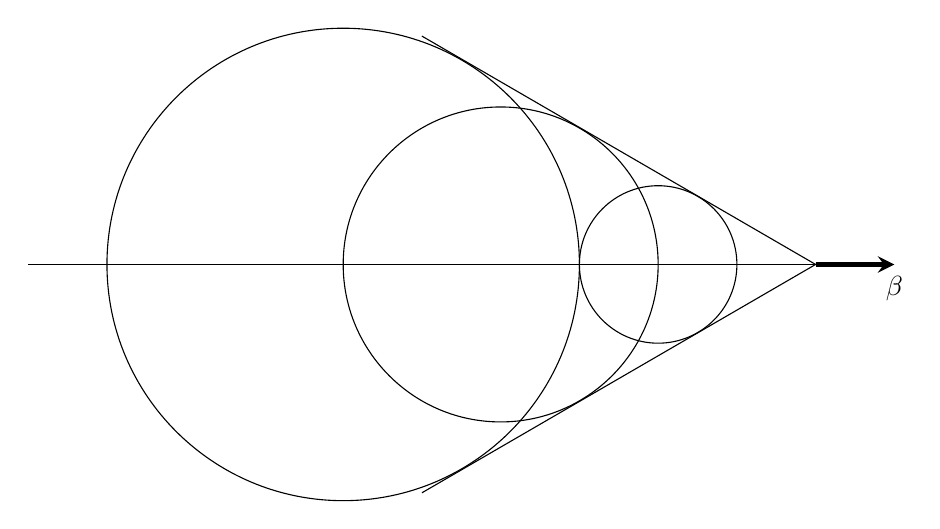
\begin{tikzpicture}
			\draw[-stealth, ultra thick](6,0)--(7,0)node[below]{$\bm\beta$};
			\draw(-4,0)--(6,0);
			\draw(6,0)--(1,2.9);
			\draw(6,0)--(1,-2.9);
			\draw (3,0) arc [start angle=0, end angle=360, x radius=3, y radius=3];
			\draw (4,0) arc [start angle=0, end angle=360, x radius=2, y radius=2];
			\draw (5,0) arc [start angle=0, end angle=360, x radius=1, y radius=1];
		\end{tikzpicture}
	\end{center}
	All'interno del cono i fronti d'onda arrivano con fasi diverse, e mediamente non viene emessa radiazione. Sul cono invece i fronti d'onda sono tutti in fase e quindi c'è radiazione. A questo punto è immediato calcolare la semiapertura del cono
	\begin{center}
		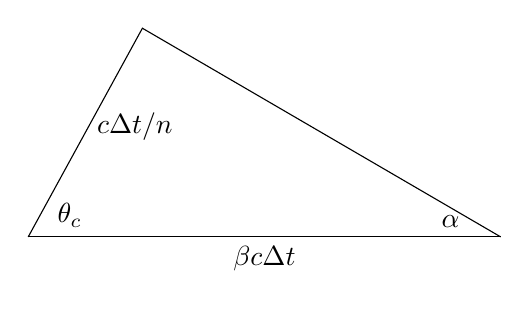
\begin{tikzpicture}
		\draw(-0,0)--(6,0);
		\draw(0,0)--(1.45,2.65)--(6,0);
		\node at(3,0)[below]{$\beta c\Delta t$};
		\node at(0.75,1.4)[right]{$c\Delta t/n$};
		\node at(5.6,0)[above left]{$\alpha$};
		\node at(0.25,0)[above right]{$\theta_c$};
		\end{tikzpicture}
	\end{center}
Alternativamente, è noto che
\[\der{I_\omega}{\Omega}\propto\left|\int_{-\infty}^{+\infty}\exp\left[i\omega\left(t-\frac{n\hat{r}\cdot\vec{v}t'}{c}\right)\right]\d t'\right|^2\propto\delta\left(\omega\left(1-\frac{nv\cos\theta}{c}\right)\right)\]
Quindi l'emissione è presente solo sul cono.
	\item\a\t{Spiegare il significato di ogni termine delle espressioni, valide per la radiazione
		Cherenkov: \begin{align*}\frac{\d^2 N_\gamma}{\d E_\gamma\d x}&= z^2 \frac{\alpha}{\hbar c}	\sin^2\theta_c\\N_\gamma &= z^2\frac{\alpha}{\hbar c}L\int_{E_1}^{E_2}\left[1-\frac{1}{\beta^2\varepsilon_r(E)}\right]P_\mathrm{det}(E)\d E
		\end{align*}} Nella prima espressione, il termine a primo membro è il numero di fotoni emesso per unità di frequenza e unità di lunghezza percorsa dalla particella (a parte un fattore $\hbar$). A secondo membro invece $z$ è la carica della particella in unità di $e$, $\alpha=e^2/\hbar c$ è la costante di struttura fine e $\theta_c$ è l'angolo mostrato nella figura precedente. Nella seconda espressione, $N_\gamma$ è il numero totale di fotoni rilevati da un detector di efficienza $P_\textrm{det}$ che può rilevare fotoni con energia compresa tra $E_1$ e $E_2$. $L$ è la lunghezza del dielettrico.
	\item\a\t{Descrivere qualitativamente le cause e gli effetti del fenomeno della radiazione di
		frenamento da parte di una particella carica nella materia.} Una particella carica che attraversa la materia interagisce con gli atomi di quest'ultima. In particolare, viene accelerata (tipicamente decelerata e deflessa), quindi perde energia per irraggiamento ed emette fotoni. In genere, le perdite per irraggiamento sono trascurabili a meno che la particella non sia un elettrone o un muone molto energetico.
	\item\a\t{Definire e dare le unità di misura di tutte le grandezze fisiche nell'espressione
		\[\der{I_\omega}{\Omega}=\frac{q^2}{4\pi^2c}\left|\int\frac{\hat{n}\wedge[(\hat{n}-\bm{\beta})\wedge\dot{\bm{\beta}}]}{(1-\hat{n}\cdot\bm{\beta})^2}\exp\left[i\omega\left(t'-\frac{\hat{n}\cdot\vec{r}'}{c}\right)\right]\d t'\right|^2\]} Vedi sezione 3, domanda 16 \b.
	\item\a\t{Definire e dare le unità di misura di tutte le grandezze fisiche nell'espressione\[I_\omega(b)=\begin{cases}
	\frac{8z^4Z^2\alpha\hbar c^2}{3\pi}\left(\frac{m_e}{M}\right)^2\frac{r_e^2}{V^2b^2}&\textrm{ }\mathrm{se}\textrm{ }\omega<V/b\\0&\textrm{ }\mathrm{se}\textrm{ }\omega>V/b
		\end{cases}\]}
	$I_\omega(b)$ è l'energia irradiata per unità di frequenza (erg$\cdot$s) in un urto coulombiano tra una particella di carica $ze$ (esu), massa $M$ (g) e velocità $V$ (cm/s) con un bersaglio fisso di carica $Ze$. $b$ è il parametro di impatto (cm), $\alpha$ la costante di struttura fine (adimensionale), $\hbar$ la costante di Planck ridotta (erg$\cdot$s), $c$ la velocità della luce (cm/s), $r_e$ e $m_e$ sono il raggio classico (cm) e la massa (g) dell'elettrone.
	\item\a\t{Definire e dare le unità di misura di tutte le grandezze fisiche nell'espressione
		\[\chi_\omega = \frac{16z^4
		Z^2\alpha\hbar c^2}{3}\left(\frac{m_e}{M}\right)^2\frac{r_e^2}{V}\ln\left[\frac{MV^2}{\hbar\omega}\right]\]}
	$\chi_\omega$ è la sezione d'urto di radiazione, definita da
	\[\chi_\omega=\int_{b_\textrm{min}}^{b_\textrm{max}}I_\omega(b)2\pi b\d b\]
	$b_\textrm{min}$ e $b_\textrm{max}$ sono rispettivamente il valore massimo e minimo che può assumere il parametro di impatto, e dipendono dalla specifica emissione che si sta studiando. Per un urto coulombiano $I_\omega$ è quella data nell'espressione precedente, $b_\textrm{max}\simeq V/\omega$ e $b_\textrm{min}\simeq\hbar/(MV)$ (quest'ultima stima è dovuta a considerazioni quantistiche). Integrando si trova l'espressione data.
	\item\a\t{Definire e dare le unità di misura di tutte le grandezze fisiche nell'espressione
		\[\der{E^\mathrm{irr}}{x}= n_\mathrm{nuclei}\frac{16}{3}z^4Z^2\alpha\left(\frac{m_e}{M}\right)^2\frac{r_e^2}{V^2}\ln \left[\frac{192}{Z^{1/3}}\frac{M}{m_e}\right]E\]} Il termine a primo membro è l'energia totale irraggiata per unità di lunghezza da una particella carica che si muove nella materia. L'espressione si ottiene integrando $n_\textrm{nuclei}\chi_\omega$ su tutte le possibili frequenze:
		\[\der{E^\textrm{irr}}{x}=n_\textrm{nuclei}\int_{0}^{\Omega}\chi_\omega\d \omega\]
		$n_\textrm{nuclei}$ è la densità di nuclei nel materiale.
\item\a\t{Dare la definizione di lunghezza di radiazione. Spiegare le condizioni per cui, nel
		caso di perdita prevalente di energia per radiazione, l’energia di una particella si
		attenua con una legge esponenziale in funzione del percorso.}
	La lunghezza di radiazione $l$ è definita da
	\[\der{E^\textrm{irr}}{x}=-\frac{E}{l}\]
	ossia
	\[l^{-1}=n_\mathrm{nuclei}\frac{16}{3}z^4Z^2\alpha\left(\frac{m_e}{M}\right)^2\frac{r_e^2}{V^2}\ln \left[\frac{192}{Z^{1/3}}\frac{M}{m_e}\right]\]
	Ovviamente, se la perdita radiativa è il canale principale per le perdite energetiche, $E$ si attenua esponenzialmente nel mezzo. Ciò accade per particelle sufficientemente energetiche, dato che
	\[\der{E^\textrm{irr}}{x}\simeq\frac{4Zz^2\alpha}{3\pi}\frac{m_e}{M}\frac{\ln\left(\frac{192}{Z^{1/3}}\frac{M}{m_e}\right)}{\ln B_q}\gamma\der{E^\textrm{coll}}{x}\]
	dove $B_q\propto\gamma mv^2$.
	\item\a\t{Spiegare tutti i termini dell'espressione \[\frac{1}{\rho X_0}= 4\alpha r_e^2 \frac{Z^2}{A(g)}N_A \left[\ln\left(\frac{184}{Z^{1/3}}\right)-f(Z)+ \frac{L'}{Z}\right]\]
		[formula di Tsai, non dimostrata a lezione] che fornisce la lunghezza di
		radiazione.} $\rho$ è la densità del materiale, $\alpha$ la costante di struttura fine, $r_e$ il raggio classico dell'elettrone, $Z$ il numero atomico, $A(g)$ la massa atomica in g, $N_A$ il numero di Avogadro, $f$ una funzione di $Z$ nella forma di una serie. Posto $a=\alpha Z$, i primi termini della serie sono
	\[f(Z)=a^2[(1+a^2)^{-1}+0.202066-0.0369a^2+0.0083a^4-0.002a^6+\dots]\]
	Infine, $L'$ dipende dal materiale e per elementi con $Z\geq5$ è
	\[L'=\ln\frac{194}{Z^{2/3}}\]
	\item\a\t{Descrivere qualitativamente il meccanismo della perdita di energia per collisioni
		da parte di una particella carica nella materia, indicando a quali entità tale energia
		viene - alla fine - trasferita e come essa possa essere misurata. Valutare l’energia
		minima e massima trasferibile in un singola collisione.} Una particella carica interagisce con gli elettroni del mezzo cedendo loro energia (si tratta di urti coulombiani). L'energia viene infine ceduta agli atomi (che si eccitano) del mezzo, e a seconda della natura di quest'ultimo si possono usare strategie diverse nella misura: per un gas, ad esempio, potrebbero essere prodotti ioni, e quindi con un campo elettrico si può registrare una corrente. In un solido, la diseccitazione può essere accompagnata dall'emissione di segnali ottici: questo fenomeno è alla base degli scintillatori (come ad esempio gli schermi fosforescenti).	
		\noindent L'energia minima trasferibile è, per motivi quantistici, l'energia corrispondente alla minima separazione tra i livelli energetici, dunque è il potenziale di prima ionizzazione $I$. Per valutare l'energia massima, consideriamo l'urto tra un elettrone di massa $m_e$ e una particella di massa $m_1$ e energia $E_1$. Sappiamo che nel centro di massa l'energia dell'elettrone è
		\[E_e^{\textrm{cm}}=\frac{M^2+m_e^2-m_1^2}{2M}\]
		dove
		\[M^2=(m_e+E_1)^2-(E_1^2-m_1^2)=m_1^2+m_e^2+2m_eE_1\]
		La velocità e il fattore di Lorentz del centro di massa sono
		\begin{align*}
			v_\textrm{cm}&=\frac{\sqrt{E_1^2-m_1^2}}{m_e+E_1}\\\gamma_\textrm{cm}&=\frac{m_e+E_1}{M}
		\end{align*}
	Dunque facendo l'opportuna trasformazione di Lorentz si ottiene
	\[E_e\geq \gamma_\textrm{cm}\left(E_e^\textrm{cm}+v_\textrm{cm}\sqrt{(E_e^\textrm{cm})^2-m_e^2}\right)=m_e\left(1+2\frac{E_1^2-m_1^2}{m_1^2+m_e^2+2m_eE_1}\right)\]
	Se poi la particella incidente è tale che $m_1^2\gg E_1m_e\gg m_e^2$, l'energia massima trasferita è
	\[T_\textrm{max}=2m_e\frac{E_1^2-m_1^2}{m_1^2+m_e^2+2m_eE_1}\simeq2m_e\gamma_1^2v_1^2\]
	\item\a\t{Spiegare il significato di ogni termine dell’espressione per la perdita di energia
		per collisioni (formula di Bethe-Bloch, non dimostrata):\[\frac{1}{\rho}\der{E^\mathrm{coll}}{x} = z^2\frac{Z}{A(g)}4\pi\frac{m_ec^2}{\beta}N_ar_e^2\left(\frac{1}{2}\ln\frac{2m_ec^2\beta^2\gamma^2}{I^2}T_\mathrm{max}-\beta^2-\frac{\delta^2}{2}\right)\]}
	Le quantità sono le stesse della formula di Tsai, a parte il potenziale di ionizzazione $I$, l'energia massima trasferibile $T_\textrm{max}$ e $\delta$, che è un fattore correttivo che limita la divergenza logaritmica per grandi $\gamma$. $\delta$ è detto fattore di densità, perchè tiene conto del fatto che il mezzo si polarizza. Il termine $-\beta^2$ invece è una correzione relativistica al calcolo classico.
	\item\a\t{Disegnare qualitativamente la funzione di Bethe-Bloch indicando i valori dei
		punti significativi.}
	\begin{figure}[h!]
		\centering
		\includegraphics[scale=0.5]{bethe.png}
	\end{figure}
L'andamento è quello riportato nella prima figura. Per bassi valori di $\beta\gamma$, la funzione diverge come $1/\beta^2$. Il minimo si trova per $\beta\gamma\simeq 3.5$ e vale approssimativamente 2 MeV/(g/cm$^2$). Per alti valori di $\beta\gamma$, la correzione sulla densità limita la crescita della funzione. In realtà, un grafico più realistico per la perdita di energia non diverge quando $\beta\to0$, anzi in genere ha un massimo per $\beta\gamma\sim0.01$. Questo andamento è dovuto a interazioni con i nuclei. Viceversam per $\beta\gamma$ molto elevato (tipicamente intorno a 1000) le perdite radiative diventano importanti e dominano sulle perdite collisionali, che per la correzione di densità hanno una sorta di plateau. Un grafico più realistico è quindi il secondo.
\begin{figure}[h!]
	\centering
	\includegraphics[scale=0.4]{bethe2.png}
\end{figure}
	\item\a\t{Definire il "percorso residuo" ("range") per una particella carica in un materiale.} Il percorso residuo è lo spazio percorso dalla particella prima di fermarsi. Se questa ha energia cinetica $T$, si ha semplicemente
	\[R(T)=\int_{0}^{T}\left|\der{E}{x}\right|^{-1}\d E\]
	\item\a\t{Dare la definizione di "Energia critica".} L'energia critica $E_c$ è il valore dell'energia per cui le perdite collisionali e radiative sono uguali, ovvero
	\[\der{E^\textrm{coll}}{x}(E_c)=\der{E^\textrm{irr}}{x}(E_c)\]
	\item\a\t{Descrivere qualitativamente il fenomeno dello scattering multiplo da parte di una
		particella carica in moto veloce nella materia. Valutare il rapporto fra angolo
		minimo e massimo in una singola collisione.} Nell'urto di una particella con un atomo bersaglio, è assai improbabile che l'angolo di deflessione sia molto grande. Se la particella attraversa la materia, ci aspettiamo che faccia molti urti con gli atomi del mezzo, ciascuno con piccole deflessioni. Il teorema del limite centrale ci assicura che nel limite di numerose interazioni l'angolo di deflessione è distribuito gaussianamente. Se l'angolo di scattering è piccolo, è noto che
	\[\theta\simeq\frac{2ze^2}{pvb}\]
	Posto
	\[a=1.4\frac{a_0}{Z^{1/3}}\]
	si ha
	\[\theta_\textrm{min}\simeq\frac{2ze^2}{pva}\]
	Se invece si vogliono fare considerazioni quantistiche, si ha
	\[\theta^q_\textrm{min}\simeq\frac{\hbar}{pa}\simeq\frac{Z^{1/2}}{192}\frac{m_ec}{p}\]
	Per stimare l'angolo massimo, posto
	\[R=1.4A^{1/3}\textrm{ fm}\]
	si può stimare
	\[\theta_\textrm{max}\simeq\frac{\hbar}{pR}\simeq\frac{274}{A^{1/2}}\frac{m_ec}{p}\]
	e dunque
	\[\frac{\theta_\textrm{min}}{\theta_\textrm{max}}\simeq\frac{274 Z^{1/2}}{192 A^{1/2}}\simeq1\]
	\item\a\t{Definire l'angolo di multiplo scattering (rispetto alla direzione iniziale della
		particella) e definire la sua proiezione su un piano (che contiene la direzione
		iniziale della particella). Indicare i limiti delle due variabili cosí definite.}
	L'angolo di multiplo scattering rappresenta l'angolo compreso tra la direzione di moto iniziale e finale di una particella che attraversa uno strato di materia. Può essere interessante proiettare questo angolo su un qualche piano particolare.
	\item\a\t{Spiegare il significato di ogni termine dell'espressione per l’angolo quadratico
		medio di multiplo scattering (rispetto alla direzione iniziale della particella)
		\[\sqrt{\langle\theta^2_{\mathrm{ms}}\rangle}=\theta_0\sqrt{2}= z
		\frac{13.6\mathrm{MeV}}{P\beta c}\sqrt{\frac{L}{X_0}}\left(1+0.0038\ln\frac{L}{X_0}\right)\sqrt{2}\]}
	$P$ è l'impulso iniziale della particella, $\beta c$ la sua velocità, $L$ lo spessore di materiale attraversato, $X_0$ la lunghezza di radiazione del materiale.
	\item\a\t{Illustrare in modo qualitativo il metodo di produzione degli antiprotoni
		nell’esperimento di Segré et al. ed il principio della loro rivelazione.} L'apparato sperimentale è nella figura successiva
	\clearpage
	\begin{figure}[h]
		\centering
		\includegraphics[scale=0.5]{bevatron.png}
	\end{figure}

	Un fascio di protoni del Bevatron colpisce un bersaglio di rame e genera particelle con carica negativa di impulso $p=1.19$ MeV/c. Le particelle possono essere antiprotoni o pioni, con circa 1 antiprotone ogni $10^5$ pioni. Inoltre, con quell'impulso si ha $\beta=0.99$ per i pioni e $\beta=0.78$ per gli antiprotoni. Le particelle sono deflesse di 21$^\circ$ dal campo magnetico del Bevatron e di $34^\circ$ aggiuntivi dal magnete M1. Attraversano poi Q1, un magnete quadrupolare usato per focalizzare il fascio. Analogamente, Q2 è un altro magnete quadrupolare che focalizza il fascio e M2 un magnete che deflette le particelle di altri 34$^\circ$. S1, S2 e S3 sono scintillatori ordinari, C1 è un contatore Cerenkov che rivela tutte le particelle cariche con $\beta>0.79$. C2 è un contatore Cerenkov che rivela tutte le particelle cariche con $0.75<\beta<0.78$. S3 è uno scintillatore usato per evitare che le particelle che attraversano C2 non abbiano angoli di scattering troppo grossi. Inoltre, S1 e S2 distano 40 ft, dunque è possibile misurare la velocità delle particelle anche in un secondo modo. In tal modo si riesce a distinguere tra antiprotoni e pioni, e misurando la velocità e l'impulso degli antiprotoni si può anche confrontare la massa di questi con la massa del protone.
	\item\a\t{Descrivere l’esperimento di Anderson sulla scoperta del positrone.}
	Nell'esperimento venne usata una camera a nebbia, ossia un dispositivo isolato contenente del vapore saturo. Una particella carica e sufficientemente energetica che attraversa la camera ionizza il gas sulla sua traiettoria e gli atomi ionizzati formano dei nuclei di condensazione su cui cominciano a formarsi delle goccioline. Fotografando la camera è possibile ricostruire la traiettoria della particella incidente. Se poi la camera è immersa in un campo magnetico, è possibile misurare l'impulso della particella a partire dal raggio di curvatura. Nell'esperimento di Anderson venne registrata la traccia di una particella che attraversa uno strato di piombo di 6 mm. Prima dello strato la particella aveva $p_i=63$ MeV/c, dopo $p_f=22.5$ MeV/c.
	\begin{figure}[h!]
		\centering
		\includegraphics[scale=0.3]{anderson.jpg}
	\end{figure}
	Dal verso della curvatura della traiettoria si deduce che la particella ha carica positiva. L'unica particella positiva nota al tempo era il protone, ma con quell'impulso il protone è non relativistico. La perdita di energia per ionizzazione è molto elevata e il range è di circa 5 mm, quindi un protone con quell'impulso non può attraversare uno strato di piombo di 6 mm. Se invece assumiamo che la particella sia un positrone, deve essere ultrarelativistico sia prima che dopo aver attraversato la lastra. Dato che questa è spessa quanto una lunghezza di radiazione, l'energia del positrone emergente è
	\[E_f=\frac{E_i}{e}=23\textrm{ MeV}\]
	Quindi è compatibile con il valore misurato.
\end{enumerate}
\begin{enumerate}
	\item\b\t{Dimostrare che all’interno del cono della radiazione Cherenkov vi sono due
		soluzioni per $t' = t - nR/c$, nessuna soluzione all’esterno, ed una sola sul fronte
		d’onda.} Prendiamo una particella che si muove di moto rettilineo uniforme con velocità $\vec{v}=v\hat{z}$. La definizione di tempo ritardato è
	\[c(t-t')=n|\vec{x}-\vec{v}t'|\]
	Posto $r^2=x^2+y^2$, si ottiene
	\[t'^2\left(1-\frac{c^2}{n^2v^2}\right)-2t'\left(\frac{z}{v}-\frac{c^2t}{n^2v^2}\right)+\frac{r^2+z^2}{v^2}-\frac{c^2t^2}{n^2v^2}=0\]
	A meno di costanti moltiplicative positive, il discriminante è
	\[\Delta\propto(z-vt)^2-r^2\left(\frac{n^2v^2}{c^2}-1\right)\]
	In particolare, è positivo se
	\[\sin\theta:=\frac{r}{\sqrt{r^2+(z-vt)^2}}<\frac{c}{nv}\]
	In tal caso esistono due soluzioni distinte per il tempo ritardato. Se invece si impone l'uguaglianza (ossia se siamo sul cono) esiste una sola soluzione, mentre se si impone l'altra disuguaglianza non esistono soluzioni. Si noti che
	\[t-t'=\frac{t}{1-\frac{c^2}{n^2v^2}}-\frac{z}{v}\frac{1}{1-\frac{c^2}{n^2v^2}}\pm\frac{\frac{c}{nv^2}}{1-\frac{c^2}{n^2v^2}}\sqrt{(z-vt)^2-\left(\frac{n^2v^2}{c^2}-1\right)r^2}\]
	Se $v>c/n$ e $z<vt$ entrambe le radici sono positive, mentre se $z>vt$ entrambe le radici sono negative, quindi effettivamente si hanno due tempi ritardati all'interno del cono, nella falda "dietro" la particella, un solo tempo ritardato sulla superficie del cono e nessuna soluzione all'esterno del cono e nella falda "davanti" alla particella.
	\item\b\t{A partire dalla espressione 
		\[\frac{\d ^2N_\gamma}{\d E_\gamma \d x}=z^2\frac{\alpha}{\hbar c}\sin^2\theta_c\] valida per la radiazione Cherenkov,		dimostrare che \[N_\gamma=z^2\frac{\alpha
		}{\hbar c}L\int_{E_1}^{E_2}\left[1-\frac{1}{\beta^2\varepsilon_r(E)}\right]P_\mathrm{det}(E)\d E\]}
		Basta ricordare che
		\[\sin^2\theta_c=1-\frac{c^2}{n^2(E)v^2}=1-\frac{1}{\beta^2\varepsilon_r(E)}\]
		e fare una banale integrazione su $E_\gamma$ e su $x$.
	\item\b\t{Calcolare il numero di fotoni osservati da un fotorivelatore sensibile con
		efficienza del 30\% a luce fra 300 $\mathrm{nm}$ e 600 $\mathrm{nm}$, al passaggio di un elettrone nei due
		casi seguenti: i) n=1.005 (gas), $\beta$=0.999, lunghezza=1 $\mathrm{m}$; ii) n=1.5 (solido
		trasparente), $\beta$=0.99, lunghezza=1 $\mathrm{cm}$.}
	In generale, per un fotorivelatore con efficienza costante tra le frequenze $\omega_1$ e $\omega_2$ e per un mezzo non dispersivo in tale banda di frequenze, si ottiene
	\[N_\gamma=z^2\frac{\alpha}{c}L(\omega_2-\omega_1)\left(1-\frac{1}{\beta^2n^2}\right)P_\textrm{det}\]
	Passando alle lunghezze d'onda
	\[N_\gamma=2\pi z^2\alpha L\left(\frac{1}{\lambda_2}-\frac{1}{\lambda_1}\right)\left(1-\frac{1}{\beta^2n^2}\right)P_\textrm{det}\]
	Nei due casi proposti si ottiene $N_\gamma=91$ e $N_\gamma=74$.
	\item\b\t{Calcolare l’angolo di emissione della radiazione Cherenkov in funzione
		dell’impulso (e della massa) della particella e dell’indice di rifrazione.}
	\[\sin\theta_c=\frac{1}{n\beta}=\frac{1}{n}\sqrt{1+\left(\frac{mc}{p}\right)^2}\]
	\item\b\t{Descrivere qualitativamente il principio di funzionamento dei rivelatori
		Cherenkov: i) a soglia, ii) RICH, iii) DIRC.} Un contatore a soglia è composto in genere da un radiatore, ossia da un mezzo trasparente (ad esempio, propano sotto pressione) in cui può essere generata radiazione Cherenkov, uno specchio sferico o parabolico e un rivelatore di fotoni. Una particella veloce che attraversa il mezzo emette radiazione Cherenkov, che viene deviata dallo specchio e raccolta dal rivelatore (o anche da un fotomoltiplicatore, visto che in genere il numero di fotoni emessi non è molto elevato). Un contatore a soglia può quindi discriminare le particelle che attraversano il radiatore a seconda che $\beta$ sia maggiore o minore di $n^{-1}$, quindi è utile per separare, in un fascio con un dato impulso, particelle di massa diversa. In un rivelatore RICH (Ring Imaging CHerenkov counter), si usa un radiatore piuttosto sottile, dietro al quale è posto un piano fotosensibile. In tal modo, è possibile ricostruire anche la posizione in cui vengono rivelati i singoli fotoni: la figura che si forma è un cerchio, e dalla misura del suo raggio e dalla distanza dal radiatore è possibile ricostruire l'angolo del cono di radiazione. Infine, in un rivelatore DIRC (Detector for Internal Reflected Cherenkov light), il radiatore è composto da barre di quarzo, che fungono anche da guida d'onda. Infatti, quando una particella attraversa il quarzo ed emette radiazione Cherenkov è possibile che avvenga riflessione totale. In tal modo, l'angolo del cono Cherenkov e la polarizzazione sono conservati fino alle estremità della barra, dove opportuni rivelatori sono in grado di registrare il passaggio della particella e misurare l'angolo di apertura del cono.
	\item\b\t{Partendo dalla espressione
		\[\der{I_\omega}{\Omega}=\frac{q^2}{4\pi^2c}\left|\int\frac{\hat{n}\wedge[(\hat{n}-\bm{\beta})\wedge\dot{\bm{\beta}}]}{(1-\hat{n}\cdot\bm{\beta})^2}\exp\left[i\omega\left(t'-\frac{\hat{n}\cdot\vec{r}'}{c}\right)\right]\d t'\right|^2\]
		dimostrare che
		l’energia persa per unita’ di frequenza nel caso non relativistico e’ approssimabile
		con \[I_\omega=\begin{cases}
		\frac{2q^2}{3\pi c}\left|\Delta\bm{\beta}\right|&\textrm{ }\mathrm{se}\textrm{ }\omega<1/\tau\\0&\textrm{ }\mathrm{se}\textrm{ }\omega>1/\tau
		\end{cases}\]} Nel caso non relativistico si può approssimare
	\[\der{I_\omega}{\Omega}\simeq\frac{q^2}{4\pi^2c}\left|\int\hat{n}\wedge(\hat{n}\wedge\dot{\bm\beta})e^{i\omega t'}\d t'\right|^2\]
	Detto $\tau$ il tempo tipico in cui la carica è accelerata, distinguiamo due regimi. Se $\omega\tau\ll 1$ si ottiene, approssimando ulteriormente
	\[\der{I_\omega}{\Omega}\simeq\frac{q^2}{4\pi^2c}\left|\int\hat{n}\wedge(\hat{n}\wedge\dot{\bm\beta})\d t\right|^2=\frac{q^2}{4\pi^2 c}|\Delta\bm\beta|^2\sin^2\theta\]
	dove $\theta$ è l'angolo tra $\Delta\bm\beta$ e $\hat{n}$. Intengrando sull'angolo solido si ottiene
	\[I_\omega=\frac{2q^2}{3\pi c}|\Delta\bm\beta|^2\]
	Nel limite opposto $\omega\tau\gg1$ l'energia irraggiata è trascurabile per il lemma di Riemann-Lebesgue. 
	\item\b\t{Partendo dalla espressione
		\[\der{I_\omega}{\Omega}=\frac{q^2}{4\pi^2c}\left|\int\frac{\hat{n}\wedge[(\hat{n}-\bm{\beta})\wedge\dot{\bm{\beta}}]}{(1-\hat{n}\cdot\bm{\beta})^2}\exp\left[i\omega\left(t'-\frac{\hat{n}\cdot\vec{r}'}{c}\right)\right]\d t'\right|^2\]
		dimostrare che
		l’energia persa per unità di frequenza nel caso non relativistico ad un dato
		parametro di impatto $b$ e’ approssimabile con \[I_\omega(b)=\begin{cases}
		\frac{8z^4Z^2\alpha\hbar c^2}{3\pi}\left(\frac{m_e}{M}\right)^2\frac{r_e^2}{V^2b^2}&\textrm{ }\mathrm{se}\textrm{ }\omega<V/b\\0&\textrm{ }\mathrm{se}\textrm{ }\omega>V/b
		\end{cases}\]}
		Facendo i calcoli precedenti si ottiene
		\[I_\omega=\begin{cases}
		\frac{2q^2}{3\pi c}\left|\Delta\bm{\beta}\right|&\textrm{ }\mathrm{se}\textrm{ }\omega<1/\tau\\0&\textrm{ }\mathrm{se}\textrm{ }\omega>1/\tau
		\end{cases}\]
		Nel caso di urto coulombiano, il tempo tipico di collisione è $b/V$. Calcoliamo adesso $\Delta\bm\beta$. Per piccoli angoli di scattering e in approssimazione non relativistica si ha
		\[Mc\Delta\bm\beta=zZe^2\hat{y}\int_{-\infty}^{+\infty}\frac{b}{(V^2t^2+b^2)^{3/2}}\d t=\frac{2zZe^2}{bV}\]
		Da cui, per $\omega<V/b$,
		\[I_\omega=\frac{8z^4Z^2\alpha\hbar c^2}{3\pi}\left(\frac{m_e}{M}\right)^2\frac{r_e^2}{V^2b^2}\]
	\item\b\t{Dimostrare, a partire dalla espressione precedente, che la sezione d’urto di
		irraggiamento non relativistica e' approssimabile con \[\chi_\omega=\frac{16z^4Z^2\alpha\hbar c^2}{3}\left(\frac{m_e}{M}\right)^2\frac{r_e^2}{V^2}\ln\left[\frac{MV^2}{\hbar\omega}\right]\]}
	Per definizione si ha
	\[\chi_\omega=2\pi\int_{b_\textrm{min}}^{b_\textrm{max}}I_\omega b\,\d b=\frac{16z^4Z^2\alpha\hbar c^2}{3}\left(\frac{m_e}{M}\right)^2\frac{r_e^2}{V^2}\ln\frac{b_\textrm{max}}{b_\textrm{min}}\]
	Dobbiamo solo esplicitare gli estremi di integrazione. Per l'estremo superiore, basta ricordare che deve essere $\omega<V/b$, quindi
	\[b_\textrm{max}=\frac{V}{\omega}\]
	L'estremo inferiore si ottiene con considerazioni quantistiche (essenzialmente con il principio di indeterminazione, $b_\textrm{min}$ viene scelto in modo che abbia senso parlare di traiettoria), e vale
	\[b_\textrm{min}=\frac{\hbar}{MV}\]
	\item\b\t{Dimostrare che nel caso relativistico la sezione d’urto di irraggiamento e'
		approssimabile, in un modello, con \[\chi_\omega=\frac{16}{3}z^4Z^2\alpha r_e^2\left(\frac{m_e}{M}\right)^2\hbar\ln\left(\frac{192}{Z^{1/3}}\frac{M}{m_e}\right)\] per
		$\omega < (\gamma-1)Mc^2/\hbar$.}
	Poniamo nel sistema inizialmente in quiete con la particella incidente. In questo sistema il suo moto rimane non relativistico, dunque
	\[\chi'_{\omega'}=\frac{16z^4Z^2\alpha\hbar c^2}{3}\left(\frac{m_e}{M}\right)^2\frac{r_e^2}{V^2}\ln\frac{b_\textrm{max}}{b_\textrm{min}}\]
	$b_\textrm{min}$ rimane lo stesso (essenzialmente perchè tutti i punti della particella incidente debbono muoversi con la stessa accelerazione), dunque
	\[b_\textrm{min}=\frac{\hbar}{MV}\]
	In linea di principio, l'altro estremo è $b_\textrm{max}=\gamma V/\omega'$ a causa della dilatazione dei tempi. Tuttavia, si deve anche tener conto del fatto che le cariche elettroniche schermano la carica nucleare se ci troviamo a una distanza
	\[b_s=1.4\frac{a_0}{Z^{1/3}}\]
	Dunque poniamo
	\[b_\textrm{max}=\min\left\{\frac{\gamma V}{\omega},b_s\right\}\]
	e per particelle relativistiche ovviamente scegliamo $b_s$. A questo punto si ricordi che
	\[a_0=\frac{\hbar}{m_ec\alpha}\simeq\frac{137\hbar}{m_ec}\]
	da cui si ottiene infine
	\[\chi'_{\omega'}=\frac{16z^4Z^2\alpha\hbar c^2}{3}\left(\frac{m_e}{M}\right)^2\frac{r_e^2}{V^2}\ln\frac{192}{Z^{1/3}}\frac{MV}{m_ec}\]
	$\chi_\omega$ è un'invariante di Lorentz, dato che è il prodotto (energia)$\cdot$(area traversa)/(frequenza): energia e frequenza trasformano allo stesso modo, un'area trasversa è invariante. Notando ulteriormente che $V\simeq c$, si ottiene
	\[\chi_\omega=\frac{16}{3}z^4Z^2\alpha r_e^2\left(\frac{m_e}{M}\right)^2\hbar\ln\left(\frac{192}{Z^{1/3}}\frac{M}{m_e}\right)\]
	La conservazione dell'energia richiede poi $\hbar\omega<(\gamma-1)Mc^2$.
	
	\item\b\t{Dimostrare che nel caso relativistico la perdita di energia per irraggiamento e'
		approssimabile con
		\[\der{E^\mathrm{irr}}{x}= n_\mathrm{nuclei}\frac{16}{3}z^4Z^2\alpha\left(\frac{m_e}{M}\right)^2\frac{r_e^2}{V^2}\ln \left[\frac{192}{Z^{1/3}}\frac{M}{m_e}\right]E\]}
	Per attraversare un tratto $\d x$, la particella perde un'energia alla frequenza $\omega$ pari a \[\d E^\textrm{irr}=n_\textrm{nuclei}\chi_\omega\d x\]
	Si trova dunque
	\[\der{E^\textrm{irr}}{x}=n_\textrm{nuclei}\int_{0}^{(\gamma-1)Mc^2\hbar^{-1}}\chi_\omega\d \omega= n_\mathrm{nuclei}\frac{16}{3}z^4Z^2\alpha\left(\frac{m_e}{M}\right)^2\frac{r_e^2}{V^2}\ln \left[\frac{192}{Z^{1/3}}\frac{M}{m_e}\right](\gamma-1)Mc^2\]
	Basta ora notare che per particelle relativistiche $(\gamma-1)Mc^2\simeq E$.
	\item\b\t{Valutare la lunghezza di radiazione del Piombo e del Silicio utilizzando il modello
		utilizzato e confrontarla con i valori sperimentali.}
	Usando la formula di Tsai con $f(Z)\simeq (\alpha Z)^2/(1+a(\alpha Z)^2)$, si ottiene
	\begin{align*}X_{0,\textrm{Pb}}&\simeq0.56\textrm{ cm}\\X_{0,\textrm{Si}}&\simeq9.85\textrm{ cm}\end{align*}
	I valori sperimentali sono invece
	\begin{align*}X_{0,\textrm{Pb}}&\simeq0.56\textrm{ cm}\\X_{0,\textrm{Si}}&\simeq9.4\textrm{ cm}\end{align*}
	\item\b\t{Calcolare l'energia irraggiata da un elettrone di 60 $\mathrm{MeV}$ che attraversi 5.6 $\mathrm{mm}$ di
		Pb e calcolare il numero medio di fotoni emessi di energia fra 1 $\mathrm{eV}$ e 1 $\mathrm{MeV}$.}
	Dato che lo spazio percorso è la lunghezza di radiazione, l'energia irraggiata è
	\[E^\textrm{irr}=E(1-e^{-1})\simeq38\textrm{ MeV}\]
	Il numero di fotoni emessi per unità di lunghezza e di frequenza è $\chi_\omega/(\hbar\omega)$, dunque i fotoni emessi tra le energie $E_1$ ed $E_2$ sono
	\[N_\gamma=\frac{16}{3}X_0Z^2\alpha r_e^2\ln\frac{192}{Z^{1/3}}\frac{M}{m_e}\ln\frac{E_2}{E_1}\]
	\item\b\t{Calcolare il numero medio di fotoni emessi di energia fra 10 e 100 $\mathrm{MeV}$ per un
		elettrone di 1 $\mathrm{GeV}$ che attraversi 300 $\mu\mathrm{m}$ di Silicio o 1 $\mathrm{mm}$ di Piombo. Calcolare
		poi la probabilità che uno di questi fotoni effettui una interazione prima di uscire
		dal materiale.}
	Il calcolo è lo stesso, a patto di sostituire $X_0$ con lo spessore $\Delta l$ attraversato. La probabilità di interazione è infine
	\[P=\frac{\rho N_A}{A}\sigma\frac{\Delta l}{2}\]
	Il fattore 2 è stato introdotto immaginando che i fotoni siano emessi a metà dello spessore.
	\item\b\t{Utilizzando le tabelle che forniscono le sezioni d'urto di fotoni su atomi, calcolare
		la probabilita' che un fotone da 10 $\mathrm{MeV}$ produca una coppia $e^+e^-$ in uno spessore
		di Piombo pari ad una lunghezza di radiazione.} I calcoli sono quelli precedenti, la sezione d'urto a quella energia per la produzione di coppie è
	\[\sigma\simeq0.1\textrm{ b}\]
	da cui
	\[P\simeq1.8\cdot10^{-3}\]
	\item\b\t{Indicare le ipotesi effettuate e dimostrare la seguente espressione, approssimata,
		per la perdita di energia per collisioni (formula di Bohr):
		\[\frac{1}{\rho}\der{E_\mathrm{coll}}{x}=z^2\frac{Z}{A(g)}4\pi\frac{m_ec^2}{\beta^2}N_Ar_e^2\ln\frac{c\beta^3\gamma^2}{z\omega_er_e}\]
	} Consideriamo un urto coulombiano tra una particella di massa $m\gg m_e$, in moto non relativistico. Trascuriamo lo schermaggio e l'interazione con il nucleo, di modo che La variazione di impulso in un singolo urto con un elettrone sia stimabile con
\[\Delta p=\frac{2ze^2}{vb}=\frac{2zr_em_ec^2}{vb}\]
L'approssimazione è vera se l'angolo di scattering è piccolo, di modo da poter considerare la traiettoria della particella pressochè rettilinea, e se la durata della collisione è piccola rispetto al periodo di rotazione dell'elettrone intorno al nucleo, di modo da considerare l'elettrone libero e inizialmente a riposo. L'energia persa dalla particella è allora
\[\Delta\mathcal{E}=\frac{(\Delta p)^2}{2m_e}=\frac{2z^2r_e^2m_ec^2}{\beta^2b^2}\]
Detta $\rho$ la densità del materiale, $A(g)$ la massa di un atomo in g e $Z$ il numero atomico, la densità di elettroni è
\[n_e=\frac{\rho ZN_A}{A(g)}\]
Dunque si ottiene
\[\frac{1}{\rho}\der{E_\textrm{coll}}{x}=\frac{ZN_A}{A(g)}\int_{b_\textrm{min}}^{b_\textrm{max}}2\pi\mathcal{E}b\,\d b=z^2\frac{Z}{A(g)}4\pi\frac{m_ec^2}{\beta^2}N_Ar_e^2\ln\frac{b_\textrm{max}}{b_\textrm{min}}\]
Dette $T_\textrm{min}$ e $T_\textrm{max}$ rispettivamente l'energia massima e minima trasferibili all'elettrone, si ha a meno di segni
\[\ln\frac{b_\textrm{max}}{b_\textrm{min}}=\frac{1}{2}\ln\frac{T_\textrm{max}}{T_\textrm{min}}\]
Valutiamo ora le due energie. Come noto, si ha
\[T_\textrm{max}=2m_e\gamma^2v^2\]
Per l'energia minima, ricordiamo che deve essere $\omega_e\tau\ll1$, dove $\omega_e$ è la frequenza tipica dell'elettrone intorno al nucleo e $\tau$ è il tempo tipico di collisione. Dato che $\tau=b/(\gamma v)$, si ottiene
\[T_\textrm{min}=\frac{2z^2r_e^2m_ec^2}{M^2\beta^2b_\textrm{max}^2}=\frac{2z^2r_e^2m_e\omega_e^2}{\gamma^2\beta^4}\]
da cui infine
\[\frac{1}{\rho}\der{E_\mathrm{coll}}{x}=z^2\frac{Z}{A(g)}4\pi\frac{m_ec^2}{\beta^2}N_Ar_e^2\ln\frac{c\beta^3\gamma^2}{z\omega_er_e}\]
	\item\b\t{Utilizzando la modellizzazione $I = (16\mathrm{eV})\cdot Z^{0.9}$, valutare il valore minimo
		dell’energia persa per collisioni, in $\mathrm{MeV/g/cm}^2$, per i seguenti materiali: i)
		Piombo, ii) Silicio; iii) aria a TPN.}
	Prendiamo la formula di Bethe-Bloch, trascurando le correzioni e inserendo $I=(16\textrm{ eV})\cdot Z^{0.9}$
	\[\frac{1}{\rho}\der{E^\mathrm{coll}}{x} = z^2\frac{Z}{A(g)}4\pi\frac{m_ec^2}{\beta^2}N_ar_e^2\ln\frac{2m_ec^2\beta^2\gamma^2}{(16\textrm{ eV})\cdot Z^{0.9}}\]
	Come noto il minimo si ha per $\gamma\beta\simeq 3.5$, da cui per gli elettroni
	\begin{align*}\frac{1}{\rho}\left.\der{E^\textrm{coll}}{x}\right|_{\textrm{min}}&=0.303\frac{Z}{A(g)}\ln\left(\frac{7.8\cdot 10^{5}}{Z^{0.9
	}}\right)\textrm{ MeV/g/cm}^2=\\&=\left(4.11-0.27\ln Z\right)\frac{Z}{A(g)}\textrm{ MeV/g/cm}^2\end{align*}
	Volendo essere ancora più brutali, $A\simeq 2Z$, dunque
	\begin{align*}\frac{1}{\rho}\left.\der{E^\textrm{coll}}{x}\right|_{\textrm{min}}&=\left(2.08-0.135\ln Z\right)\textrm{ MeV/g/cm}^2\end{align*}
	Nei casi richiesti si ottiene
	\begin{align*}
		\frac{1}{\rho}\left.\der{E^\textrm{coll}}{x}\right|_{\textrm{min, Pb}}&=1.15\textrm{ MeV/g/cm}^2\\
		\frac{1}{\rho}\left.\der{E^\textrm{coll}}{x}\right|_{\textrm{min, Si}}&=1.69\textrm{ MeV/g/cm}^2\\
		\frac{1}{\rho}\left.\der{E^\textrm{coll}}{x}\right|_{\textrm{min, aria}}&=1.7\textrm{ MeV/g/cm}^2
	\end{align*}
	\item\b\t{Scrivere l'espressione per calcolare il "percorso residuo" ("range"), nota la curva
		$\d E_\mathrm{coll}/\d x$, in funzione dell'energia della particella.} Vedi 4.17(a).
	\item\b\t{Calcolare nel caso relativistico l’energia in cui la perdita di energia per
		irraggiamento e’ paragonabile a quella per collisioni in funzione della massa della
		particella. Determinare il valore per elettroni e protoni nel Piombo o in aria.}
	Per particelle relativistiche ($\beta\simeq1$) con $z=\pm1$, il valore critico del fattore di Lorentz è definito implicitamente da
	\[\gamma_c=\frac{3\pi}{4\alpha Z}\frac{M}{m_e}\frac{\ln\frac{2m_ec^2\gamma_c^2}{I}}{\ln\frac{192}{Z^{1/3}}\frac{M}{m_e})}\]
	Usando la modellizzazione $I=(16\textrm{ eV})\cdot Z^{0.9}$, si ottiene
	\[\gamma_c\simeq\frac{323}{Z}\frac{M}{m_e}\frac{2\ln\gamma_c+11}{\ln\frac{M}{m_e}+5.26}\]
	dove si è trascurata la dipendenza logaritmica da $Z$. Numericamente, per elettroni nel piombo si trova $\gamma_c\simeq 11.9$ (sperimentalmente si misura $\gamma_c=15.6$), mentre in aria $\gamma_c\simeq88$. Per protoni nel piombo si trova $\gamma_c\simeq1.7\cdot10^4$, in aria $\gamma_c\simeq1.1\cdot10^5$.
	\item\b\t{Nell'approssimazione di piccoli angoli e distribuzione gaussiana, calcolare il valor
		medio, il valore quadratico medio e la sigma per: i) l'angolo di multiplo scattering
		rispetto alla direzione iniziale della particella, e ii) la sua proiezione su un piano
		che contenga la direzione iniziale della particella.}
		Assumiamo che la particella si muova inizialmente lungo l'asse $\hat{z}$. Sia $\theta$ l'angolo di multiplo scattering e $\theta_x,\theta_y$ le sue proiezioni sui piani $xz$ e $yz$. Se assumiamo che $\theta_x$ e $\theta_y$ siano distributi gaussianamente, per simmetria devono avere la stessa deviazione standard e media nulla, ossia
		\[P(\theta_x)=\frac{1}{\theta_0\sqrt{2\pi}}e^{-\frac{\theta_x^2}{2\theta_0^2}}\]
		e analogo per $P(\theta_y)$. Ovviamente si ha
		\begin{align*}
			\langle\theta_x\rangle&=\langle\theta_y\rangle=0\\\langle\theta_x^2\rangle&=\langle\theta_y^2\rangle=\theta_0^2\\\sigma_{\theta_x}&=\sigma_{\theta_y}=\theta_0
		\end{align*}
		Passiamo alla distribuzione di $\theta$. Si ha $\theta^2=\theta_x^2+\theta_y^2$, inoltre la condizione di normalizzazione su $\theta_x$ e $\theta_y$ implica
		\begin{align*}
			1&=\int_{-\infty}^{+\infty}\d \theta_x\int_{-\infty}^{+\infty}\d \theta_yP(\theta_x)P(\theta_y)=\\&=
			\int_{-\infty}^{+\infty}\d \theta_x\int_{-\infty}^{+\infty}\d \theta_y\frac{1}{2\pi\theta_0^2}\exp\left(-\frac{\theta_x^2+\theta_y^2}{2\theta_0^2}\right)=\\&=\int_{0}^{+\infty}\frac{\theta}{\theta_0^2}e^{-\frac{\theta^2}{2\theta_0^2}}\d \theta
		\end{align*}
		La funzione
		\[\mathcal{P}(\theta)=\frac{\theta}{\theta_0^2}e^{-\frac{\theta^2}{2\theta_0^2}}\]
		è la funzione con cui è distribuito $\theta$ ed è nota come distribuzione di Molière. A questo punto con semplici calcoli
		\begin{align*}
			\langle\theta\rangle&=\int_{0}^{+\infty}\frac{\theta^2}{\theta_0^2}e^{-\frac{\theta^2}{2\theta_0^2}}\d \theta=\theta_0\sqrt{\frac{\pi}{2}}\\\langle\theta^2\rangle&=\int_{0}^{+\infty}\frac{\theta^3}{\theta_0^2}e^{-\frac{\theta^2}{2\theta_0^2}}\d \theta=2\theta_0^2\\\sigma_\theta&=\sqrt{\langle\theta^2\rangle-\langle\theta\rangle^2}=\theta_0\sqrt{\frac{4-\pi}{2}}
		\end{align*}
	Si noti che $\theta_0$ è il massimo di $\mathcal{P}$.
	\item\b\t{Se non fosse sufficiente la approssimazione di piccoli angoli e distribuzione
		gaussiana, indicare quale fra le seguenti funzioni descriverebbe la distribuzione 
		che meglio descrive il fenomeno del multiplo scattering: i) Bethe-Bloch, ii)
		Moliere, iii) Breit-Wigner, iv) Bohr.} Moliere.
	\item\b\t{Dimostrare l'espressione approssimata per l’angolo quadratico medio di multiplo
		scattering (proiezione su un piano): \[\theta_0=z\frac{\mathrm{cost.}}{P\beta c}\sqrt{\frac{L}{X_0}}\]
		e confrontare il valore dela
		costante ottenuta con la formula contenuta nel PDG.}
	Prendiamo la sezione d'urto Mott, trascurando il termine con $\beta$:
	\[\der{\sigma_m}{\Omega}=\left(\frac{zZr_em_ec^2}{2Pv}\right)^2\frac{1}{\sin^4\frac{\theta}{2}}\]
	Dato che l'angolo di scattering $\theta_s$ nel singolo urto è molto piccolo, la sezione d'urto è
	\[\sigma_{m,s}\simeq2\pi\left(\frac{2zZr_em_ec^2}{Pv}\right)^2\int_{\theta_\textrm{min}}^{\theta_\textrm{max}}\frac{\d \theta}{\theta^3}\]
	Dunque l'angolo quadratico medio di singolo scattering è
	\[\langle\theta^2_s\rangle=\frac{2\pi}{\sigma_{m,s}}\int_{\theta_\textrm{min}}^{\theta_{max}}\theta^2\theta^2\der{\sigma_{m,s}}{\Omega}\d \cos\theta\simeq\frac{2\pi l^2}{\sigma_{m,s}}\ln\frac{\theta_\textrm{max}}{\theta_\textrm{min}}\]
	dove è si posto
	\[l=\frac{2zZr_em_ec^2}{Pv}\]
	Il numero di urti fatti per attraversare un tratto $L$ di materiale è $N=n\sigma_{m,s}L$, dove $n$ è la densità di atomi, quindi
	\[\langle\theta^2\rangle=n\sigma_{m,s}L\langle\theta^2_s\rangle=2\pi nl^2L\ln\frac{\theta_\textrm{max}}{\theta_\textrm{min}}\]
	Ricordiamo ora che la lunghezza di radiazione è
	\[\frac{1}{X_0}\simeq4n\alpha r_e^2Z^2\ln\frac{184}{Z^{1/3}}\]
	Inoltre, per un urto coulombiano si ha $b\simeq l/\theta$, dunque
	\[\sqrt{\langle\theta^2\rangle}=\frac{2zm_ec^2}{Pv}\sqrt{\frac{L}{X_0}\frac{2\pi}{\alpha}\frac{\ln(b_\textrm{min}b^{-1}_\textrm{max})}{\ln(184Z^{-1/3})}}\]
	Passiamo a uno dei logaritmi. Si ha
	\[\ln\frac{b_\textrm{min}}{b_\textrm{max}}=\ln\frac{1.4a_0Z^{-1/3}}{R_0A^{1/3}}\simeq2\ln\frac{205}{Z^{1/3}}\]
	Dove si è usato $A\simeq 2Z$. In tal modo si ottiene
	\[\sqrt{\langle\theta^2\rangle}\simeq\frac{zm_ec^2}{Pv}\sqrt{\frac{L}{X_0}\frac{2\pi}{\alpha}\frac{\ln(205Z^{-1/3})}{\ln(184Z^{-1/3})}}\simeq\frac{14\textrm{ MeV/}c}{P\beta}\sqrt{2}\sqrt{\frac{L}{X_0}}\]
	Nel PDG si trova
	\[\theta_0=\frac{13.6\textrm{ MeV/}c}{p\beta}\sqrt{\frac{L}{X_0}}\]
	\item\b\t{Utilizzando le opportune tabelle, anche reperibili su web, per le seguenti
		particelle: i) elettrone 3.5 $\mathrm{MeV}$, ii) elettrone 100 $\mathrm{MeV}$, iii) pione di 1 $\mathrm{GeV}$, iv)
		muone di 45 $\mathrm{GeV}$, v) protone da 7 $\mathrm{TeV}$, che attraversino: a) 2 $\mathrm{mm}$ Pb, b) 2
		$\mathrm{mm}$ scintillatore, iii) 0.3 $\mathrm{mm}$ Silicio, iv) 1 $\mathrm{m}$ Aria; indicare se siano rilevanti
		e, in caso affermativo, calcolare le seguenti quantita': a) energia persa per
		irraggiamento, b) l’energia persa per collisioni, c) probabilita' di interazione
		forte con i nuclei, d) angolo quadratico medio di multiplo scattering.}
	\begin{figure}
		\centering
		\includegraphics[scale=0.5]{salvavita.png}
	\end{figure}
	Prendiamo i dati utili dalla tabella, indichiamo con - le quantità trascurabili e con 'no' le particelle non soggette a interazioni forti. Si ottiene
	\begin{center}
	\begin{tabular}{c | c | c c c c}
		Particella&Materiale attraversato&$E^\textrm{irr}$ [TeV]&$E^\textrm{coll}$&Prob. di interazione forte&$\sqrt{\langle\theta^2\rangle}$ [rad]\\\hline
		elettrone 3.5 MeV&Pb&-&&no&3.34\\
		&scintillatore&-&&no&0.38\\
		&Si&-&&no&0.31\\
		&aria&-&&no&0.31\\\hline
		elettrone 100 MeV&Pb&-&&no&0.11\\
		&scintillatore&-&&no&0.013\\
		&Si&-&&no&0.011\\
		&aria&-&&no&0.011\\\hline
		pione 1 GeV&Pb&-&&0.012&0.012\\
		&scintillatore&-&&0.003&0.001\\
		&Si&-&&-&0.001\\
		&aria&-&&-&-\\\hline
		muone 45 GeV&Pb&-&&no&-\\
		&scintillatore&-&&no&-\\
		&Si&-&&no&-\\
		&aria&-&&no&-\\\hline
		protone 7 TeV&Pb&2.1&&0.012&-\\
		&scintillatore&0.03&&0.003&-\\
		&Si&0.02&&-&-\\
		&aria&0.03&&-&-\\
	\end{tabular}
	\end{center}
	In particolare, si è ritenuta trascurabile la perdita per irraggiamento quando $\gamma\beta<3\cdot10^3$, valore che corrisponde grossomodo all'energia critica.
	\item\b\t{Per un muone che attraversi, incidendo perpendicolarmente, una lastra di Ferro di
		5 $\mathrm{cm}$ di spessore in cui e' presente un campo magnetico di intensita' nota, calcolare
		il valore numerico del rapporto fra la deflessione angolare dovuta al campo
		magnetico e la dispersione quadratica media dovuta al multiplo scattering. Come
		sara’ la funzione di distribuzione dell’angolo in uscita? Quale e’ la dipendenza
		dall’energia del muone incidente?}
		Detto $\vartheta$ l'angolo di deflessione, si ottiene facilmente
		\[\sin\vartheta=\frac{seB}{pc}\]
		dove $p$ è l'impulso del muone e $s$ lo spessore della lastra.
		In prima approssimazione, l'angolo di uscita segue una distribuzione di Molière centrata in $\vartheta$, ovvero
		\[\mathcal{P}(\theta)=\frac{\theta-\vartheta}{\theta_0^2}\exp\left(-\frac{(\theta-\vartheta)^2}{2\theta_0^2}\right)\] 
		Supponiamo ora per semplicità $\vartheta\ll1$, di modo che
		\[\vartheta\simeq\frac{seB}{pc}\]
		In tal modo si ottiene
		\[\frac{\vartheta}{\theta_0\sqrt{2}}\simeq\frac{seB\beta}{\sqrt{2}c}\frac{1}{13.6\textrm{ MeV/}c}\sqrt{\frac{X_0}{L}}=\frac{seB}{\sqrt{2}c}\frac{1}{13.6\textrm{ MeV/}c}\sqrt{\frac{X_0}{L}}\sqrt{1-\left(\frac{m_\mu c^2}{E_\mu}\right)^2}\]
	\item\b\t{Cercando i dati nelle apposite figure o tabelle (reperibili anche su web) si
		calcolino il valore (o i limiti) dell'energia degli elettroni emessi nello stato finale
		della reazione $\gamma+C$ per energie del fotone incidente pari a: 1 $\mathrm{keV}$, 10 $\mathrm{keV}$, 100 $\mathrm{keV}$,
			1 $\mathrm{MeV}$, 10 $\mathrm{MeV}$.} La sezione d'urto di un fotone su un atomo di carbonio in funzione dell'energia è
		\begin{figure}[h!]
			\centering
			\includegraphics[scale=1]{carbonio.png}
		\end{figure}
	\newpage
	\noindent Di conseguenza, a 1 keV il processo dominante è l'effetto fotoelettrico. Trascurando l'energia di legame (dell'ordine di 1-10 eV), l'energia cinetica dell'elettrone è quella del fotone incidente, ossia 1 keV. A 10 keV il processo principale è ancora l'effetto fotoelettrico, ma sono importanti anche lo scattering Rayleigh e lo scattering Compton. Il primo è uno scattering elastico, dunque l'elettrone non acquista energia. Nel secondo, l'energia cinetica dell'elettrone è compresa tra 0 e 10 keV, a seconda dell'angolo di scattering. A 100 keV e a 1 MeV il processo dominante è lo scattering Compton, con discussione analoga a 10 keV. Infine, a 10 MeV comincia ad essere importante anche la produzione di coppie sul nucleo. In questo caso, l'energia dell'elettrone nel sistema del centro di massa (che si muove con $\beta\simeq10^{-3}$) è $E_c=5$ MeV, dunque nel sistema di laboratorio l'energia è nell'intervallo
	\[(5-0.004)\textrm{ MeV}\leq E\leq(5+0.004)\textrm{ MeV}\]
		\item\b\t{Ricavare la relazione tra angolo di scattering e cambio di frequenza nell'effetto
			Compton.}
		Siano $k,k'$ i 4-vettori d'onda del fotone prima e dopo l'urto e $p,p'$ il 4-impulso dell'elettrone prima e dopo l'urto. Allora la conservazione del 4-impulso dà
		\[\hbar(k-k')=p'-p\]
		Quadrando ambo i membri e ricordando che l'elettrone è inizialmente fermo si ottiene
		\[\frac{2\hbar^2\omega\omega'}{c^2}(1-\cos\theta)=2m_ec^2\hbar(\omega-\omega')\]
		dove $\theta$ è l'angolo di scattering. Passando alle lunghezze d'onda si ottiene
		\[\Delta\lambda=\lambda_c(1-\cos\theta)\]
		dove $\lambda_c=h/(m_ec)$.
		\item\b\t{Cercando i dati delle sezioni d’urto totali nelle apposite figure o tabelle (reperibili
			anche nella compilazione Particle Data Group \url{http://pdg.lbl.gov} ) si calcoli la
			probabilita’ di interazione di:
			\begin{itemize}
				\item un fotone da 100 $\mathrm{eV}$ che incida su 1 $\mu\mathrm{m}$ di grafite
				\item un fotone da 1 $\mathrm{MeV}$ che incida su 1 $\mathrm{mm}$ di grafite
				\item un fotone da 10 $\mathrm{MeV}$ che incida su 1 $\mathrm{mm}$ di Piombo
				\item un fotone da 50 $\mathrm{keV}$ che incida su 1 $\mu\mathrm{m}$ di Piombo
				\item un neutrino da 100 $\mathrm{GeV}$ che incida su 1 $\mathrm{km}$ di grafite
				\item un protone da 100 $\mathrm{GeV}$ che incida su 1 $\mathrm{cm}$ di grafite\end{itemize}}
			La probabilità cercata è
			\[P=n_S\sigma\]
			dove $n_S$ è la densità superficiale di bersagli. Di conseguenza, per un materiale di densità $\rho$, massa atomica $A$ e spessore $L$ si ha
			\[P=\frac{\rho}{A(g)}N_AL\sigma\]
		\item\b\t{Esprimere la sezione d'urto Rayleigh in funzione della sezione d'urto differenziale
			Thomson e del fattore di forma atomico $F(\theta)$.}
		La sezione d'urto differenziale è
		\[\der{\sigma}{\Omega}=\der{\sigma_\textrm{el}}{\Omega}Z^2|F(\theta)|^2\]
		dunque integrando e ricordando l'espressione per la sezione d'urto Thomson
		\begin{align*}\sigma&=Z^2\int\der{\sigma_\textrm{el}}{\Omega}|F(\theta)|^2\d \Omega=\\&=2\pi Z^2\int_{0}^{\pi}\der{\sigma_\textrm{el}}{\Omega}|F(\theta)|^2\sin\theta\d\theta=\\&=2\pi Z^2r_e^2\int_{0}^{\pi}\langle\sin^2\alpha\rangle|F(\theta)|^2\sin\theta\d \theta=\\&=\pi Z^2r_e^2\int_{0}^{\pi}\sin\theta(1+\cos^2\theta)|F(\theta)|^2\d \theta\end{align*}
		\item\b\t{Spiegare qualitativamente il metodo di separazione degli antiprotoni dal fondo di
			pioni nell’esperimento di Segre’ et al.}
		Vedi 4.a.(22).
		\item\b\t{Dimostrare, utilizzando i materiale distribuito, perche’ nell’esperimento di
			Anderson sulla scoperta del positrone alcune tracce positive osservate non
			possono essere nessuna delle particelle positive conosciute nel 1932.} Vedi 4.a.(23).
	\end{enumerate}

\section{Domande a scelta}
\begin{enumerate}
	\item\c\t{Dimostrare, a partire dai potenziali ritardati, l'espressione della potenza irraggiata
		da un sistema di cariche e correnti non relativistico \[P = \frac{2}{3c^3}\ddot{\vec{p}}_\textrm{el}^2+ \frac{1}{180 c^5}\Vert\dddot{Q}\Vert^2+\frac{2}{3c^3}\ddot{\vec{p}}_\textrm{m}^2
		\]} I potenziali ritardati sono, come noto
	\begin{align*}
		\varphi(\vec{r},t)&=\int\frac{\rho(\vec{r}',t-|\vec{r}-\vec{r}'|/c)}{|\vec{r}-\vec{r}'|}\d ^3r'\\\vec{A}(\vec{r},t)&=\frac{1}{c}\int\frac{\vec{j}(\vec{r}',t-|\vec{r}-\vec{r}'|/c)}{|\vec{r}-\vec{r}'|}\d ^3r'
	\end{align*}
	Supponiamo che, se $L$ è la dimensione tipica della sorgente e $\lambda$ è la lunghezza d'onda della radiazione emessa, di avere $L\ll\lambda\ll r$. Allora, posto $t'=t-r/c$, si ha
	\[|\vec{r}-\vec{r}'|\simeq r-\frac{\vec{r}'\cdot\vec{r}}{r}\]
	Dunque il potenziale vettore può essere approssimato con
	\begin{align*}
		\vec{A}(\vec{r},t)&\simeq\frac{1}{cr}\int\left[\vec{j}(\vec{r}',t')+\frac{\vec{r}\cdot\vec{r}'}{cr}\pder{\vec{j}}{t}(\vec{r}',t')\right]\d ^3r'
	\end{align*}
	Si noti che è sufficiente calcolare il potenziale vettore per conoscere la potenza irraggiata. Infatti, in zona di radiazione i campi sono ben approssimabili con onde piane, dunque si avrà
	\begin{align*}
		\vec{B}&=\nabla\wedge\vec{A}\\\vec{E}&=\vec{B}\wedge\hat{r}
	\end{align*}
	La distribuzione angolare di potenza è quindi
	\[\der{P}{\Omega}=\frac{cr^2}{4\pi}(\vec{E}\wedge\vec{B})\cdot\hat{r}=\frac{cr^2}{4\pi}|\nabla\wedge\vec{A}|^2\]
	Calcoliamo ora il potenziale vettore. Per semplicità, separiamo i contributi dovuti rispettivamente al dipolo e quadrupolo elettrico e al dipolo magnetico della distribuzione, ossia scriviamo il potenziale nella forma
	\[\vec{A}(\vec{r},t)=\vec{A}_{p,e}(\vec{r},t)+\vec{A}_{p,m}(\vec{r},t)+\vec{A}_{q,e}(\vec{r},t)\]
	avendo posto
	\begin{align*}
		\vec{A}_{p,e}(\vec{r},t)&=\frac{1}{cr}\int\vec{j}(\vec{r}',t')\d ^3r'\\\vec{A}_{p,m}(\vec{r},t)&=\frac{\hat{x}_ir_k}{2c^2r^2}\int\left[r'_k\pder{j_i}{t}(\vec{r}',t')-r'_i\pder{j_k}{t}(\vec{r}',t')\right]\d ^3r'\\\vec{A}_{q,e}(\vec{r},t)&=\frac{\hat{x}_ir_k}{2c^2r^2}\int\left[r'_k\pder{j_i}{t}(\vec{r}',t')+r'_i\pder{j_k}{t}(\vec{r}',t')\right]\d ^3r'
	\end{align*}
	Trattiamo il primo termine: si ha
	\[\vec{j}(\vec{r}',t')=\nabla'\cdot(\vec{j}(\vec{r}',t')\otimes\vec{r}')-\vec{r}'\nabla'\cdot\vec{j}(\vec{r}',t')=\nabla'\cdot(\vec{j}(\vec{r}',t')\otimes\vec{r}')+\vec{r}'\pder{\rho}{t}(\vec{r}',t')\]
	Svolgendo l'integrale, il primo termine non dà contributo per la localizzazione delle sorgenti. Allora si ha
	\[\vec{A}_{p,e}(\vec{r},t)=\frac{1}{cr}\int\vec{r}'\pder{\rho}{t}(\vec{r}',t')\d ^3r'=\frac{\dot{\vec{p}}_\textrm{el}(t')}{cr}\]
	Passiamo al secondo e notiamo che
	\[r'_kj_i(\vec{r}',t')-r'_ij_k(\vec{r}',t')=r'_lj_m(\vec{r}',t')(\delta_{lk}\delta_{mi}-\delta_{li}\delta_{mk})=\varepsilon_{sik}\varepsilon_{sml}r'_lj_m(\vec{r}',t')\]
	Dunque si ha
	\[\vec{A}_{p,m}(\vec{r},t)=\frac{\hat{x}_ir_k\varepsilon_{sik}\varepsilon_{sml}}{2c^2r^2}\der{}{t}\int\left[r'_kj_i(\vec{r}',t')-r'_ij_k(\vec{r}',t')\right]\d ^3r'=\frac{\dot{\vec{p}}_\textrm{m}(t')\wedge\hat{r}}{cr}\]
	Infine, per il terzo termine si ha
	\begin{align*}\nabla'\cdot(r'_ir'_k\vec{j}(\vec{r}',t'))&=r'_ir'_k\nabla'\cdot\vec{j}(\vec{r}',t')+r'_ij_k(\vec{r}',t')+r'_kj_i(\vec{r}',t')=\\&=-r'_ir'_k\pder{\rho}{t}(\vec{r}',t')+r'_ij_k(\vec{r}',t')+r'_kj_i(\vec{r}',t')=\\&=-\frac{1}{3}\left(3r'_ir'_k-\delta_{ik}r'^2\right)\pder{\rho}{t}(\vec{r}',t')-\frac{1}{3}\delta_{ik}r'^2\pder{\rho}{t}(\vec{r}',t')+r'_ij_k(\vec{r}',t')+r'_kj_i(\vec{r}',t')\end{align*}
	Al solito, la divergenza pura a primo membro non dà contributi, dunque
	\begin{align*}\vec{A}_{q,e}(\vec{r},t)&=\frac{\hat{x_i}r_k}{6c^2r^2}\int\left[3r'_ir'_k-\delta_{ik}\right]\pder[2]{\rho}{t}(\vec{r}',t')\d^3r'+\frac{\hat{x}_ir_k\delta_{ik}}{6c^2r^2}\int r'^2\pder[2]{\rho}{t}(\vec{r}',t')\d ^3r'=\\&=\frac{\ddot{Q}(t')\hat{r}}{6c^2r}+\frac{\hat{r}}{6c^2r^2}\int r'^2\pder[2]{\rho}{t}(\vec{r}',t')\d ^3r'\end{align*}
	Notiamo ora che, vista la forma della distribuzione angolare di potenza, siamo interessati solo ai campi che decrescono all'infinito come $r^{-1}$. Questo permette di trascurare diversi termini nel calcolo dei rotori. Esplicitamente, i termini radiativi sono
	\begin{align*}
		\nabla\wedge\vec{A}_{p,e,\textrm{rad}}&=\frac{\ddot{\vec{p}}_\textrm{el}\wedge\hat{r}}{c^2r}\\
		\nabla\wedge\vec{A}_{p,m,\textrm{rad}}&=\frac{(\ddot{\vec{p}}_\textrm{m}\wedge\hat{r})\wedge\hat{r}}{c^2r}\\
		\nabla\wedge\vec{A}_{q,e,\textrm{rad}}&=\frac{(\dddot{Q}\hat{r})\wedge\hat{r}}{6c^3r}
	\end{align*}
	In particolare, il termine integrale nel potenziale di quadrupolo non irraggia perchè della forma $f(r)\hat{r}$, quindi è irrotazionale. Per il dipolo elettrico si ha allora
	\[P_{{p,e}}=\int\der{P_{p,e}}{\Omega}\d \Omega=\frac{|\ddot{\vec{p}}_\textrm{el}|^2}{2c^3}\int_0^\pi\sin^3\theta\d\theta=\frac{2}{3c^3}|\ddot{\vec{p}}_\textrm{el}|^2\]
	avendo assunto senza perdita di generalità che $\ddot{\vec{p}}_\textrm{el}$ sia lungo $\hat{z}$. I calcoli per il dipolo magnetico sono del tutto analoghi
	\[P_{p,m}=\int\der{P_{p,m}}{\Omega}\d \Omega=\frac{|\ddot{\vec{p}}_\textrm{m}|^2}{2c^3}\int_0^\pi\sin^3\theta\d\theta=\frac{2}{3c^3}|\ddot{\vec{p}}_\textrm{m}|^2\]
	Per calcolare il contributo del quadrupolo elettrico, ricordiamo che quest'ultimo è un tensore simmetrico, dunque esiste una base ortogonale rispetto a cui è diagonale. Mettiamoci in tale base e sia
	\[Q=\left(\begin{array}{c c c}
	a_1&0&0\\0&a_2&0\\0&0&a_3
	\end{array}\right)\]
	con la condizione $a_1+a_2+a_3=0$, verificabile direttamente dalla definizione del tensore. Allora si ha
	\begin{align*}
		|(\dddot{Q}\hat{r})\wedge\hat{r}|^2&=[(\dddot{Q}\hat{r})\wedge\hat{r}]\wedge[(\dddot{Q}\hat{r})\wedge\hat{r}]\\&=|\dddot{Q}\hat{r}|^2-|(\dddot{Q}\hat{r})\cdot\hat{r}|^2=\\&=a_1^2\sin^2\theta\cos^2\varphi+a_2^2\sin^2\theta\sin^2\varphi+a_3^2\cos^2\theta-\\&\textrm{ }-(a_1\sin^2\cos^2\varphi+a_2\sin^2\sin^2\varphi+a_3\cos^2\theta)^2
	\end{align*}
	Integrando sull'angolo solido e ricordando che il tensore ha traccia nulla si ottiene infine
	\[P_{q,e}=\frac{1}{144\pi c^5}\int|(\dddot{Q}\hat{r})\wedge\hat{r}|^2\d\Omega=\frac{a_1^2+a_2^2+a_3^2}{180c^5}=\frac{\Vert \dddot{Q}\Vert^2}{180c^5}\]
	\item\c\t{Calcolare la "resistenza di irraggiamento" di un circuito quadrato di lato $L$,
		piccolo rispetto alla lunghezza d'onda $\lambda$ della radiazione monocromatica
		incidente. Il circuito è di tipo RC, ed il condensatore è piano con area $A$ e
		distanza d fra le piastre. Calcolare la sezione d'urto di assorbimento e la sezione
		d'urto elastica se l'onda incidente ha campo magnetico perpendicolare al piano del
		circuito e modulo massimo $E_0$.}
	\item\c\t{Descrivere il funzionamento di una antenna lineare ricevente, con particolare
		riferimento a: i) distribuzione della corrente nell'antenna; ii) metodo di prelievo
		del segnale; iii) proprieta' della radiazione diffusa elasticamente; iv) resistenza di
		irraggiamento.}
	\item\c\t{Descrivere il funzionamento di una antenna ricevente del tipo Yagi-Uda.}
	\item\c\t{Spiegare l'utilizzo dell'effetto Mossbauer nell'esperimento di Pound e Rebka.}
	\item\c\t{Ricavare l’espressione\[\vec{E}=\left[\frac{q}{R^2}\frac{\hat{n}-\bm{\beta}}{\gamma^2(1-\hat{n}\cdot\bm{\beta})^3}+\frac{q}{Rc}\frac{\hat{n}\wedge[(\hat{n}-\bm{\beta})\wedge\dot{\bm{\beta}}]}{(1-\hat{n}\cdot\bm{\beta})^3}\right]_{t'=t-R/c}\]	
		per il campo elettrico
		generato da una carica puntiforme in moto arbitrario a partire dai potenziali
		ritardati.} Prendiamo una carica $q$ con linea di universo $s^\mu(\tau)=(\tau,\vec{s}(\tau))$. Dimostriamo che la quadricorrente è
	\[j^\mu(x)=qc\int u^\mu(\tau)\delta^4(x-s(\tau))\d \tau\]
	Si ha infatti
	\[j^0(x)=qc\int\der{s^0}{x^0}(\tau)\delta^3(\vec{x}-\vec{s}(\tau))\delta(x^0-\tau)\d \tau=qc\delta^3(\vec{x}-\vec{s}(x^0))=c\rho\]
	\[j^i(x)=qc\int\der{s^i}{x^0}\delta^3(\vec{x}-\vec{s}(\tau))\delta(x^0-\tau)\d \tau=q\dot{s}^i(x^0)\delta^3(\vec{x}-\vec{s}(x^0))\]
	Usando ora i risultati di 18. \c \textrm{ }si ottiene
	\begin{align*}A^\mu(x)&=2q\int d^4 y\int \d\tau\,\theta(x^0-y^0)\delta((x-y)^2)u^\mu(\tau)\delta^4(y-s(\tau))=\\&=2q\int\d \tau\,\theta(x^0-\tau)\delta((x-s(\tau))^2)u^\mu(\tau)\end{align*}
	Si può mostrare che la funzione $f(s):=(x-s(\tau))^2$ si annulla per due soli valori $\tau_\pm$ e che $\tau_+<x^0<\tau_-$,\footnote{Si ha $\lim_{\tau\to\pm\infty}f(\tau)=+\infty$, ammettendo che la particella non possa contemporaneamente essere accelerata \textit{ad libitum} e avere una traiettoria illimitata. Questo assicura l'esistenza di almeno un tempo $\overline{\tau}$ in cui $f$ ha un massimo o un minimo. In tale punto si deve avere $f'(\overline{\tau})=-2u^\mu(\overline{\tau})(x_\mu-s_\mu(\overline{\tau}))=0$. Se $t$ è il tempo proprio, valutando $f'$ nel sistema tangente si ottiene $x^0=ct(\overline{\tau})$, e dunque $f(\overline{\tau})<0$. Questo significa che tutti i massimi e i minimi di $f$ si trovano nel semipiano inferiore, e visti i limiti di $f$ a $\pm\infty$ se ne deduce che $f$ ha esattamente due zeri. In uno di questi $f$ passa da valori positivi a negativi, e in esso quindi $f'$ è negativa, da cui la disuguaglianza passando nel sistema tangente. Per l'altro zero è analogo.} dunque
	\[A^\mu(x)=\frac{2qu^\mu(\tau_+)}{\left|\der{}{\tau}(x-s(\tau))^2\right|_{\tau=\tau_+}}\]
	Svolgendo la derivata si ottiene
	\[A^\mu(x)=\frac{qu^\mu(\tau_+)}{(x^\nu-s^\nu(\tau_+))u_\nu(\tau_+)}\]
	Si noti che è stato tolto il modulo a denominatore. Infatti se si passa nel sistema tangente si ha \[(x^\nu-s^\nu(\tau_+))u_\nu(\tau_+)=c(x^0-\tau_+)>0\]
	Ricordiamo ora che per definizione di $\tau_+$ si ha
	\[ct-\tau_+=|\vec{x}-\vec{s}(\tau_+)|\]
	quindi poniamo per uniformità con il testo della domanda $t'=\tau_+/c$, $\vec{R}=\vec{x}-\vec{s}(ct')$, $\hat{n}=\vec{R}/R$, $\bm{\beta}=\dot{\vec{s}}/c$. Usando la definizione di $t'$, si può anche scrivere
	\[A^\mu(x)=\left.\frac{q(1,\bm{\beta})}{R(1-\hat{n}\cdot\bm{\beta})}\right|_{t'}\]
	Calcoliamo ora il tensore elettromagnetico. Per prima cosa, ricordando $(x-s(\tau_+))^2=0$ si ottiene
	\begin{align*}
		0&=\partial_\alpha(x-s(\tau_+))^2=2(x^\beta-s^\beta(\tau_+))(\delta_{\alpha\beta}-u_\beta(\tau_+)\partial_\alpha \tau_+)	
	\end{align*}
	dunque
	\[\partial_\alpha \tau_+=\left.\frac{x_\alpha-s_\alpha}{(x-s)u}\right|_{t'}\]
	Detta $w$ la 4-accelerazione, si ha
	\begin{align*}
		\partial^\mu A^\nu&=q\partial^\mu\left.\frac{u^\nu}{(x-s)u}\right|_{t'}=\\&=\left.\frac{qw^\nu\partial^\mu t'}{(x-s)u}\right|_{t'}-\left.\frac{qu^\nu\partial^\mu[(x-s)u]}{[(x-s)u]^2}\right|_{t'}=\\&=\left.\frac{qw^\nu\partial^\mu t'}{(x-s)u}\right|_{t'}-\left.\frac{qu^\nu u^\mu-qc^2u^\nu\partial^\mu t'+qu^\nu(x-s)w\partial^\mu t'}{[(x-s)u]^2}\right|_{t'}=\\&=\left.\frac{qw^\nu(x^\mu-s^\mu)}{[(x-s)u]^2}\right|_{t'}-\left.\frac{qu^\nu u^\mu}{[(x-s)u]^2}\right|_{t'}+\left.\frac{qc^2u^\nu(x^\mu-s^\mu)-qu^\nu(x^\mu-s^\mu)[(x-s)w]}{[(x-s)u]^3}\right|_{t'}
	\end{align*}
	Di conseguenza
	\[F^{\mu\nu}=\left.\frac{q[w^\nu(x^\mu-s^\mu)-w^\mu(x^\nu-s^\nu)]}{[(x-s)u]^2}\right|_{t'}+\left.\frac{q[c^2-(x-s)w][u^\nu(x^\mu-s^\mu)-u^\mu(x^\nu-s^\nu)]}{[(x-s)u]^3}\right|_{t'}\]
	A questo punto il campo elettrico è
	\begin{align*}
		\vec{E}=&\hat{x}_iF^{i0}=\hat{x}_i\left.\frac{q[w^0(x^i-s^i)-w^i(x^0-s^0)]}{[(x-s)u]^2}\right|_{t'}+\hat{x}_i\left.\frac{q[c^2-(x-s)w][u^0(x^i-s^i)-u^i(x^0-s^0)]}{[(x-s)u]^3}\right|_{t'}=\\=&q\left[\frac{\gamma^4c\vec{R}(\bm{\beta}\cdot\dot{\bm{\beta}})-R\gamma^2c\dot{\bm{\beta}}-R\gamma^4c\bm{\beta}(\bm{\beta}\cdot\dot{\bm{\beta}})}{\gamma^2c^2R^2(1-\hat{n}\cdot\bm{\beta})^2}+\frac{(c^2-\gamma^4Rc\bm{\beta}\cdot\dot{\bm{\beta}}+\gamma^4c(\vec{R}\cdot\bm{\beta})(\bm{\beta}\cdot\dot{\bm{\beta}})+\gamma^2c\vec{R}\cdot\dot{\bm{\beta}})(\gamma c\vec{R}-\gamma cR\bm{\beta})}{\gamma^3c^3R^3(1-\hat{n}\cdot\bm{\beta})^3}\right]_{t'}=\\=&\left[\frac{q}{\gamma^2R^2}\frac{\hat{n}-\bm{\beta}}{(1-\hat{n}\cdot\bm{\beta})^3}+\frac{q}{cR}\frac{(1-\hat{n}\cdot\bm{\beta})[\gamma^2(\bm{\beta}\cdot\dot{\bm{\beta}})(\hat{n}-\bm{\beta})-\dot{\bm{\beta}}]+\gamma^2(\hat{n}-\bm{\beta})(\bm{\beta}\cdot\dot{\bm{\beta}})(1-\hat{n}\cdot\bm{\beta})+(\hat{n}-\bm{\beta})(\hat{n}\cdot\dot{\bm{\beta}})}{(1-\hat{n}\cdot\bm{\beta})^3}\right]_{t'}=\\=&\left[\frac{q}{\gamma^2R^2}\frac{\hat{n}-\bm{\beta}}{(1-\hat{n}\cdot\bm{\beta})^3}+\frac{q}{cR}\frac{(\hat{n}-\bm{\beta})(\hat{n}\cdot\dot{\bm{\beta}})-\dot{\bm{\beta}}(1-\hat{n}\cdot\bm{\beta})}{(1-\hat{n}\cdot\bm{\beta})^3}\right]_{t'}=\\=&\left[\frac{q}{\gamma^2R^2}\frac{\hat{n}-\bm{\beta}}{(1-\hat{n}\cdot\bm{\beta})^3}+\frac{q}{cR}\frac{\hat{n}\wedge[(\hat{n}-\bm{\beta})\wedge\dot{\bm{\beta}}]}{(1-\hat{n}\cdot\bm{\beta})^3}\right]_{t'}
	\end{align*}
	\item\c\t{A partire dall’espressione
		\[\der{I_\omega}{\Omega}=\frac{q^2}{4\pi^2c}\left|\int\frac{\hat{n}\wedge[(\hat{n}-\bm{\beta})\wedge\dot{\bm{\beta}}]}{(1-\hat{n}\cdot\bm{\beta})^2}\exp\left[i\omega\left(t'-\frac{\hat{n}\cdot\vec{r}'}{c}\right)\right]\d t'\right|^2\] dimostrare la
		formula della radiazione Cherenkov:
		\[\frac{\d ^2 N_\gamma}{\d E_\gamma \d x}=z^2\frac{\alpha}{\hbar c}\sin^2\theta_c\]}
	\item\c\t{Determinare le condizioni su velocita’ ($\beta$) ed indice di rifrazione ($n$) affinche’ la
		radiazione Cherenkov emessa da una particella che incide perpendicolarmente su
		una lastra di materiale trasparente resti contenuta all’interno del mezzo o ne possa
		uscire. Indicare i risultati ottenuti nel piano $n-\beta$.}
	\item\c\t{Un muone incide perpendicolarmente su un materiale di spessore $x$. Alcuni
		rivelatori, posizionati subito prima e subito dopo il materiale, misurano la
		variazione di direzione $\theta_\mathrm{mis}$ (nello spazio) della traiettoria della particella con una
		precisione $\Delta\theta_\mathrm{mis}$. Ipotizzando che la deflessione angolare dovuta al multiplo
		scattering sia piccola, fornire la migliore stima dell'impulso della particella e
		determinare l'errore di misura.}
	\item\c\t{Calcolare la differenza di energia persa per collisioni da parte di particelle di
		massa diversa, ma di stessa energia, ultrarelativistiche. Spiegare come questo
		possa essere utilizzato per individuare la massa di una particella.}
	\item\c\t{Definire operativamente le sezioni d'urto per onde elettromagnetico su un
		bersaglio se il campo elettrico dell'onda incidente non fosse monocromatico, ma 
		valesse:\[\vec{E}=\begin{cases}
		E_0\cos(\omega t-kz)\hat{x}&\textrm{ }\mathrm{se}\textrm{ }0<t-z/c<T_c\\0&\textrm{ }\mathrm{se}\textrm{ }t-z/c<0\textrm{ }\mathrm{o}\textrm{ }t-z/c>T_c
		\end{cases}\]
		Discutere in
		particolare i casi limite: i) $T_c\gg \tau$ (tempo tipico dei transienti del sistema)
		$\gg T$ ; ii) $T\ll T_c\ll\tau$.}
	\item\c\t{Se si suppone che nel decadimento di una particella in tre particelle di massa
		trascurabile lo spazio delle fasi sia piatto nelle variabili $s_{12}$ ed $s_{23}$, calcolare la
		distribuzione in energia (nel centro di massa) di una di esse.}
	\item\c\t{Esprimere la sezione d’urto per particelle puntiformi in funzione del numero di
		eventi osservati per unita’ di tempo e per unita’ di volume, della concentrazione
		delle particelle interagenti e delle loro velocita’ in un sistema di riferimento
		arbitrario.}
	\item\c\t{Ricavare la relazione tra il Q-valore ed A per il decadimento $\alpha$ col modello a
		goccia del nucleo.}
	\item\c\t{Dimostrare con calcoli cinematici che nello scattering di Rutherford alcune
		particelle $\alpha$ urtano un bersaglio con massa molto maggiore di quella della
		particella $\alpha$ stessa.}
	\item\c\t{Ricavare le componenti del tensore energia impulso e la sua relazione con la
		densita' di forza di Lorentz.}
		Sappiamo che la densità di forza di Lorentz è
		\[f^\mu=\frac{1}{c}F^{\mu\nu}j_\nu\]
		Vogliamo vedere se si può scrivere una legge di conservazione del tipo
		\[\partial_\mu T^{\mu\nu}+f^\nu=0\]
		Usando l'identità di Bianchi si ha
		\begin{align*}
			F^{\mu\nu}\partial^{\alpha}F_{\alpha\nu}&=\partial^{\alpha}F^{\mu\nu}F_{\alpha\nu}-F_{\alpha\nu}\partial^\alpha F^{\mu\nu}=\\&=partial^\alpha F^{\mu\nu}F_{\alpha\nu}-\frac{1}{2}F_{\alpha\nu}\partial^{\alpha}F^{\mu\nu}-\frac{1}{2}F_{\nu\alpha}\partial^{\nu}F^{\mu\alpha}=\\&=\partial^\alpha F^{\mu\nu}F_{\alpha\nu}+\frac{1}{2}F_{\alpha\nu}\partial^\mu F^{\nu\alpha}=\\&=\partial^\alpha F^{\mu\nu} F_{\alpha\nu}-\frac{1}{4}\partial^{\mu}F^{\nu\alpha}F_{\nu\alpha}=\\&=\partial_\alpha\left(F^{\mu\nu} \tensor{F}{^\alpha_\nu}-\frac{1}{4}g^{\alpha\mu}F^{\nu\beta}F_{\nu\beta}\right)
		\end{align*}
		Ma per le equazioni di Maxwell si ha anche
		\[F^{\mu\nu}\partial^{\alpha}F_{\alpha\nu}=4\pi f^\mu\]
		dunque basta porre
		\[T^{\mu\nu}:=-\frac{1}{4\pi}\left(F^{\mu\alpha} \tensor{F}{^\nu_\alpha}-\frac{1}{4}g^{\mu\nu}F^{\alpha\beta}F_{\alpha\beta}\right)\]
	\item\c\t{Dimostrare l'andamento $1/E^2$ per lo scattering Rayleigh ad alta energia.}
	\item\c\t{Ricavare l’espressione per i potenziali ritardati ($\varphi$ ed $\vec{A}$) per una qualunque
		distribuzione di cariche ($\rho$) e correnti ($\vec{j}$).} Sappiamo che nella gauge di Lorenz il quadripotenziale rispetta l'equazione
	\[\square A^\mu=\frac{4\pi}{c}j^\mu\]
	Troviamo la soluzione per 
	\[\square\varphi=4\pi\rho\]
	da cui seguirà banalmente anche la soluzione per $\vec{A}$, e dunque anche per $A^\mu$. Introduciamo le trasformate di Fourier rispetto al tempo, ossia scriviamo
	\[\varphi(\vec{r},t)=\frac{1}{\sqrt{2\pi}}\int_{-\infty}^{+\infty}\hat{\varphi}(\vec{r}',\omega)e^{-i\omega t}\d \omega\]
	e analogamente per $\rho$. In tal caso l'equazione d'onda assume la forma
	\[\left(\lap+\frac{\omega^2}{c^2}\right)\hat{\varphi}(\vec{r},\omega)=-4\pi\hat{\rho}(\vec{r},\omega)\]
	Cerchiamo ora un'opportuna funzione di Green, ossia cerchiamo una soluzione della forma
	\[\hat{\varphi}(\vec{r},\omega)=\int G(\vec{r},\vec{r}',\omega)\hat{\rho}(\vec{r}',\omega)\d ^3r'\]
	L'equazione per $G$ è ovviamente
	\begin{equation}\left(\lap+\frac{\omega^2}{c^2}\right)G(\vec{r},\vec{r}',\omega)=-4\pi\delta^3(\vec{r}-\vec{r}')\label{onda}\end{equation}
	Dato che la sorgente è a simmetria sferica, cerchiamo $G$ con tale simmetria. Posto $x=|\vec{r}-\vec{r}'|$ e scrivendo
	\[G(\vec{r},\vec{r}',\omega)=\frac{f_\omega(x)}{x}\]
	per $x\neq0$ si ottiene
	\[\der[2]{f_\omega}{x}(x)+\frac{\omega^2}{c^2}f_\omega(x)=0\]
	Di conseguenza, $f_\omega(x)=A\exp(i\omega x/c)$ (la soluzione con esponente $-i\omega x/c$ è stata scartata, poi vedremo perchè). Per trovare la costante $A$, raccordiamo la soluzione trovata in $x=0$. Integrando la \ref{onda} membro a membro su una palla di raggio $\varepsilon$ e usando il teorema della divergenza si ottiene
	\[\int_{\partial B_\varepsilon}\pder{G}{x}\d S+\int_{B_\varepsilon}G\d ^3x=-4\pi\]
	Quando $\varepsilon\to0$, il secondo integrale tende a 0 e il primo a $-4\pi A$, dunque $A=1$. Infine si ottiene
	\begin{align*}\varphi(\vec{r},t)&=\frac{1}{\sqrt{2\pi}}\int_{-\infty}^{+\infty}\d\omega e^{-i\omega t}\int G(\vec{r},\vec{r}',\omega)\hat{\rho}(\vec{r}',\omega)\d ^3r'\\&=\frac{1}{\sqrt{2\pi}}\int_{-\infty}^{+\infty}\d\omega e^{-i\omega t}\int \frac{e^{i\omega|\vec{r}-\vec{r}'|/c}}{|\vec{r}-\vec{r}'|}\hat{\rho}(\vec{r}',\omega)\d ^3r'=\\&=\int\frac{\rho(\vec{r}',t-|\vec{r}-\vec{r}'|/c)}{|\vec{r}-\vec{r}'|}\d ^3r'\end{align*}
	Per $\vec{A}$ si ottiene un'espressione analoga, a patto di sostituire $\rho$ con $\vec{j}/c$. Verifichiamo come ultima cosa che i potenziali trovati rispettino la condizione di gauge. Per verificarla, scriviamo
	\[A^\mu=\frac{1}{c}\int j^\mu(\vec{r}',t')\tilde{G}(|\vec{r}-\vec{r}'|,t-t')\d ^3r'\d t'\]
	Si ha allora, usando l'equazione di continuità,
	\begin{align*}\partial_\mu A^\mu=&\frac{1}{c}\int j^\mu(\vec{r}',t')\partial_\mu\tilde G(|\vec{r}-\vec{r}'|,t-t')\d ^3r'\d t'=\\=&-\frac{1}{c}\int j^\mu(\vec{r}',t')\partial_\mu'\tilde{G}(|\vec{r}-\vec{r}'|,t-t')\d ^3r'\d t'=\\=&-\frac{1}{c}\int\partial'_\mu\left(j^\mu(\vec{r}',t')\tilde{G}(|\vec{r}-\vec{r}'|,t-t')\right)\d ^3r'\d t'=\\=&-\frac{1}{c}\int \left[j^0(\vec{r}',t')\tilde{G}(|\vec{r}-\vec{r}'|,t-t')\right]_{t'=-\infty}^{t'=+\infty}\d ^3r'+\\&-\frac{1}{c}\int\partial'_i\left(j^i(\vec{r}',t')\tilde{G}(|\vec{r}-\vec{r}'|,t-t')\right)\d ^3r'\d t'=0\end{align*}
	Il secondo integrale è nullo per il teorema della divergenza e per la localizzazione delle sorgenti. Il secondo è nullo perchè per $t'\to+\infty$ la funzione di Green si annulla (per la causalità), mentre per $t'\to-\infty$ non esistono, a $\vec{r}$ e $t$ fissati, soluzioni di $c(t-t')=|\vec{r}-\vec{r}'|$ con $j^0(\vec{r}',t')$ non nulla (posto che le cariche si muovano a velocità strettamente minori di $c$). Se avessimo scelto $f_\omega(|\vec{r}-\vec{r}'|)\propto\exp(-i\omega|\vec{r}-\vec{r}'|/c)$, avremmo ottenuto
	\[\varphi(\vec{r},t)=\int\frac{\rho(\vec{r}',t+|\vec{r}-\vec{r}'|/c)}{|\vec{r}-\vec{r}'|}\d ^3r'\]
	ossia i potenziali avanzati, che non hanno significato fisico perchè in contrasto con il principio di causalità.
	
	\noindent Vediamo anche una derivazione 4-dimensionale dei potenziali ritardati. Sotto gauge di Lorenz, il quadripotenziale soddisfa
	\[\begin{cases}
	\square A^\mu=\frac{4\pi}{c}j^\mu\\\partial_\mu A^\mu=0
	\end{cases}\]
	Cerchiamo soluzioni della forma
	\[A^\mu(x)=\int \tilde{H}(x,y)j^\mu(y)\d ^4y\]
	dove $\tilde{H}$ è un'opportuna funzione di Green. Prima di procedere con i calcoli, vediamo qualche proprietà di $\tilde{H}$. Se cambiamo sistema di riferimento, ossia se poniamo $y'=\Lambda y+a$, con $\Lambda\in\mathrm{SO}(1,3)$ e $a\in\R^4$, si ha chiaramente
	\[A'^\mu(x')=\int\tilde{H}(x',y')j'^\mu(y')\d^4y'\]
	Si ha inoltre
	\begin{align*}
		A'^\mu(x')&=\tensor{\Lambda}{^\mu_\nu}A^\nu(x)\\
		j'^\mu(y')&=\tensor{\Lambda}{^\mu_\nu}j^\nu(x)\\
		\d ^4y'&=\d ^4y
	\end{align*}
	Dunque deve essere
	\[\tilde{H}(\Lambda x+a,\Lambda y+a)=\tilde{H}(x,y)\]
	Se scegliamo $\Lambda=1$, $a=-y$, si ottiene
	\[\tilde{H}(x,y)=H(x-y)\]
	Inoltre, se $a=0$ si ottiene
	\[H(\Lambda x)=H(x)\]
	Sappiamo quindi che il quadripotenziale è 
	\[A^\mu=H*j^\mu\]
	E dunque la funzione di Green deve essere soluzione di
	\[\square H(x)=\frac{4\pi}{c}\delta^4(x)\]
Aggiungiamo inoltre che la funzione di Green sia causale, ossia $H(x)=0$ se $x_0<0$ (questo implica tra l'altro $H(x)=0$ se $x$ è di tipo spazio). L'invarianza di $H$ sotto il gruppo di Lorentz implica ovviamente l'invarianza di $H$ sotto $\mathrm{SO}(3)$, dunque $H$ può dipendere dalle coordinate spaziali solo tramite $|\vec{x}|$. Per $\vec{x}\neq0$ ottieniamo l'usuale equazione d'onda in simmetria sferica, dunque avremo
\[H(x)=\frac{f(x^0-|\vec{x}|)+g(x^0+|\vec{x}|)}{|\vec{x}|}\]
La causalità richiede $g=0$ e $f=0$ per $x^0-|\vec{x}|<0$. Raccordando la soluzione in $\vec{x}=0$ si ha
\begin{align*}\square H(x)&=\frac{f''(x^0-|\vec{x}|)}{|\vec{x}|}-\frac{\lap f(x^0-|\vec{x}|)}{|\vec{x}|}-f(x^0-|\vec{x}|)\lap\left(\frac{1}{|\vec{x}|}\right)-2\nabla\left(\frac{1}{|\vec{x}|}\right)\cdot\nabla f(x^0-|\vec{x}|)=\\&=4\pi\delta^3(\vec{x})f(x^0-|\vec{x}|)\end{align*}
e dunque deve essere
\[f(x^0)=\frac{1}{c}\delta(x^0)\]
da cui infine la funzione di Green
\[H(x)=\frac{\delta(x^0-|\vec{x}|)}{c|\vec{x}|}\]
Per metterla in una forma più manifestamente causale e Lorentz-invariante, notiamo che
\[\delta(x^2)=\delta((x^0)^2-|\vec{x}|^2)=\frac{1}{2|\vec{x}|}\left(\delta(x^0+|\vec{x}|)+\delta(x^0-|\vec{x}|)\right)\]
\[\theta(x^0)\delta(x^0+|\vec{x}|)=0\]
Dunque si ha
\[H(x)=\frac{2}{c}\theta(x^0)\delta(x^2)\]
Il quadripotenziale è allora
\[A^\mu(x)=\frac{2}{c}\int\theta(x^0-y^0)\delta((x-y)^2)j^\mu(y)\d ^4y\]
Si possono anche sviluppare i calcoli con la prima espressione, ottenendo
\begin{align*}A^\mu(x)&=\frac{1}{c}\int\frac{\delta((x^0-y^0)-|\vec{x}-\vec{y}|)}{|\vec{x}-\vec{y}|}j^\mu(y)\d y^0\d^3\vec{y}=\\&=\frac{1}{c}\int\frac{j^\mu(\vec{y},x^0-|\vec{x}-\vec{y}|)}{|\vec{x}-\vec{y}|}\d ^3\vec{y}\end{align*}
e questa è l'espressione usuale dei potenziali ritardati.
	\item\c\t{A partire dai campi ritardati, dimostrare che
		\[\der{P}{\Omega}=\frac{q^2|\vec{a}|^2}{16\pi^2\varepsilon_0c^3}\frac{\sin^2\theta}{(1-\beta\cos\theta)^5}\]
		e’ la potenza
		(MKSA) irraggiata da una carica accelerata su una traiettoria rettilinea in funzione
		dell’angolo di emissione.}
	\item\c\t{Scrivere le equazioni di Maxwell per i quadri-potenziali in "gauge di Lorentz" e in
		"gauge di Coulomb".}
		Le equazioni generali per il quadripotenziale sono
		\[\partial_\mu\partial^\mu A^\nu-\partial_\mu\partial^\nu A^\mu=\frac{4\pi}{c}j^\nu\]
		Sotto gauge di Lorenz il quadripotenziale è indivergente, dunque si ha semplicemente
		\[\square A^\mu=\frac{4\pi}{c}j^\mu\]
		Sotto gauge di Coulomb si ha invece
		\[\square A^\mu-\partial^\mu \partial^0A^0=\frac{4\pi}{c}j^\mu\]
	\item\c\t{Dimostrare che
		\[\der{I_\omega}{\Omega}=\frac{q^2}{4\pi^2c}\left|\int\frac{\hat{n}\wedge[(\hat{n}-\bm{\beta})\wedge\dot{\bm{\beta}}]}{(1-\hat{n}\cdot\bm{\beta})^2}\exp\left[i\omega\left(t'-\frac{\hat{n}\cdot\vec{r}'}{c}\right)\right]\d t'\right|^2\]
		e’ l’energia per unita’ di
		frequenza irraggiata da una carica accelerata in funzione dell’angolo di
		emissione.}
	\item\c\t{Ricavare nel limite di Fraunhofer il campo elettrico diffratto.}
	\item\c\t{Spiegare in modo quantitativo, e nelle varie ipotesi citate nell'articolo, il valore
		dell'energia di soglia di produzione degli antiprotoni osservata nell’esperimento di
		Segre’ et al.}
	\item\c\t{Spiegare, con le valutazioni numeriche opportune, il metodo di separazione degli
		antiprotoni dal fondo di pioni nell’esperimento di Segre’ et al.}
	\item\c\t{[Calcolo della risoluzione di uno spettrometro magnetico] Si consideri una
		particella che attraversa, incidendo perpendicolarmente, una regione di lunghezza
		$x$ di materiale omogeneo, di cui sono note tutte le sue caratteristiche ed in
		particolare la lunghezza di radiazione (X0). Nel materiale e' presente un campo
		magnetico, di intensita' nota $B$, perpendicolare alla direzione della particella.
		Alcuni rivelatori, posizionati subito prima e subito dopo il materiale, misurano la
		direzione della traiettoria della particella con una precisine $\Delta\theta_\mathrm{mis}$ (nel piano
		perpendicolare al campo magnetico). Ipotizzando che la deflessione angolare
		dovuta sia al campo magnetico che al multiplo scattering sia piccola, calcolare
		l'errore sull'impulso (la sola componente perpendicolare al campo). Effettuare la
		valutazione numerica nel caso particolare : materiale 1m di aria, $B$=1 $\mathrm{T}$, $\Delta\theta_\mathrm{mis}=1$ $\mathrm{mrad}$; per pioni di impuso di 1 $\mathrm{GeV}$/c e 100 $\mathrm{GeV}$/c.}
	\item\c\t{Spiegare il meccanismo della produzione di uno sciame elettromagnetico e
		valutare le differenze se esso è iniziato da un elettrone o da un fotone.}
	\item\c\t{Discutere un semplice apparato, di vostra scelta, per distinguere il processo
		$e^+ + e^- \to \mu^+ +\mu^-$
		da $e^+ + e^- \to \pi^+ + \pi^-$
		quando gli impulsi del elettrone e del
		positrone sono uguali ed opposti e valgono 300 $\mathrm{MeV}$/c ciascuno.}
	\item\c\t{Un qualunque esercizio a vostra scelta, purchè abbia anche parzialmente una
		attinenza con gli argomenti del corso. A titolo di esempio, può essere una vostra
		rielaborazione di una delle domande contenute in questa lista; un aspetto trovato
		in articolo (su rivista) teorico o sperimentale di vostro interesse; una
		informazione trovata sul web che volete approfondire criticamente; etc...}
\end{enumerate}
\end{document}